%% Copernicus Publications Manuscript Preparation Template for LaTeX Submissions
%% ---------------------------------
%% This template should be used for copernicus.cls
%% The class file and some style files are bundled in the Copernicus Latex Package, which can be downloaded from the different journal webpages.
%% For further assistance please contact Copernicus Publications at: production@copernicus.org
%% https://publications.copernicus.org/for_authors/manuscript_preparation.html


%% Please use the following documentclass and journal abbreviations for preprints and final revised papers.

%% 2-column papers and preprints
\documentclass[amt, manuscript]{copernicus}

\newcommand{\todo}[1]{{\color{red} #1}}

%% \usepackage commands included in the copernicus.cls:
%\usepackage[german, english]{babel}
\usepackage{tabularx}
\usepackage{amsmath}
%\usepackage{cancel}
%\usepackage{multirow}
%\usepackage{supertabular}
%\usepackage{algorithmic}
%\usepackage{algorithm}
\usepackage{amsthm}
\usepackage{float}
%\usepackage{subfig}
%\usepackage{rotating}


\begin{document}

\title{Implications of ice hydrometeor orientation on IWP retrievals using GMI polarimetric measurements}


% \Author[affil]{given_name}{surname}

\Author[1]{Inderpreet}{Kaur}
\Author[1]{Patrick}{Eriksson}
\Author[1]{Vasileios}{Barlakas}
\Author[1]{Simon}{Pfreundschuh}
\Author[2]{Stuart}{Fox}


\affil[1]{Chalmers University of Technology, Gothenburg, Sweden}
\affil[2]{Met Office, FitzRoy Road, Exeter EX1 3PB, UK}

%% The [] brackets identify the author with the corresponding affiliation. 1, 2, 3, etc. should be inserted.

%% If an author is deceased, please mark the respective author name(s) with a dagger, e.g. "\Author[2,$\dag$]{Anton}{Smith}", and add a further "\affil[$\dag$]{deceased, 1 July 2019}".

%% If authors contributed equally, please mark the respective author names with an asterisk, e.g. "\Author[2,*]{Anton}{Smith}" and "\Author[3,*]{Bradley}{Miller}" and add a further affiliation: "\affil[*]{These authors contributed equally to this work.}".


\correspondence{Inderpreet Kaur (kauri@chalmers.se)}

\runningtitle{Ice water path retrievals}

\runningauthor{Kaur}





\received{}
\pubdiscuss{} %% only important for two-stage journals
\revised{}
\accepted{}
\published{}

%% These dates will be inserted by Copernicus Publications during the typesetting process.


\firstpage{1}

\maketitle



\begin{abstract}
	
Oriented ice hydrometeors scatter the radiation preferentially which induces polarisation signatures. Often in retrieval studies orientation of the hydrometeors is neglected, which introduce significant biases which further propogate to models. In this study, we describe the implication of neglecting polarised signatures in ice water path (IWP) retrievals. To evaluate the effects of oriented hydrometeors on IWP, physically based retrievals combining radiative transfer and machine learning are attempted. The high-frequency  channels of the Global Precipitation Measurement (GPM) Microwave Imager (GMI) radiometer are used for demonstration. The hydrometeor orientation is introduced by a simple scaling scheme which mimics the extinction properties at horizontal and vertical polarisations. It is shown that with this simple scheme the complete variability of polarisations signals and brightness temperatures can be captured, conditioned only by the assumptions of microphysical parameters. The simulations are used as input to a Bayesian machine learning retrieval algorithm. It is shown that neglecting the orientation effects results in upto 27\% overestimation of the IWP retrievals in the convective outflow regions. Overall, reasonably complete distributions of IWP are provided and the retrievals can be  considered as all-sky in contrast to most other datasets which limited to  either the low or high end of the IWP distribution. Example results with GMI measurements are also shown.



\end{abstract}


\copyrightstatement{TEXT} %% This section is optional and can be used for copyright transfers.


\introduction  %% \introduction

Ice clouds have a profound impact the Earth's radiation balance. They reflect the short and long wave radiation and emit long wave radiation contributing to the Earth’s energy balance and hydrological cycle \citep{liou:influ:86}. The total radiative forcing is dependent both on the microphysical and macrophysical properties, such as, the spatial distribution of ice particles, particle orientation, ice water content, etc. However, due to the complex vertical and spatio-temporal heterogeneity associated with ice clouds, the knowledge on the global distribution of atmospheric ice is deficient and not well captured by the models \citep{wilson:theim:00}. Significant uncertainties, in both meteorological and climate models, are inflicted by the simplifications introduced to resolve the complex structures \citep{reinhardt:impac:04}.

Ice cloud composition is dominated by various non-spherical frozen hydrometeors like ice and snow particles, with both preferential and random orientation. When radiation propagates through the atmosphere, the frozen hydrometeors interact with the radiation mostly through scattering, and becomes prominent at high microwave frequencies. The scattering effects from oriented hydrometeors have strong dichroism effects, which result in TB differences between the radiances measured by horizontal (H) and vertical (V) polarisations. This TB difference between V- and H- polarised channels is known as polarisation difference (PD). The randomly oriented particles also contribute to PD but the contribution is generally lower. Additionally, dichroism effects also arise from the emission effects of liquid hydrometeors and surface (typically water), the polarised signatures from these can often be distinguished through the TB and PD relationship. Both passive and active microwave  sensors (both low and high frequencies) can provide accurate measures of the polarimetric differences. While the lower frequency band is mostly used to study the PDs associated with liquid hydrometeors \citep{czekala:discr:01, czekala:inter:01, prigent:micro:01}, the higher microwave frequencies find applications in investigations of the ice cloud microphysics. For example, \citet{gong:micro:17} describe the scattering properties of ice hydrometeors from  Global Precipitation Measurement (GPM) Microwave Imager (GMI). This was the first attempt to investigate ice scattering properties on a global scale. Previously, \citet{defer:first:14} used Microwave Analysis and Detection of Rain and Atmospheric Structures (MADRAS) to analyse the ice scattering signatures at 157\,GHz and found PDs of upto 10\,K. Similarly, \citet{prigent:relat:05}  analysed the PDs observed with Tropical Rainfall Measuring Mission (TRMM) instrument and associated the negative PDs to electrical activity in the clouds. Furthermore, studies have also shown the positive impact of polarimetric measurements in retrievals of cloud microphysics. For example, citet{coy:sensi:20}, have shown  that incorporating polarimetric measurements improve the retrievals of particle effective diameter (D$_{\text{eff}}$), while \citet{hioki:degre:16} analyse the impact on ice particle surface roughness.

Although this aspect is recognised in literature \citep{ xie:polar:11, defer:first:14, gong:micro:17}, but is mostly neglected in ice cloud studies targetting the retrieval of ice water content (IWC) and its integrated bulk mass knows as ice water path (IWP). The existing space based retrieval systems measuring IWC/IWP, use observations from either active or passive microwave sensors or exploit the synergies between the two. The synergy between the 94\,\,GHz  onboard Cloudsat and CALIPSO lidar provides the most accurate global distribution of atmospheric ice, especially for the tropical ice clouds \citep{protat:theev:10}. This combination can sense ice hydrometeors ranging from thin cirrus to precipitating ice \citep{stephens:cloud:18}. However, the limited spatio-temporal sampling cannot fully resolve the  variability of atmospheric ice on both local and global scales. Among passive microwave measurements, the millimeter (mm) wavelengths have been proven to be suitable for measuring cloud parameters. With wider swath and ability to see through the cloud microwaves observations can capture the mesoscale systems. For example, \citet{gong:cloud:14} describe an empirical model to retrieve IWP from Microwave Humidty Sounder (MHS) high frequency channels. The Synergistic Passive Atmospheric Retrieval Experiment-ICE (Spare-Ice) product \citet{holl:spare:14} is another empirical attempt which combines optical,microwave and infrared sensors to retrieve IWP. 

Most of the passive microwave based IWP retrieval studies are either based on instruments lacking dual-polarisation, or otherwise  neglect the particle orientation. The latter associate the simulated TB to the ice cloud structures, but focus only on ice clouds with spherical or randomly oriented hydrometeors, e.g. \citet{evans:icecl:05, Zhao:retri:02}. The simplifications are often introduced to reduce computational loads. Constraining the microphysical assumptions to simplified particle models and neglecting orientation effects contributes to a non-zero bias in the retrievals. High inaccuracies also are connected to areas with large PD. For example, \citet{gong:micro:17} and \citet{miao:thepo:03} argue that retrieval of cloud ice has a strong connection to the polarimetric difference introduced by oriented particles, particularly for regions with convective outflow. \citet{jimenez:2007:perfo} have attempted to retrieve cloud ice using sub-mm frequencies and oriented particles, but they could not justify the impact on IWP retrievals. 

%is the exploitation of the dual-polarized measurements to infer the brightness temperature (TB) changes caused by particle orientation.  However, there is a general lack of  IWC and IWP retrieval methods taking PD into account.



%Ice water content (IWC)  is a key variable used to measure the atmospheric ice. It is defined as the bulk mass of ice in the atmosphere and the column integrated bulk mass is the ice water path (IWP). 

%The usage infrared sensors helps to account for smaller ice particles in the cloud but they cannot sense the entire water column. 

%The global atmospheric ice estimates from passive microwave sensors have proven to be successful in capturing the diurnal cycle and inter-seasonal fluctuations. However, there exists inconsistency between different cloud ice observations, thus leading to model uncertainties. A detailed comparison of different space borne IWP measurements by \citet{duncan:anupd:18, eliasson:asses:11} highlights that large discrepancies exist between different IWP estimates as the space-borne remote sensing techniques still cannot fully resolve the atmospheric ice properties. The limitations associated with sensor sensitivities and the oversimplified microphysical assumptions are mostly to blame. The sensor limitations will be overcome to a certain extent with the launch of new sensors like Ice Cloud Imager (ICI) measuring and sub-millimeter (sub-mm) wavelengths. ICI shall also bridge the sensitivity gap between microwave and infrared sensors. 



%  When particles in ice clouds change from horizontally to randomly oriented, the brightness temperature changes up to 6 K. An accurate IWPretrieval therefore would require dual-polarized measurements for particle orientation information.

In this study, we explore the benefits of incorporating polarimetric measurements for retrievals of IWP using GPM-GMI. Although IWP is a part of the GPM-GPROF retrievals, the Bayesian retrieval algorithm utilized by GPM for IWP is same as the one used for precipiation. The a priori database on which the retrievals are based on does not cover ice hydrometeors. The database is generated for hydrometeor profiles covered by GPM Dual Precipitraion radar (DPR), which is sensitive only to precipitating hydrometeors. Currently, GMI is the only sensor which senses in dual polarisation mode above 100\,\,GHz. We aim for physical based measurements of IWP based on a database of large number of atmospheric states and TBs corresponding to GMI instrument. This database is generated using radiative transfer with the target to fully represents the observed TB variability. Zeroing on a perfect ice model which incorporates accurate orientation effects is a challenge in radiative transfer. It often requires heavy computational loads, besides the single scattering databases do not cover a wide range of particle models \citep{brath:micro:20}. However, here we attempt to address this issue by the scheme proposed by \citet{barlakas:intro:21}. Their method avoids the ice-scattering calculations but the impact of polarisation is introduced by scaling the extinction between the V- and H- polarised frequencies. In this study, the scheme is extended to cover different magnitudes of polarimetric signatures observed by the Global Precipitation Measurement (GPM) Microwave Imager (GMI) 166\,\,GHz channels. 

Our retrieval method is based on a Bayesian machine learning algorithm, Quantile Regression Neural Network (QRNN) \citep{pfreundschuh:aneur:18}. The IWP is retrieved from the database of atmospheric profiles, and the performance with respect to measurements is shown. The main objective of this study is to investigate the sensitivity of retrieved IWP to polarization differences and  quantify the errors arising due to assumption of random orientation.

This article is structured as follows. Firstly the features and  set-up of radiative transfer model to simulate the database is described in detail (Sect.~\ref{sec:rt_simulations}). The scaling scheme is discussed in Sect.~\ref{sec:polratio_selection}. A simple empirical model to estimate the snow emissivities is also introduced and described in Sect.~\ref{sec:snow_emissivity}. Section~\ref{sec:comparison_sim_obs} gives a detailed comparison of the simulated radiances and the associated PD with GMI observations. The sensitivity of the retrieval performance to the oriented particles is discussed in Sect.~\ref{sec:iwp_retrievals}, and finally retrieval results from GMI observations are described in Sect.~\ref{sec:IWP_GMI}.
 


\section{Satellite and model data}
\label{sec:data}
\subsection{GPM GMI}

The GPM GMI instrument is a conical microwave radiometer, which provides a near global coverage of the precipitation estimates. It has a swath of 885\,\,km  and an earth incidence angle of 52.8$^{\circ}$. It instrument has thirteen microwave channels ranging from 10\,\,GHz to 183\,\,GHz which are sensitive to the different forms of precipitation. In this study, we use only the four high frequency measurements between 166 GHz and 183 GHz (Table~\ref{tab:gmi_channels}). These channels are sensitive to the precipitating ice and water vapour. The GMI datasets used in this study are Level-1 (L1B) TBs. The details of L1B algorithm are found in \citet{}. L1B radiances are geolocated and calibrated Level 0 counts at native resolution. 

\begin{table}[t]
	\caption{Specifications of GMI channels relevant to this study.}
	\label{tab:gmi_channels}	
	\begin{tabular}{crr}
		\tophline
		Channel  & Polarisation 	& NE$\Delta$T  [K]\\
		\middlehline
			166\,\,GHz  		  & V		& 0.70	\\
			166\,\,GHz   		  & H 		& 0.65 \\
			183±3\,\,GHz         & V 	    & 0.56 \\
		    183±7\,\,GHz         & V 		& 0.47 \\
		\bottomhline
	\end{tabular}
\end{table}



%\subsection{Cloudsat}
%CloudSat is a sun-synchronous satellite which is part of the A-train constellation and has been providing information on the vertical structure of clouds and aerosols, since 2006. It carries a 96\,\,GHz Cloud Profiling Radar (CPR) to measure the backscattering by clouds. It has a vertical resolution of 485\,\,km, and 1.8\,\,km along-track and 1.2\,\,km cross-track resolution. 

%\subsection{ERA5}

%ERA5 is global reanalysis data provided by European Centre for Medium-Range Weather Forecasts (ECMWF). The reanalysis combines model data with observations to provide hourly estimates of a large number of atmospheric, ocean and land-surface variables . In this study, we use multiple ERA5 atmospheric and surface parameters for generation of atmospheric scenes to be used as inputs to radiative transfer simulations described in sect.~\ref{sec:atm_scenes}. The parameters used here are temperature, cloud liquid water content, specific humidity, 2\,\,m temperature, 10\,\,m U wind, 10\,\,V wind, land sea mask, snow depth, sea ice cover, surface elevation. 


\subsection{Atmospheric scenarios}
\label{sec:atm_scenes}

A bulk database of two-dimensional atmospheric scenes is created based on Cloudsat radar reflectivities \citep{marchand:hydro:08} and ERA5 atmospheric and surface parameters \citep{era5:18}. The radar reflectivities are inverted to obtain vertical profiles of ice hydrometeors and rain, by assuming a particle model(described in sect.~\ref{sec:arts_setup}), while the ERA5 data (e.g. temperature, cloud liquid water content, 10\,\,m wind, specific humidity, 2\,\,m temperature, \dots) provide the background data.

ERA5 data are collocated in space and time with the ascending and descending orbits of Cloudsat. The latitudinal grid is derived from Cloudsat orbit, while a custom vertical grid from -700\,\,m to 20000\,\,m is defined. The vertical grid spacing is 125\,\,m upto 8\,\,km and 250\,\,m beyond 8\,\,km. Land and water are classified using ERA5 land sea mask. Furthermore, the locations with snow depth larger than 0.002\,\,m are classified as snow. The seaice cover is used to classify the seaice surface type. For brevity, we assume that seaice locations are covered with snow, thus the same snow-emisivity model (Sect.~\ref{sec:snow_emissivity}) is valid. For each Cloudsat orbit, a random selection of seaice is made. The randomness helps to avoid an over-representation of the snow covered seaice. 

All values of liquid water content below $10^{-8}$ or at temperature lower than 248\,\,K are also set to zero. Variation in Oxygen and Nitrogen with the amount of water vapour in air is also considered.  

In 2011, CPR suffered from a battery anomaly and has operated in daylight-only mode since then. In order to avoid any bias due to limited temporal coverage, we select random CloudSat profiles from 2009. The data is constrained between $65^{\circ}$S and $65^{\circ}$N to match the GMI latitudinal coverage. 


\section{Tools and Methodology}

\subsection{Radiative Transfer Simulations}
\label{sec:rt_simulations}

\subsubsection{ARTS setup}
\label{sec:arts_setup}
All forward simulations are performed with Atmospheric Radiative Transfer System \citep{eriksson:arts2:11}. The two-dimensional atmosphere is approximated using an independent beam approximation as utilized in works by \citet{ekelund2020using, eriksson:towar:20}. 
The radar reflectivities are converted to bulk properties: IWC and rain water content (RWC), using a dbZ-based model system as described by \citet{ekelund2020using}. The microphysical assumptions are described below in Sect.~\ref{sec:hydrometeor_prop}. The temperature field is used to make the differentiation between liquid and ice hydrometeors. All hydrometeors below 0$^{\circ}$ are classified as ice and vice-versa. The radar measurements are inverted using an onion peeling concept. The method  divides the atmosphere into layers and for each layer the measurements are inverted using an IWC-dbZ table. The attenuation effects from hydrometeors and absorbing species are also considered.

To avoid spurious water contents due to surface clutter, a clutter zone at 1.2\,\,km land and 0.6\,\,km over water is defined. All retrievals below this zone are rejected and instead the value just above the clutter zone is used as a fill value. Despite the clutter filtering, few cases with unfiltered clutter can exist which cause spuriously high IWC. To avoid such retrievals, an upper limit for retrieved IWC is defined at 10\,g m$^{-2}$ All retrievals above this threshold are set to zero. Additionally, all retrievals greater than 3\,g m$^{-2}$ but less than 10\,g m$^{-2}$ are clipped to 3\,g m$^{-2}$.

The land and water/ocean emissivities are taken from Tool to Estimate Land-Surface Emissivities at Microwave frequencies (TELSEM; \citep{aires2011tool} and  Tool to Estimate Sea-Surface Emissivity from Microwaves to sub-millimeter waves (TESSEM;
\citep{prigent2017sea}, respectively. The snow and seaice emissivities are calculated using an empirical emissivity model described in Sect.~\ref{sec:snow_emissivity}.


\subsubsection{Hydrometeor properties}
\label{sec:hydrometeor_prop}

Three types of hydrometeors are considered for the radiative transfer calculation: cloud ice, rain and liquid clouds. The inversion of Cloudsat reflectivities to IWC, is largely dependent on the assumed microphysical properties, thus we analysed the performance of two particle habits: large plate aggregate and evans snow aggregate. While most of the results are based on the former, few analysis includes results from both (Sect.~\ref{app:esa}). The single scattering data are taken from ARTS single scattering database provided by \citet{eriksson:agene:18} and the particle size distribution (PSD) developed by \citet{field:snows:07} is used. This PSD has two different distributions for tropics and midlatitudes, but here we have used the tropical setting for all latitudes. It is denoted as F07T, henceforth

Rain is assumed as a liquid sphere and the PSD is calculated using Marshall Palmer size distribution \citep{marshall:thedi:48}. The liquid clouds is assumed to be totally absorbing and their scattering effects neglected. For liquid clouds the absorption model by \citet{ellison2007permittivity} is followed.  


\subsubsection{Oriented hydrometeors}
\label{sec:scaling_factor}

In this study, both azimuthally random oriented (ARO) and total random oriented (TRO) hydrometeors are simulated. The existing scattering database of azimuthally randomly oriented (ARO) particles \citep{brath:micro:20} is not comprehensive. It contains two habits, but as one habit is only valid for relatively small particles (the plate habit) and the second (the aggregate habit) does not cover small particles. In practice, these two habits have to combined to effectively simulate a single habit. Additionally, simulating ARO particles inside radiative transfer is computationally expensive.

Nevertheless, there is an alternate way to approximate the hydrometeor orientation. In \citet{barlakas:intro:21} it is shown that the impact of particle orientation can be approximated by scattering data calculated for TRO hydrometeors. The scheme was tested with RTTOV-SCATT \citep{saunders:rttov:18} and is available as an option in the latest RTTOV version. In this study, we extend this scheme within the ARTS setup for high-frequency channels of GMI, but with slight modifications. The results are described in Sect.~\ref{sec:polratio_selection}. Furthermore, since the radiative transfer uses radar reflectivities to generate the corresponding ice cloud scenes, a slightly smaller polarisation ratio is also applied to the radar back-scattering. The radar polarisation ratio is also chosen on the basis of results for polarisation ratio for GMI.



\subsection{Generation of databases}
\label{sec:database}

With the ARTS set-up described above, all simulations are performed in ``all-sky'' mode with 53$^{\circ}$ incidence angle. Only high frequency GMI channels, ie. 166V, 166H, 183$\pm$3, 183$\pm$7 are simulated. The GMI antenna pattern is assumed to be a Gaussian footprint with full width at half maximum of 6\,\,km. Multiple pencil beam simulations are averaged over this pattern to yield the antenna brightness temperatures. All simulations are based on Cloudsat data from January 2009.

Using the ARTS setup described above, two type of databases are considered. These databases are identical in all aspects but particle  orientation and particle habit. A summary of these databases is given in Table~\ref{tab:database_configuration}. For database with random orientation $\rho = 1$, while for the other  database which considers orientation, $\rho> 1$ and is selected from a distribution. Details are described in Sect.~\ref{sec:polratio_selection}

For both databases, the polarisation ratio applied to radar backscattering is kept identical.
 
\begin{table}[t]
	\caption{Specifications of the two databases considered.}
	\label{tab:database_configuration}	
	\begin{tabular}{ccc}
		\tophline
		Name & Particle habit 	& Orientation  \\
		\middlehline
		LPA-ARO & Large plate aggregate & ARO\\
		LPA-TRO & Large plate aggregate & TRO\\
		ESA-ARO & Evans snow aggregate  & ARO\\
		ESA-TRO & Evans snow aggregate & TRO\\
		\bottomhline
	\end{tabular}
	\belowtable{} % Table Footnotes
\end{table}

Additionally, in order to expand our study to sub-mm range, we also include simulations at 660\,GHz. We used identical ARTS set-up for these simulations, but the snow covered surface types were assumed as black body. Only one particle habit: large plate aggregate was tested, and the simulations were made for March 2009.  

%Using the simulations setup described in previous sections, approximately 1\,200\,000 pencil beam calculations were made for each of the four databases. These calculations are based on randomly selected CloudSat orbits during January 2009, but each database has the same set of inputs.



\subsection{Retrieval algorithm}
\label{sec:retrieval_algo}

\begin{figure}[t]
	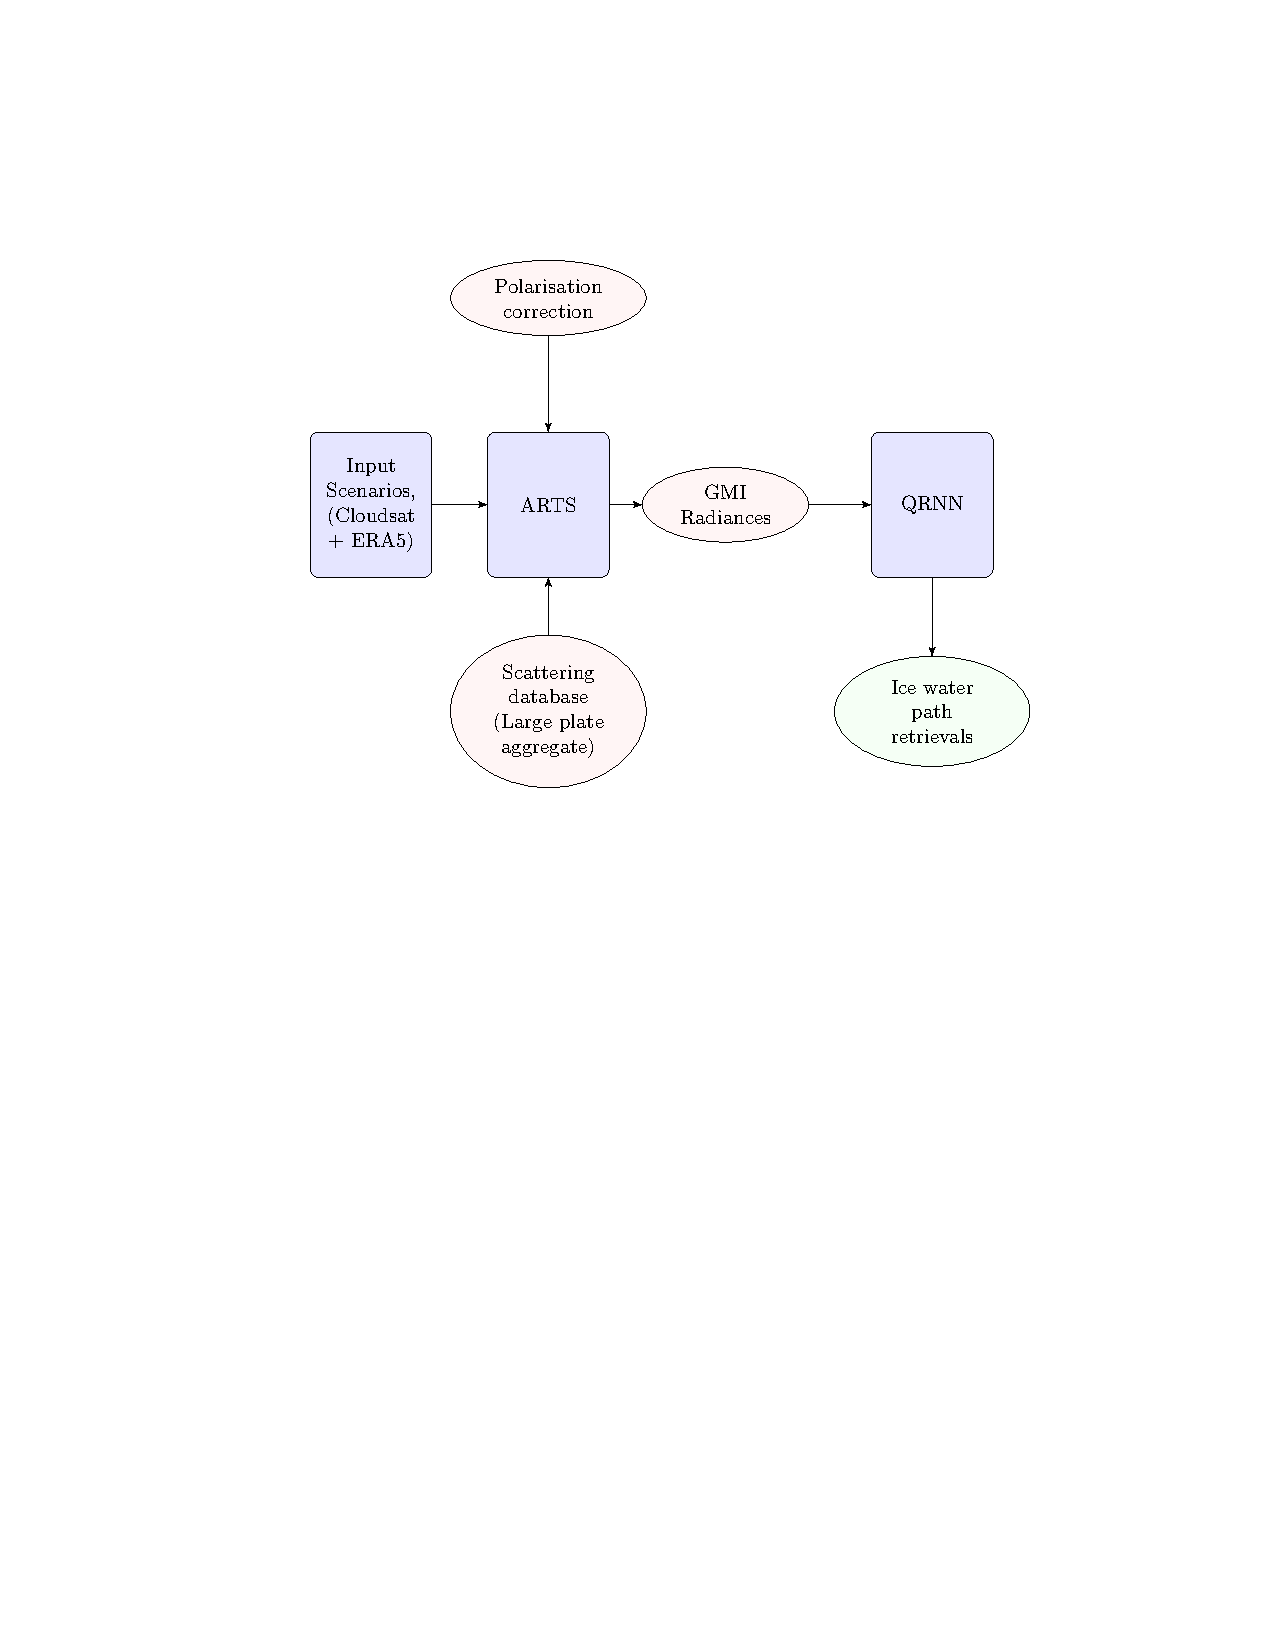
\includegraphics[trim=100 410 100 125,clip,height = 50mm, ]{Figures/flowchart.pdf}
	\caption{Flowchart showing the retrieval system.}
	\label{fig:flowchart}
\end{figure}

The main idea of this study is to generate a database of GMI measurements based on radiative transfer which includes oriented particles, and then combine it with machine learning (ML) to retrieve IWP. In this way, the impact of orientation on retrieval accuracy can be quantified. Figure~\ref{fig:flowchart} provides a flowchart of the scheme. The ML algorithm (Sect.~\ref{sec:QRNN}) uses the database to give the posterior knowledge of the quantity sought, given the scene of observations. Using ML on a retrieval database for inverting TB to IWP has advantages over the traditional inversion techniques because ML can avoid the uncertainties introduced by approximations. 

\subsubsection{QRNN}
\label{sec:QRNN}

The retrievals are based on a neural network based method called Quantile Regression Neural Network \citep[QRNN,][]{pfreundschuh:aneur:18}. QRNN is a neural network which learns to predict a vector of quantiles {$y_i$} representing the distribution of the output from a set of inputs {$x_i$}, through a series of learnable transformations. While training, the network seeks to minimise the model error through a quantile loss function. If $x_{\tau}$ is the $\tau$th quantile of a cumulative distribution function $F(X)$, the quantile loss function is defined as:

\begin{equation}
\mathcal{L}_\tau(y_\tau, y_{true}) = \begin{cases}
(1 - \tau)|y_\tau - y_{true}| & \text{if}  y_\tau < y_\text{true}\\
\tau |y_\tau - y_\text{true}| & \text{ otherwise, }
\end{cases}
\label{loss_function}
\end{equation}

QRNN is available open source software quantnn \citep{} implemented with PyTorch backend \citep{paszke2017automatic}. The optimal QRNN configuration implemented for this study is described in Appendix~\ref{app:qrnn_conf}

The output of QRNN is the posterior distribution of the estimate. This is different from the conventional retrieval methods which provide single point estimates. The quantiles quantify the prediction uncertainty through a probabilistic upper and lower bound for each case. While the posterior distribution has it own advantages, but for evaluating retrieval accuracy, usually the median quantile or the  expectation value $\mathbb{E}[y]$ as the point estimate is chosen as the point estimate. In this study, the point comparisons are made with the $\mathbb{E}[y]$. 
 
%\subsection{QRNN trainings}
%\label{sec:qrnn_trainings}
%To scrutinize the impact of databases on the retrieval performance, a separate QRNN is trained for each of the two databases : LPA-ARO, LPA-TRO(sect.~\ref{sec:database}). The basic construction of all trainings is identical (sect.~\ref{sec:QRNN}), except for the input database each is based on. 

%Furthermore, two additional QRNN trainings are considered to monitor the impact of oriented hydrometeors. These two trainings are based on databases LPA-ARO and LPA-TRO, but the input data is slightly different. Here, instead of including both polarisation channels of 166\,\,GHz, only the V-polarised channel is included.

%For each training, around 950\,000  simulations are used for training and around 200\,000 simulations are used for validation during the training. The validation data is the part of the dataset which is used during the development of the training algorithm to quantify its performance. This dataset is different from the test data, on which the results are based on. Additionally, another set of LPA-ARO simulations consisting of 100\,000 cases is used as a test dataset to evaluate the  basic retrieval performance. These simulations are not revealed to QRNN during training. 

%\subsection{Evaluation metrics}
%\label{sec:evaluation}

%In this study, a statistical comparison of the simulations and observations is made. If $P^o$ and $P$ are two probability distributions and $KL (P^o \parallel P)$ denotes the Kullback–Leibler divergence between the two, then square root of the J-S divergence is defined as:
 
%\begin{equation}
%JSD(P^o \parallel P) = 0.5 \times (D(P^o \parallel R)+D(P \parallel R))
%\end{equation}

%where, $R = 0.5 \times (P^o + P)$ is the mid-point of the probability vectors $P^o$ and $P$. $JSD$ can take values between $[0, \inf]$, where small values indicate low divergence. $JSD$ is equal to zero only if $P^o$ and $P$ are identical distributions. For two-dimensional distributions, the divergence can be calculated along both dimensions.

%Further, to evaluate the accuracy of the retrievals, it is crucial to describe on the output of QRNN. 

 %We select commonly used metrics such as bias and mean absolute error (MAE). An additional metric known as fractional error (FE) is also used. Due to the dynamic range of IWP, FE has been utilised by \citet{holl:spare:14, brath:micro:20}  to compare the accuracy of retrieved IWPs. If $y_o$ and $y_r$ are the reference and the retrieved IWPs, respectively, the FE is defined as:

%\begin{equation}
%FE = e^{\log\left|\frac{y_r}{y_o}\right|} - 1
%\end{equation}

\section{Results}

\subsection{Polarisation ratio}
\label{sec:polratio_selection}

The polarisation effects introduced by oriented particles and observed by conically scanning instruments \citep{gong:micro:17} were replicated by \citet{barlakas:intro:21}. They introduced a a simple scaling factor which mimics the differences between H and V polarisations caused by ice hydrometeor scattering. For TRO particles, the scattering is isotropic, hence there is no difference in the extinction of between the two polarisations. However, oriented hydrometeors due to dichroism effects, introduce differences between the two, and the correction factor is a simple way to approximate this effect. To model the effect of ARO particles, a correction factor ($\alpha$) is used to increase and decrease the layer optical thickness ($\tau$) in the H- and V-
polarised channels, respectively, and the ratio of the modified layer optical thickness gives the polarisation ratio:

\begin{eqnarray}
\rho = \frac{\tau_H}{\tau_V} = \frac{1+\alpha}{1-\alpha}
\end{eqnarray}

The factor $\alpha$ $(>= 0)$  weakens the extinction at V-polarisation and strengthens it for H-polarisation. The polarisation effects can be described by shape and orientation of the hydrometeor, and the factor $\alpha$ can be indirectly understood as the axial ratio of an oriented hydrometeor. For TRO hydrometeors or circular polarisation, $\alpha$ is equal to one, and for ARO, $/alpha > 1$. 

\citep{barlakas:intro:21} found the best estimate of $\rho$ by comparing the polarisation signals between observations and simulations. \citet{gong:micro:17} have shown that variation of PD with TB follows an arch or bell shape pattern, which appears universally at all high microwave frequencies.  They suggested $\rho = 1.4$ ($\alpha$=1.67, for 166\,\,GHz). However, this value of $\rho$ cannot be used directly in our study for various reasons. Firstly, the passive monitoring experiments conducted to simulate GMI radiances are at model resolution. The GMI observations are ``superobbed'' on 80 $\times$ 80 grid meet the model resolution. Lowering the resolution limits smears out the maximum and minimum observed PDs. At the model resolution, the maximum PDs observed by \citet{barlakas:intro:21} lie around 20\,K but \citet{gong:micro:17} show that PDs as high as 30\,K occur frequently over water. Furthermore, in the latter, low PDs (< 5\,K) occur for the entire range of TBs, but the former such signals only exist for TBs > 200\,K. Due to differences in PDs at footprint and model resolution the effective value of $\rho$ could potentially be different. Another reason for missing low PDs could be shortcoming of RTTOV in correctly simulating the deep convection systems. RTTOV simulates warmer TBs for deep convection systems. Such systems are often associated with low PDs due to high turbulence, thus the full arch spread of PDs cannot be simulated. In RTTOV framework, the best performing $\rho$ was selected on the basis of only high PDs. The lower values of $\rho$, which deemed inappropriate in RTTOV framework could very well be important for the part of missing arch shape. Further for numerical weather prediction (NWP) the simulations are conducted to match the observations in space and time. But in this study, we are looking for a statistical consistency between both over a period of one month, which implies that the simulation dataset should demonstrate a larger variability.  Intuitively, the value should still be close to as suggested by \citet{barlakas:intro:21}, but requires comparison of the distributions of the forward modelled radiances and observations. However, the last argument could  indicate that some perturbation in $\rho$ could be necessary.
Besides the scheme described herein, another attempt at parametrising the polarisation signals observed from GMI at 89 and 166\,GHz has been made by \citet{galligani:param:21} with some promising results. However, the biggest limitation of their method is the need of dual-polarisation observations to derive the parametrisation. For instance the polarisation signals at 183\,GHz cannot be parametrised due to lack of H-polarisation, but that does not imply that effects of orientation can be ignored. Similarly an extension to sub-mm wavelengths shall be incomplete with the limited observations available.  

Multiple experiments with different values of $\rho$ were conducted. All these experiments have similar set up of microphysical assumptions for consistency. In first five experiments, forward modelled radiances are estimated for $\rho = 1,1.1, 1.2, 1.3, 1.4$. Two more experiments, but with values of $\rho$ belonging to a distribution are also performed. In these two experiments, the choice of $\rho$ is motivated by the results with constant $\rho$, and are described in detail in the next section.  In this section, we utilize the PD-TB$_V$ relationship at 166\,\,GHz to select the value of $\rho$ providing the best fit between simulations and observations. Polarisation signals can also originate from surface contaminations, and they have been filtered out for this comparison.  The  ``3$\sigma$'' method described by \citet{gong:micro:17} has been used to filter out the clear-sky cases. This method uses the TBs at 183$\pm$3\,GHz to define a threshold (T$_o$), and if  $\sigma$ is the standard deviation of the probability density function of the TBs, then all cases with TBs < T$_o$ - 3$\sigma$ are classified as cloudy. Stringent filtering can remove surface contamination, but at some cirrus signatures can also be removed. 


% (Sect.~\ref{sec:polratio}). Two distribution of $\rho$ are defined. First is a truncated normal distribution with mean = 1.2, and standard deviation 0.12, and second is a uniform distribution for $\rho\in[1, 1.4]$. There were good reasons to not to inspect values higher than 1.4 in these distributions. We describe them  in Sect.~\ref{sec:polratio}. 



\subsubsection{Selecting optimal polarisation ratio}
%
\begin{figure*}[t]
	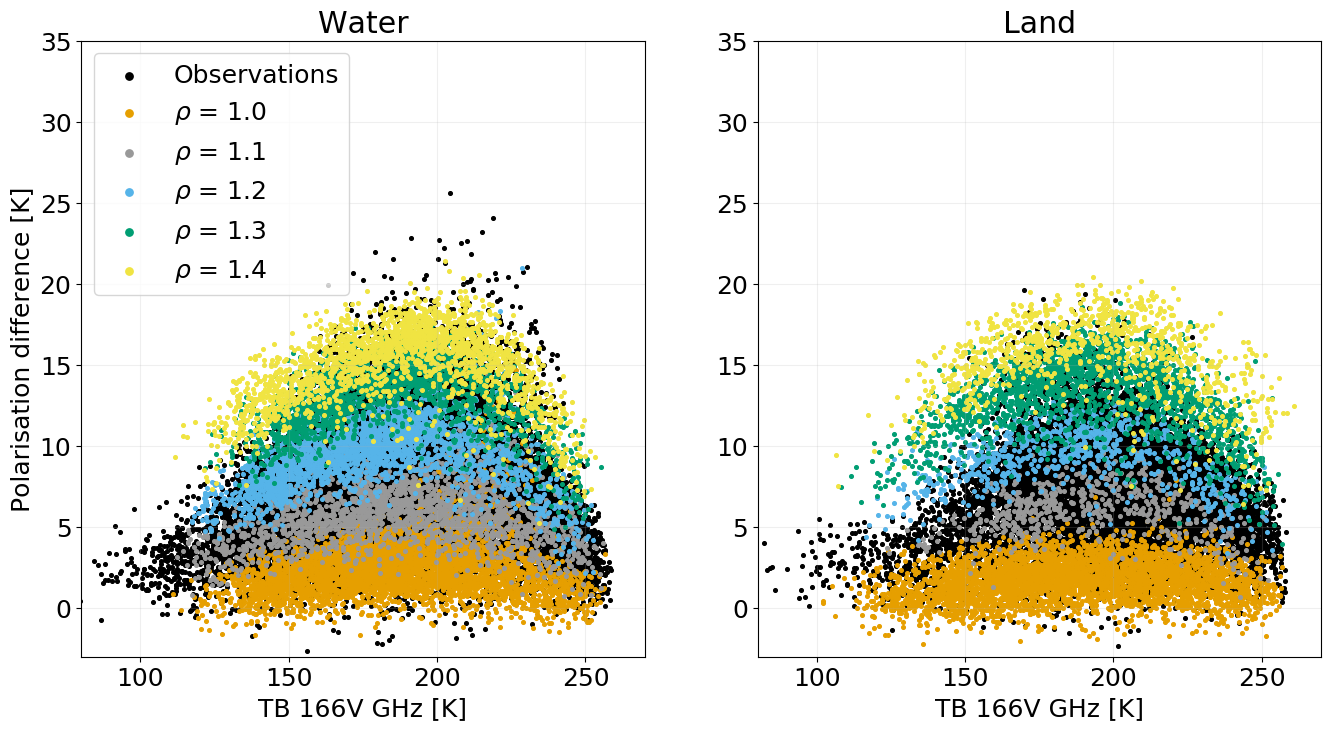
\includegraphics[width=10cm]{Figures/PD_water_varying_rho_water_land.png}
	\caption{The polarisation differences (166V - 166H) as a function of brightness temperatures at 166V GHz ( PD-TB$_V$ relationship) for observations shown in black. The simulated PDs are for different values of $\rho$ are denoted by different colors. }
	\label{fig:PD_166}
\end{figure*}
\begin{figure*}[t]
	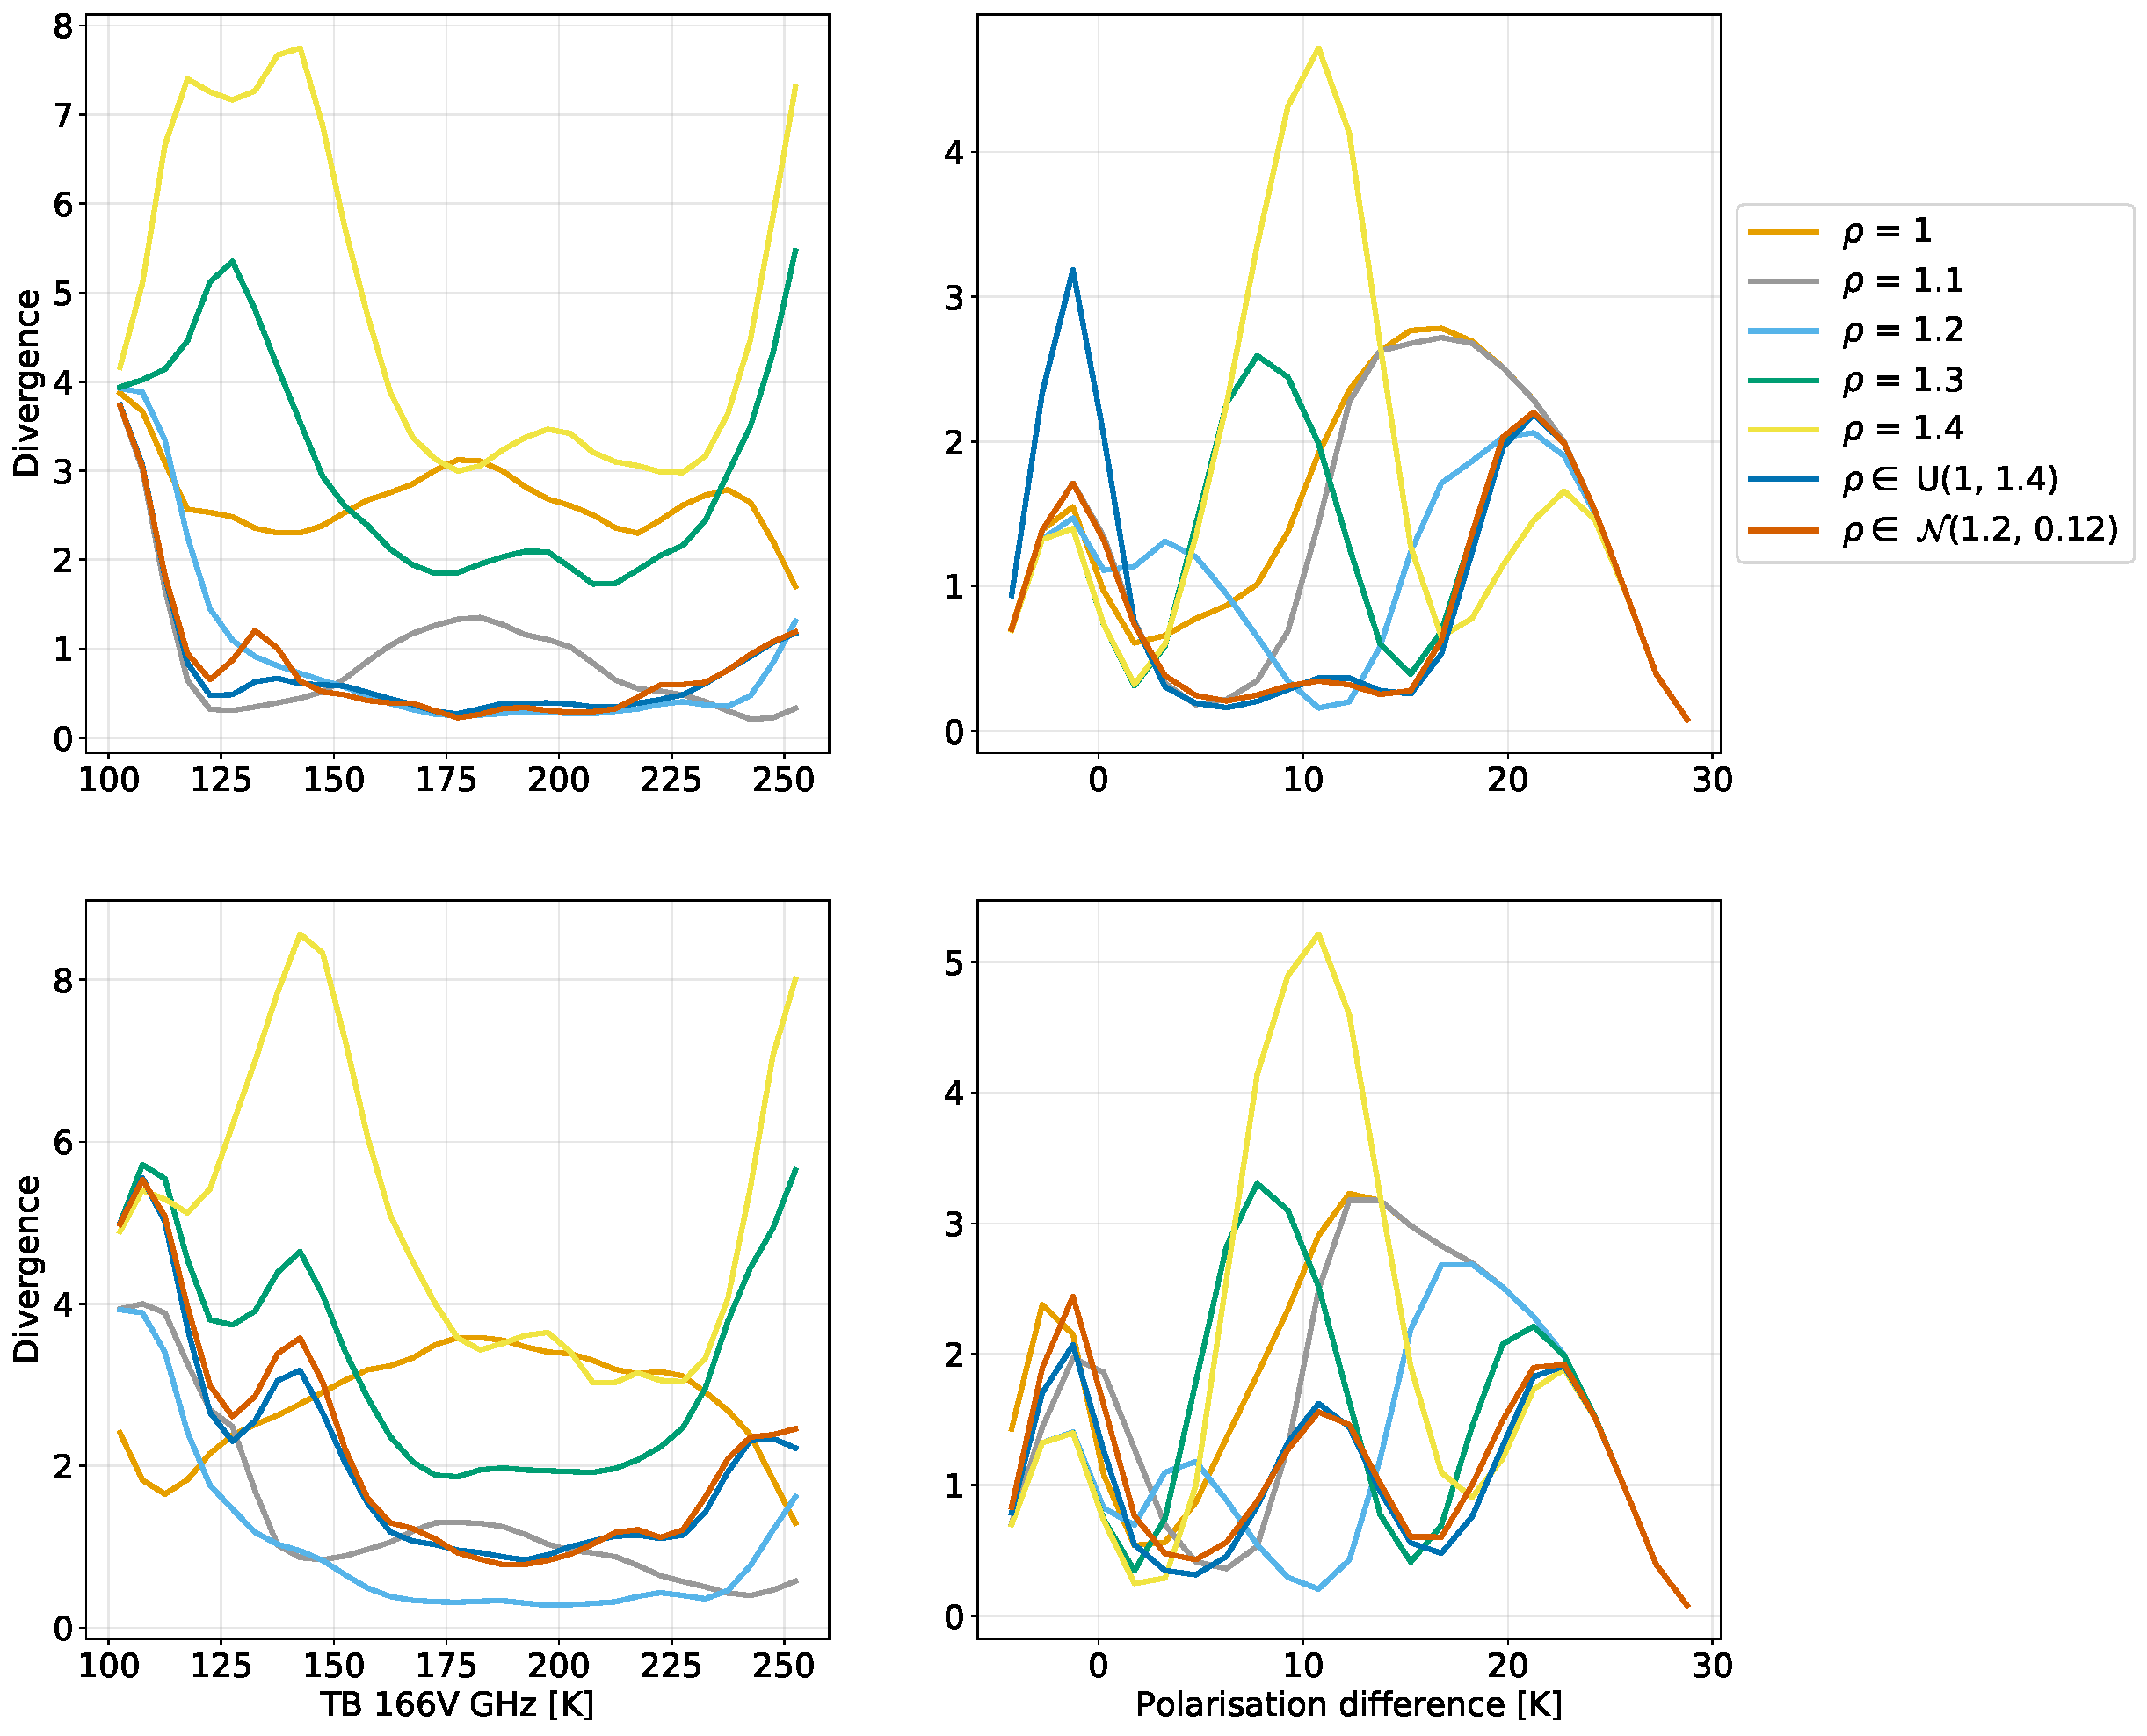
\includegraphics[width=10cm]{Figures/divergence_land_water.pdf}
	\caption{The KL divergence describing the differences between the two-dimensional PD-TB$_V$ relationship between observations and simulations along (a) TB axis and (b) PD axis over water. Results from the five experiments with different values of $\rho$, uniform distribution (U(1.0, 1.4)) and truncated normal distribution ($\mathcal{N(1.2, 0.12)}$) are shown. }
	\label{fig:divergence_PD_land_water}
\end{figure*}



%\begin{figure}[t]
%	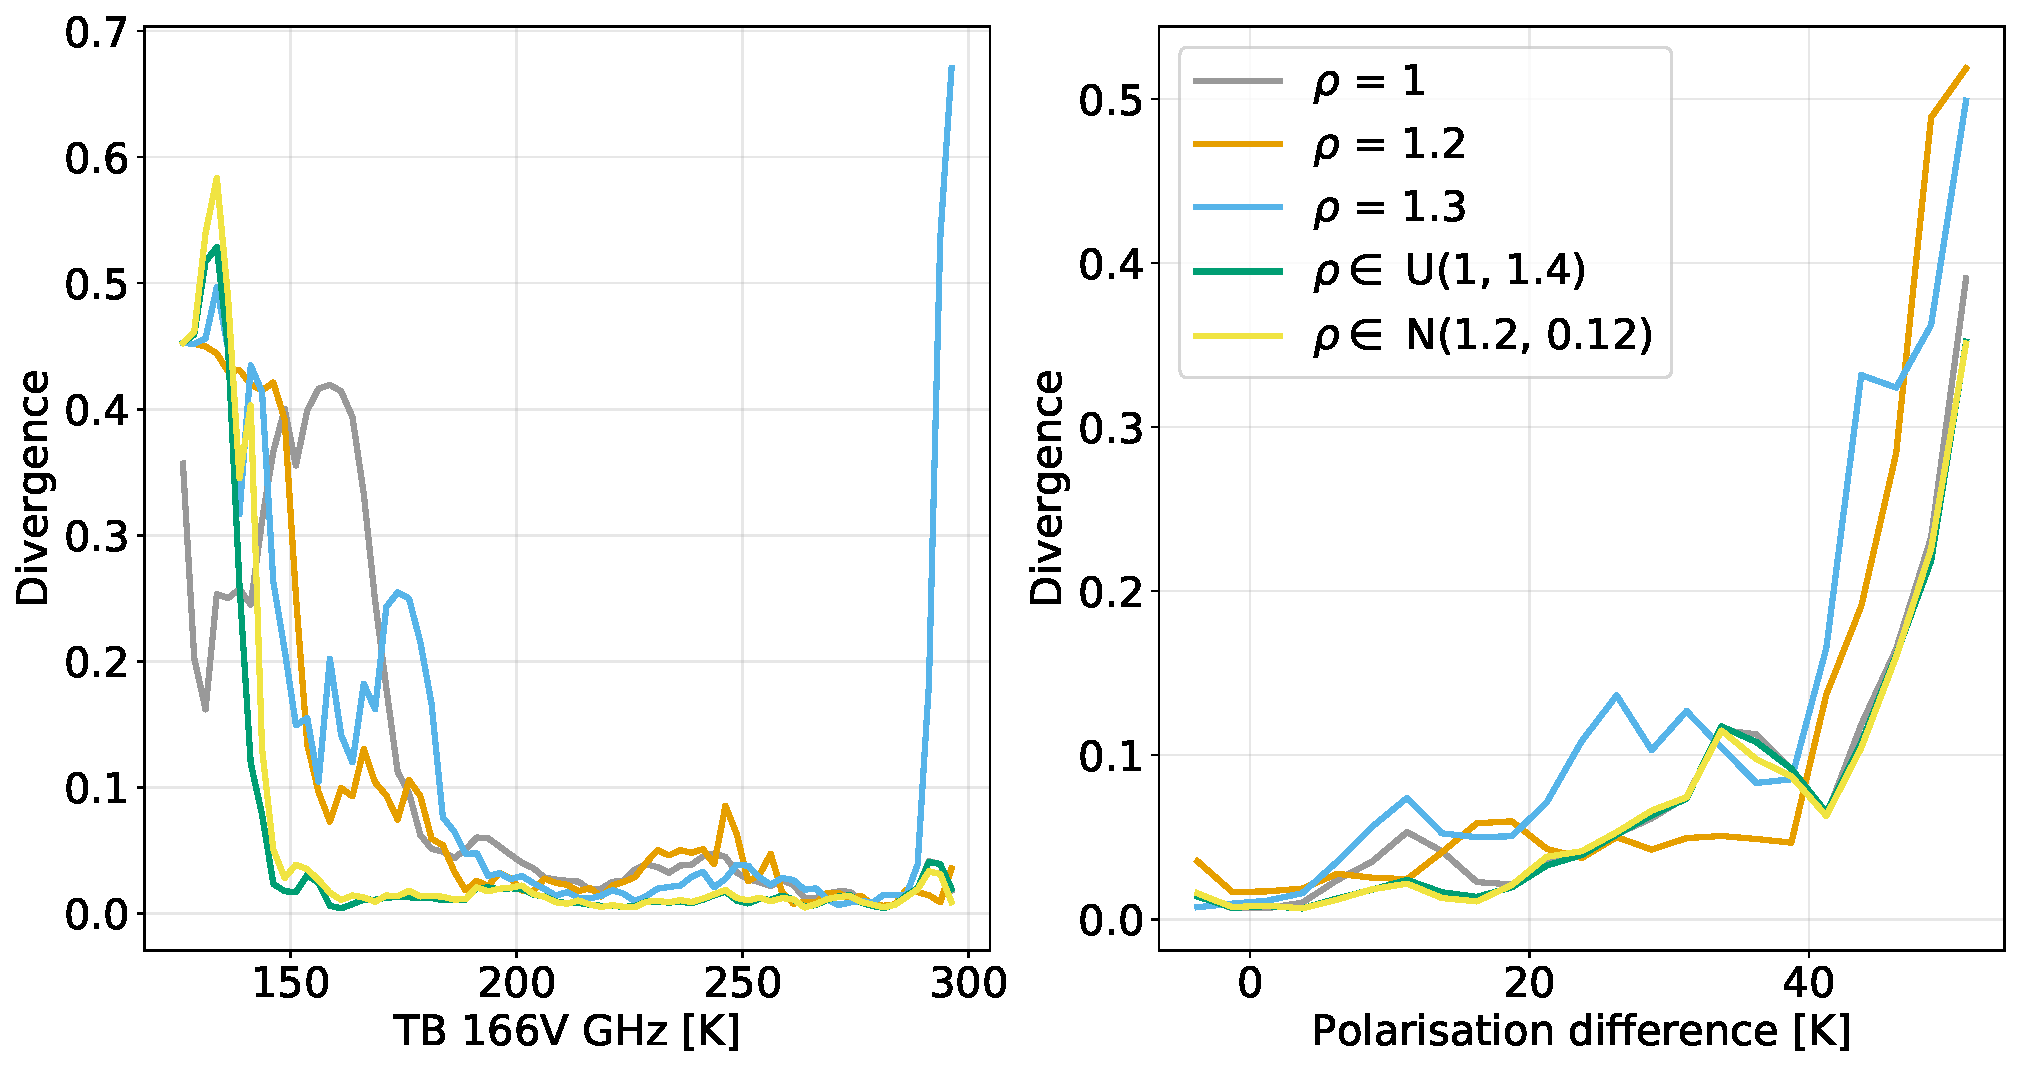
\includegraphics[width=8.3cm]{Figures/divergence_esa.pdf}
%	\caption{ Same as Fig.~\ref{fig:divergence_PD}, but with evans snow aggregate.}
%	\label{fig:divergence_esa}
%\end{figure}

Figure~\ref{fig:PD_166} shows the PD-TB$_V$ relationship obtained while using a constant value of $\rho$ over water and land. Here the simulations do not have a one-to-one correspondence with the observations. But it is also not necessary to evaluate the performance of $\rho$. We are only interested in the match between the two distributions in a statistical sense. In fact, the four datasets shown in the figure do not come from identical synthetic scenes, but have almost identical number of cases (\todo{give number}) and are from the same month, January. Some statistical fluctuations due to inconsistency between the datasets can be expected, but it should not alter the overall behaviour significantly. Furthermore, Fig.~\ref{fig:PD_166} only provides a qualitative view, so in order to quantify the measure of similarity between the observed and simulated PD-TB$_V$ distributions, we employ the Kullback–Leibler (KL) divergence \citep{Joyce:kl:11} to calculate the fit between two-dimensional histograms of observations and simulations. While estimating the histograms some bins end up as empty. Such bins are replaced by a small number to avoid infinite penalty. The divergence results over water and land are displayed in Fig.~\ref{fig:divergence_PD_land_water}.

We will firstly discuss results over water. When $\rho = 1$, no orientation effects are simulated and the maximum PD is observed to be around 5\,K, but most cases are close to zero PD. While this is also an important part of the observed distribution, the high PDs are completely missed and this is also indicated by high divergence along both TB and PD dimensions. As $\rho$ increases, the impact of the orientation comes into play, and the distribution of PDs moves towards higher values, and this is also reflected as a dip in divergence along the PD dimension.  $\rho = 1.4$, can simulate most of the highest observed PDs between 15 and 20\,K, but some extremely high polarisation signals are missed. While $\rho$ > 1.4  could be included to reproduce the few cases with extremely high PDs (> 20\,K) but it shall also increase the PDs over the slopes on either side of the peak. Already some impact of over-representation is reflected for $\rho =$ 1.3 and 1.4 in region with TBs > 225\,K and TBs < 150\,K. While some extra variability in the simulations, but within physical limits is acceptable, $\rho > 1.4$ seems unfeasible at least in the current set of microphysical assumptions. \citet{barlakas:intro:21} also showed that values greater than 1.4 lead to an increasing mismatch between the observations and simulations. Further, among all simulation datasets shown here, none is able to reach the lowest end of the TBs, and this is reflected by the high divergences below 125\,K. From the scatterplots it is obvious that constant value of $rho$ cannot reproduce the entire range of observed PDs, but it is  interesting to see that lowest differences occur for  $\rho = 1.2$. This suggests that 1.2 is an important value which can reproduce the polarisation signals following the median of PD-TB$_{v}$ relationship. This maximum of the PD median is reflected by the drop in divergence along the PD dimension. The maximum PD for $\rho = 1.2$ is 12\,K. This is comparable to the PD median calculated by \citet{galligani:param:21}. 

Over land, quite similar effects are seen. Although, the magnitude of maximum observed PDs is slighly smaller than over water. Additionally, the spread of polarisation signals is narrower. Despite that $\rho = 1.2$ again represents the median of PD-TB$_{V}$ relationship. Due to lower spread of PDs $\rho$ between 1.3 and 1.4 also introduces some over-representation of PDs over the slopes of the arch. 

Nevertheless, for both water and land, each value of $\rho$ fails at reproducing the entire distribution of PDs and can replicate only a part of the observed distribution. This suggests that a variation in $\rho$ is necessary to replicate the variety in polarisation signals. Based on the above results, we propose two different distributions for $\rho$: a uniform distribution between 1 and 1.4, and a truncated normal distribution between 1 and 1.4. Both distributions are centred around 1.2. While a slightly smaller upper limit could be feasible for land, we choose identical $\rho$ distribution over both land and water. The slight relaxation is allowed over land mostly because of two reasons. Firstly, polarisation ratio independent of surface type is straightforward to implement, but the additional advantage is to account for variability of surface types not included in the comparison. We do not consider ice scattering signatures over coastlines, snow, seaice and other mixed surface types in deriving the optimal value of $\rho$. 

A comparison of the uniformly and truncated normally distributed $\rho$ is also depicted in Fig.~\ref{fig:divergence_PD_land_water} by dark blue and red color respectively. Over water, with both distributions of $\rho$, the match between the observations and simulations is quite high. Maximum differences are observed for coldest TBs which as seen earlier cannot be simulated within our current radiative transfer set-up. Along the PD dimension, combine effect is visible 

Over land, however a slightly different behaviour is observed. With both distributions of $\rho$, the overall match between the observations and simulations increases, but is not the best. Due to a narrower bell curve over land, simulating the highest observed PDs, comes at the cost of some extra polarisation signals between 10 and 15\,K. These deteriorates the overall match between the observed and simulated. The effect of extra polarisation signals is also reflected in the high divergence. Since here we are not looking at one-to-one correspondence between the simulations and observations, a slightly larger variability in the simulations but within the physical limits of measurement space should be acceptable.

Finally, among the two distributions of $\rho$, the uniform distribution emerges to be better performing but only with small margin. It is has slightly better results towards the TB depressions and higher PDs. Thus a distribution centered around 1.2 is a requisite, but cases with random orientation and extremely PDs should also be equally represented. A truncated normal distribution with larger variance should also give comparable results. 

Additionally, we also explored the effective range of $\rho$ for evans snow aggregate. These results are described in Appendix~\ref{app:esa}. 


\subsubsection{PDs over land and water}
%
\todo{how this sect should be presented?}
\label{sec:PD}
\begin{figure}[t]
	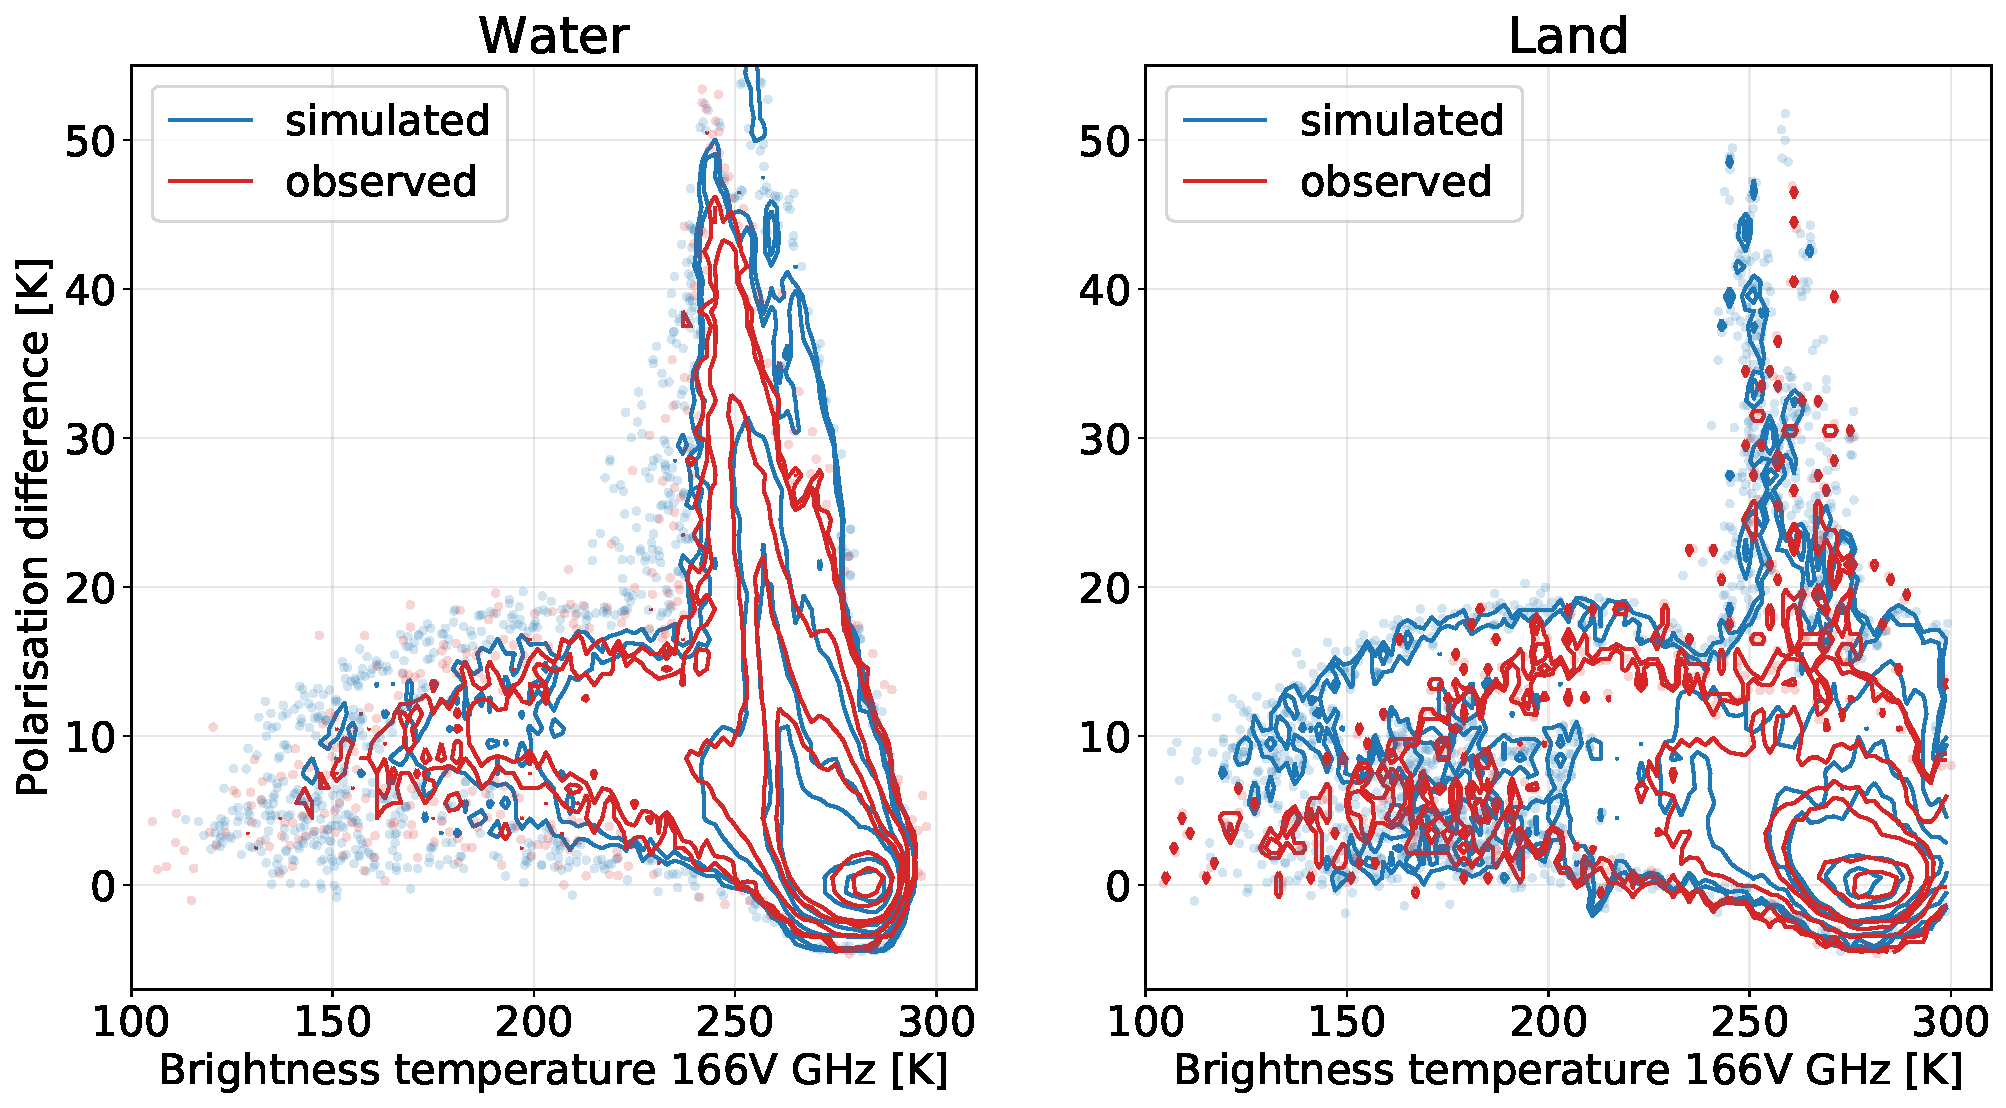
\includegraphics[width=6cm]{Figures/hist2d_land_water_jan.pdf}
	\caption{Polarisation differences (166V - 166H) as a function of
		TB 166V GHz for observed (red) and simulated (blue) for
		different surface types. The curves denote the maximum probability of the two-dimensional histogram. The low density points are plotted as dots. }
	\label{fig:PD_water_land}
\end{figure}

Figure~\ref{fig:PD_water_land} shows the observed and simulated PDs. PDs from surface contribution are not filtered out. For both surface types, the TB-PD relationship is characterised by a strong arm consisting of very high PDs centered around 250\,\,K and a cluster of cases forming a arch like structure. The strong vertical arm is due to polarisation signals introduced by surface emissions. The strongest PD are observed over land and water under dry atmospheric conditions. In the presence of water vapour, the signal from the surface is attenuated and the PDs cluster around the bottom tip of the distribution. 

As earlier mentioned, we are highly interested in the arch region, where maximum impact of ice hydrometeors lies. For land and water the arch is quite strong. For these surface types, the maximum PD (~20\,\,K) are centered around 200\,\,K. The PDs diminish towards the colder TBs, while towards the warmer end, the PDs from clear-sky overlap. \citet{gong:micro:17, galligani:param:21} describe these PDs in detail. The overall arch shape arises from the combined effect of ARO and TRO particles. The horizontally aligned particles produce the maximum PD and these particles are usually part of convective outflow regions like anvil. However, in turbulent systems, the multiple scattering processes decrease the PDs. The lowest observed PDs are close to 0\,\,K, which occur for the coldest TBs, representing the deep convection systems. The negative PDs also occur, but they are mostly associated with the clear-sky measurements affected by noise. 

\subsubsection{PDs at 660\,GHz}
%
\label{sec:submm_pd}
\begin{figure}[t]
	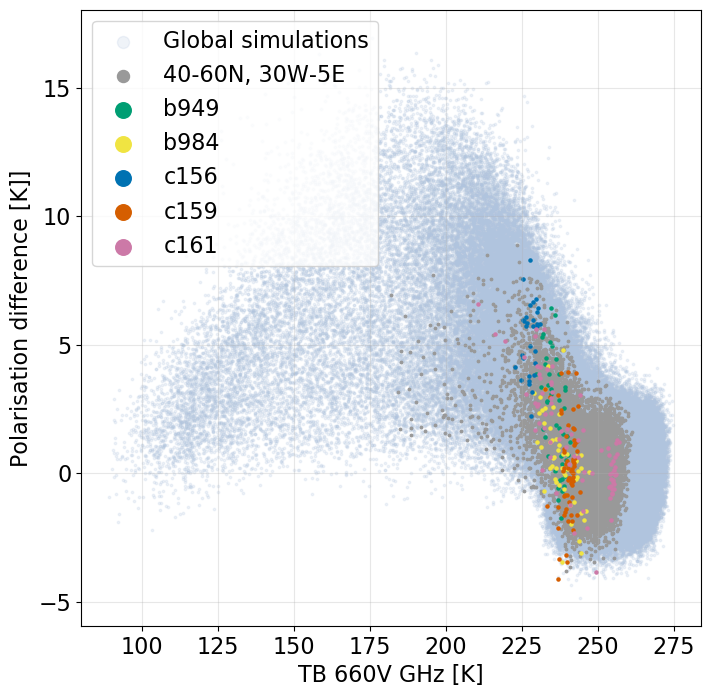
\includegraphics[width=4cm]{Figures/PD_660.png}
	\caption{The scatter plot showing the PD vs TB$_v$ at 660\,GHz. The light blue dots are for near global simulations; the gray dots denote simulations in 40$^{\circ}$N - 60$^{\circ}$N/30$^{\circ}$W-5$^{\circ}$E. The five alphanumeric codes depict observations from five flight campaigns as described by \citet{fox2020evaluation}}
	\label{fig:PD_660}
\end{figure}

With the increasing interest towards sub-mm frequencies, we also simulated the polarisation signals at 660\,GHz using $\rho\in U[1, 1.4]$ (Fig.~\ref{fig:PD_660}). In this plot, filtering of cases with surface contamination is not considered. The arch shape of PDs is preserved at 660\,GHz and the maximum PD is around 15\,K which occurs for TB around 190\,K. 660\,GHz is not sensitive to surface (weighting function peaks in the upper troposphere), hence the high PDs associated with surface contamination are missing. Similar results were obtained by \citet{gong:micro:17}, who analysed Compact Scanning Submillimter-wave Imaging radiometer (CoSSIR) 640\,GHz measurements. These observations were mostly over the Pacific Ocean near Central America, and the maximum amplitude of PDs was observed to be 10\,K.

We also compared our simulations with observations from five flight campaigns by the Facility for Airborne Atmospheric Measurements (FAAM) BAe-146 research aircraft. These flights flew around UK during March 2016, 2019 and October 2016. More details about these flights is described in Table 2 of \citet{fox2020evaluation}. The observations are averaged at 6\,km along track to match the GMI resolution. Out of the five flights shown, C161 has the highest observed IWPs that correspond to PDs greater than 5\,K. A part of this flight had clear-sky conditions which is reflected by the cluster of observations around 260\,K. Most of the observations made by flight C159 are in clear sky conditions \citep{fox2020evaluation} and they have negative PDs which are most likely due to noise. Such values are also observed by B994 during the initial and final leg of the flight. 


\subsection{Snow emissivity model}
\label{sec:snow_emissivity}

For water bodies the TESSEM model is valid to sufficiently high frequencies, but for other surface types no ready models are at hand and estimates of land, ice and snow emissivity. The climatology based TELSEM has an updated version TELSEM2 \citep{wang:surfa:17}, which provides an emissivity database for land, sea ice and snow surface types above 85 GHz. However, in the latter,  the snow and sea ice emissivity estimates are empirical approximations. For example, continental snow emissivity values are assumed to be constant for frequencies above 85 GHz. The sea ice emissivities are parameterized upto 183 GHz using Special Sensor Microwave - Imager/Sounder (SSMIS) derived emissivities \citep{boukabara2011mirs} but only for recent sea ice classes. Multi year ice emissivities are assumed constant for frequencies above 85 GHz. On the other hand, data from aircraft campaigns (e.g. \citet{hewison:2002:airbo}) have shown that emissivity at 183 GHz is consistently higher than at 157 GHz for both snow and sea ice surface types. Similarly, \citet{harlow:2012:tundr} have also shown that the snow emissivities increase monotonically with increasing frequency. 

Based on the observations in these studies, we have developed an empirical snow emissivity model for frequencies between 150\,\,GHz and 190\,\,GHz. This model gives a random estimate of the snow emissivity from a standard normal distribution depicting the valid range of emissivity values. It is not important to know the exact snow emissivity at a given time and position, but the distributions of simulated emissivities should follow the reality. The basic idea is to find a set of emissivity estimates that simultaneously give radiance closest to the measurements. This empirical model was fine-tuned by comparing the observed and forward modelled TBs, and the final version used in this study is described below. 

If $\epsilon_{193}, \epsilon_{159}$ represents the emissivities for 193\,GHz and
159\,GHz respectively, then
\begin{align}
\epsilon_{193}& = \min({N(\mu_{193}, \sigma_{193}^{2}), 1});\, \mu_{193} = 0.78, \sigma_{193} = 0.07 \label{eq:1}\\
\epsilon_{159}& = \min(\epsilon_{193} - N(\mu_{159}, \sigma_{159}^{2}), 1) ;\,  \mu_{159} = 0.02, \sigma_{159} = 0.02\,\label{eq:2}
\end{align}
where, $N(\mu, \sigma^{2})$ represents the standard normal distribution with
mean $\mu$ and standard deviation $\sigma$. The differences between the
H- and V- polarisations for both frequencies are 
approximated through a uniform random distribution.

\begin{align}
d_{159}& = U(a_1, b_1) ;\, a_1 = 0.005, b_1 = 0.055\\
d_{193}& = d_{159} - U(a_2, b_2) ;\, a_2 = 0.015, b_2 = 0.025 \,
\end{align}
where, $U(a, b)$ represents a uniform distribution between a and b. 

In this study, snow over both land and seaice were treated identically.
 
The range of emissivity estimates obtained from our model are also comparable to emissivity estimates from passive microwave instruments. For instance, \citet{munchak2020active} retrieve emissivities for GMI using optimal estimation method. They define 20 snow covered surface classes for which the emissivity estimates vary between 0.75 to 0.92. With randomness in our model, we also end up with similar emissivity estimates. Similar values were also reported by \citet{camplani2021passive} for snow covered surfaces.
 

\subsubsection{PDs over snow covered surfaces}
%
\begin{figure}[t]
	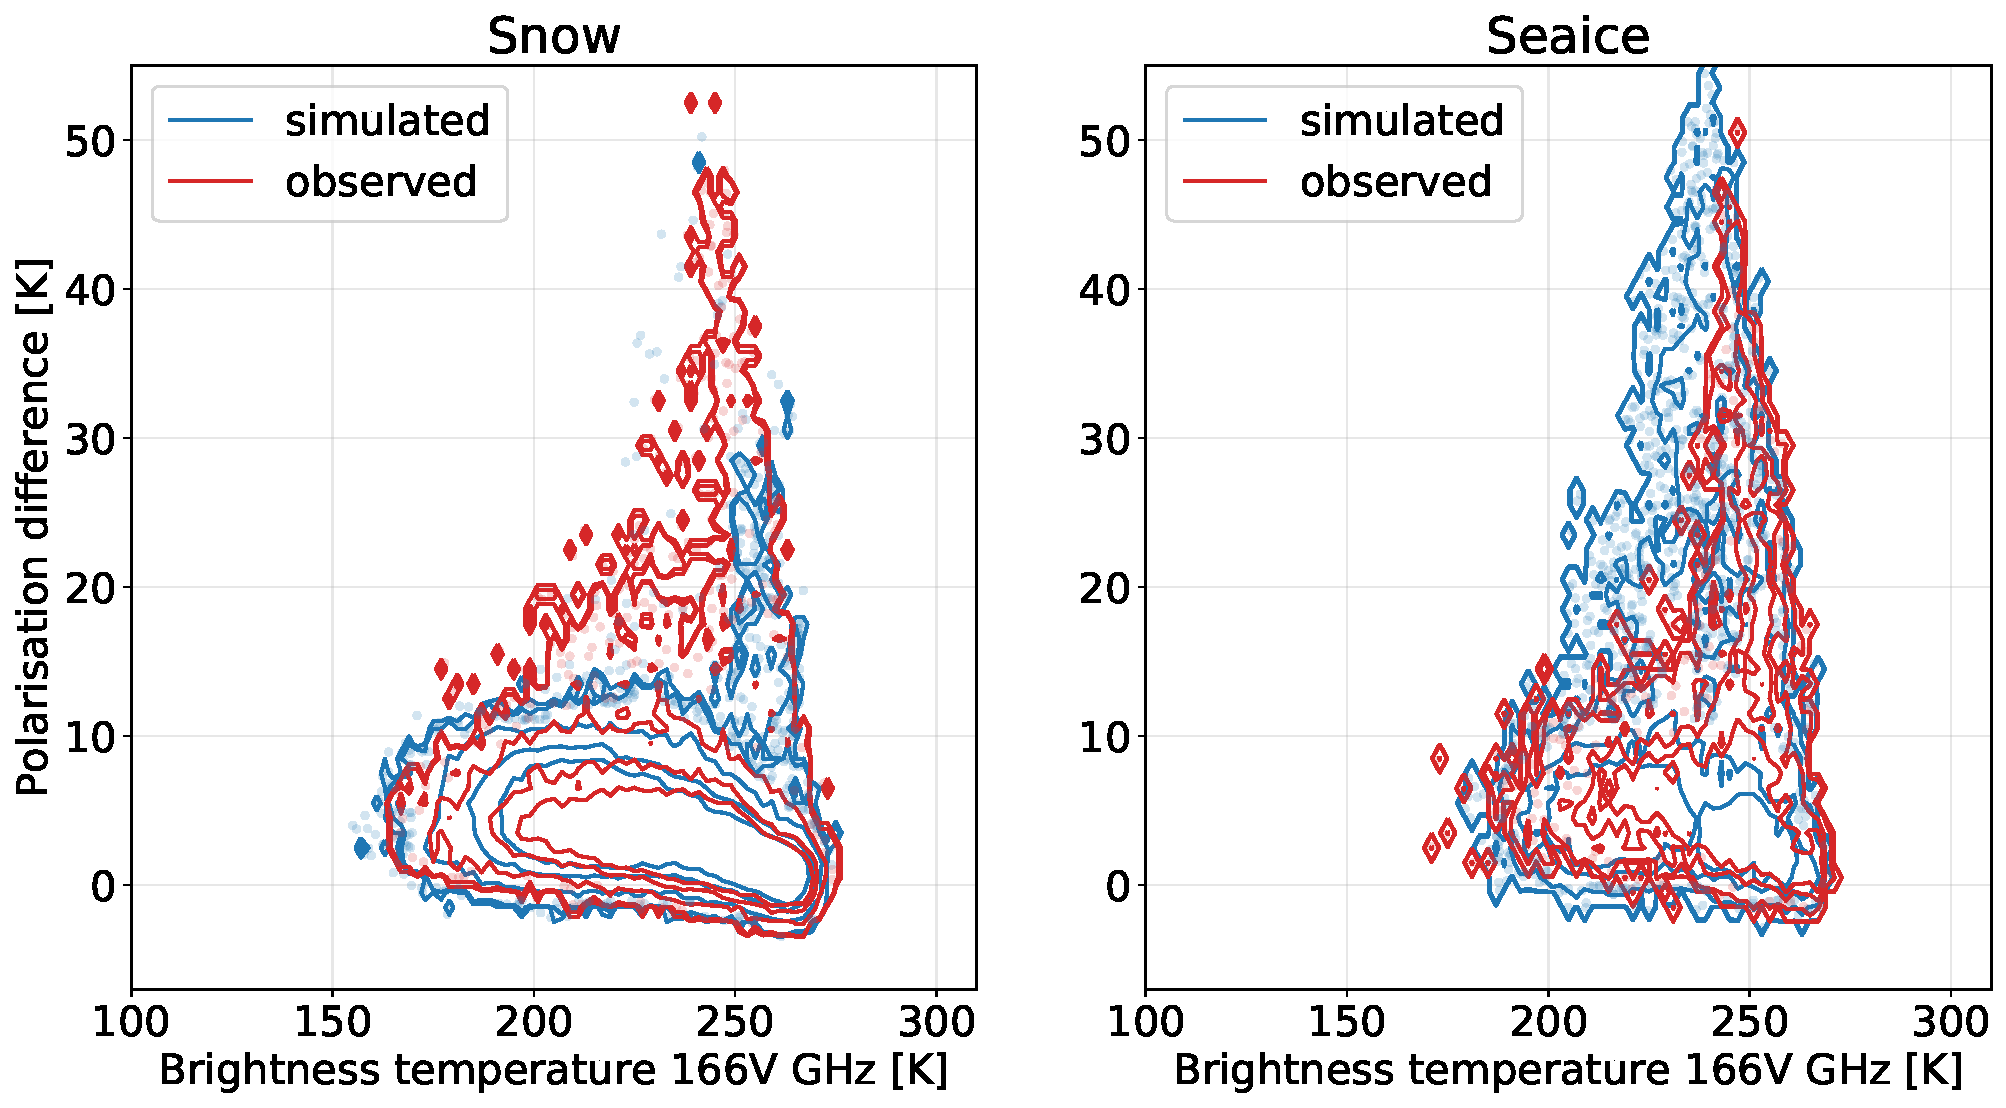
\includegraphics[width=6cm]{Figures/hist2d_snow_surface_jan.pdf}
	\caption{Same as Fig.~\ref{fig:PD_water_land} but for snow covered surfaces and seaice.}
	\label{fig:PD_snow}
\end{figure}

Figure~\ref{fig:PD_snow} shows a comparison of the observed and simulated PDs over snow and seaice surface types. All observations classified under seaice/water boundary and snow/land boundary are also included. It is clarified that for snow and seaice surface types, the distribution of PDs is combined effect of scattering signatures from surface and hydrometeor impact; no filtering is applied. However, the hydrometeor impact is expected to be small as high latitude winters scenarios are mostly associated with extremely dry atmosphere. 
  
For surfaces covered with snow, the PDs consist of a distinct arch type distribution with maximum PDs around 10\,K and an arm consisting of PDs as high as 50\,K. For the arch region, the match between observed and simulated PDs is quite high, which endorses that the snow emissivity estimated by the empirical model can replicate the real observation. On the other hand, the high PDs observed along the arm are suggestive of surface impact but from a non-snow covered surface or mixed surface type. An analysis of these cases along the arm revealed that they belong to snow covered surfaces lying close to water. GPROF classifies them under snow surface type, but they can potentially be classified under snow/water boundary. The pure snow surface induced polarisation signatures are clustered in the flat region. These can also overlap with PDs observed from ice hydrometeor scattering. Without any additional information, it would not be trivial to separate one type of signal from the other. 

Over seaice, the structure of PDs is slighly different than snow covered surfaces. Here the flat arch region is quite narrow and the concentration of observations along the arm is dense. It should be remember that in our emissivity model, seaice is assumed to be covered by snow, no other representation of seaice is considered. Snow over seaice only introduces PDs upto 10\,K as seen for pure snow covered surfaces over land. The higher PDs along the arm are a result of surface impact of mixed surface types such as seaice/water boundary. Interestingly, GMI observations belonging pure seaice surface class also have PDs along this arm. Since we do not consider pure seaice class in our database, it is difficult to attain a perfect match with the observations. For example, most of the cases along the arm lie close to land and could possibly be associated with thin seaice cover.  


\subsection{Comparison of simulations and measurements}
\label{sec:comparison_sim_obs}
\subsubsection{TB distribution and IWP}

\begin{figure}[t]
	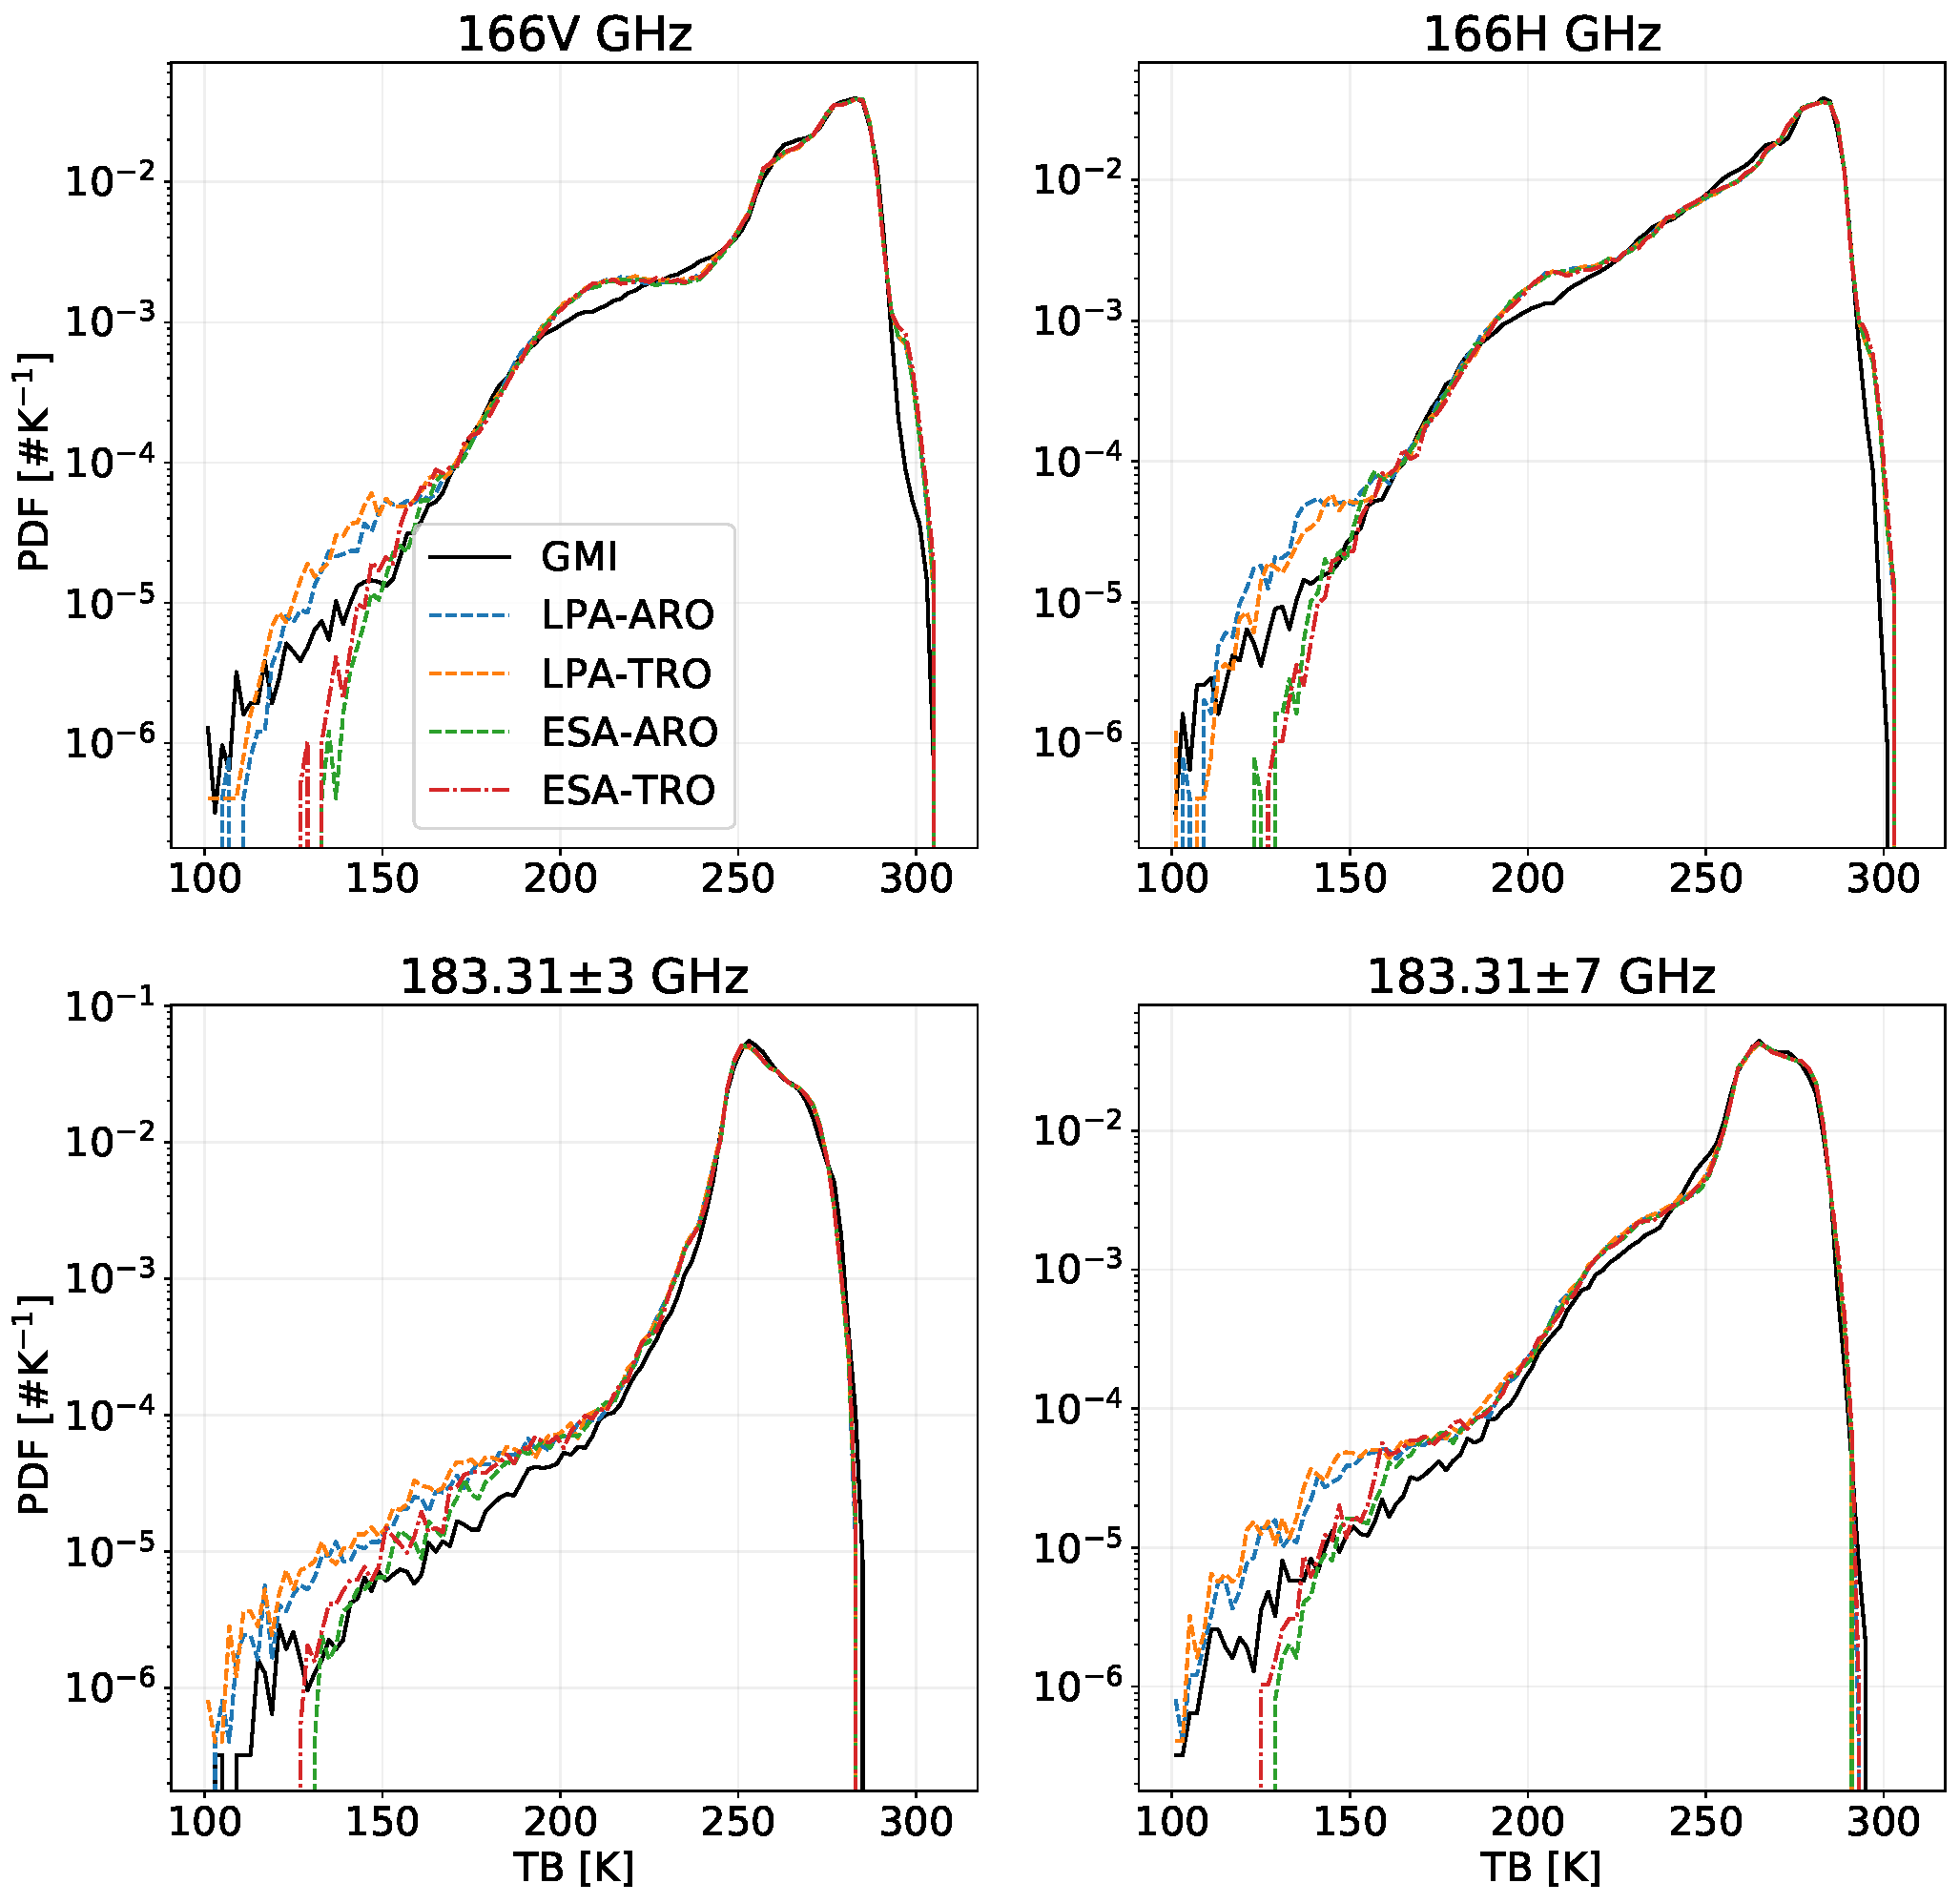
\includegraphics[width=8cm]{Figures/PDF_TB_jan.pdf}
	\caption{Distribution of TBs for all high frequency channels of GMI . The black curve represents the GMI measurements. The TB distributions from large plate aggregate.}
	\label{fig:hist_TB}
\end{figure}


This section describes the distributions of simulated TBs for all four high frequency channels of GMI. The simulated values are based on random Cloudsat profiles thus only a statistical comparison with the observations is made. It is not necessary for the simulations to be collocated with the GMI observations in space and time, but a similar variability between the two is expected. For retrieval to be successful, the database should reflect the realistic scenarios. 

Figure~\ref{fig:hist_TB} shows the distribution of simulated TBs for each channel and the two databases (sect.~\ref{sec:database}). The distribution of GMI observations is also plotted in black. For all four channels, the peak of the distributions correspond to the clear-sky scenarios, while the coldest TBs are associated with deep convective systems. For clear-sky cases, all four databases agree well with GMI.

However, over the colder part of the TBs none of the two databases is able to reproduce the exact distribution. With large plate aggregate, the forward simulations put more cases with low TBs. At the intermediate region (between 170\,\,K and 250\,\,K) the simulations have a high occurrence frequency for all channels except 183$\pm$3. Analysing the distributions according to surface type and latitudinal extent revealed that the mismatch is removed when TBs over snow surface type are not included (not shown). This could be due to the forward simulations having a larger representation of snow cases than GMI. Since snow cover is a variable quantity, a comparison between data from different time scales can introduce such artefacts. 

Inclusion of ARO particles has a small impact on occurrence frequency of colder TBs. When only TRO particles are simulated, the deep convection zone has a higher frequency of colder TBs for V-polarised channels. But when ARO particles are included, a drop in frequency indicates that slightly warmer TBs are simulated. Opposite effect is seen for H-polarised channel 166H\,\,GHz, where inclusion of ARO particles leads to colder TBs. This is also shown in 

%Similar pattern is also seen for Evans snow aggregate, but compared to Large plate aggregate, it results in higher IWPs associated with warmer TBs. 


%In the intermediate TB range, as seen before, the impact of oriented particles is small. But for same value of TB at H- and V-polarisations, the latter measures a higher IWP. For the convective zone, for TRO particles, TB depressions caused by same amount of IWP at both H- and V- polarisations are quite similar. However, with ARO particles, higher IWPs lead to similar TB depression as H-polarisation. Thus V-polarisation for identical IWP content will measure warmer radiances due to oriented particles. Or in other words, equal TBs will result in higher IWPs for oriented particle. For H-polarisation, an opposite effect will be seen. For oriented particles, equal TBs will result in lower IWPs.

\subsubsection{IWP distributions}
%
\begin{figure}[t]
	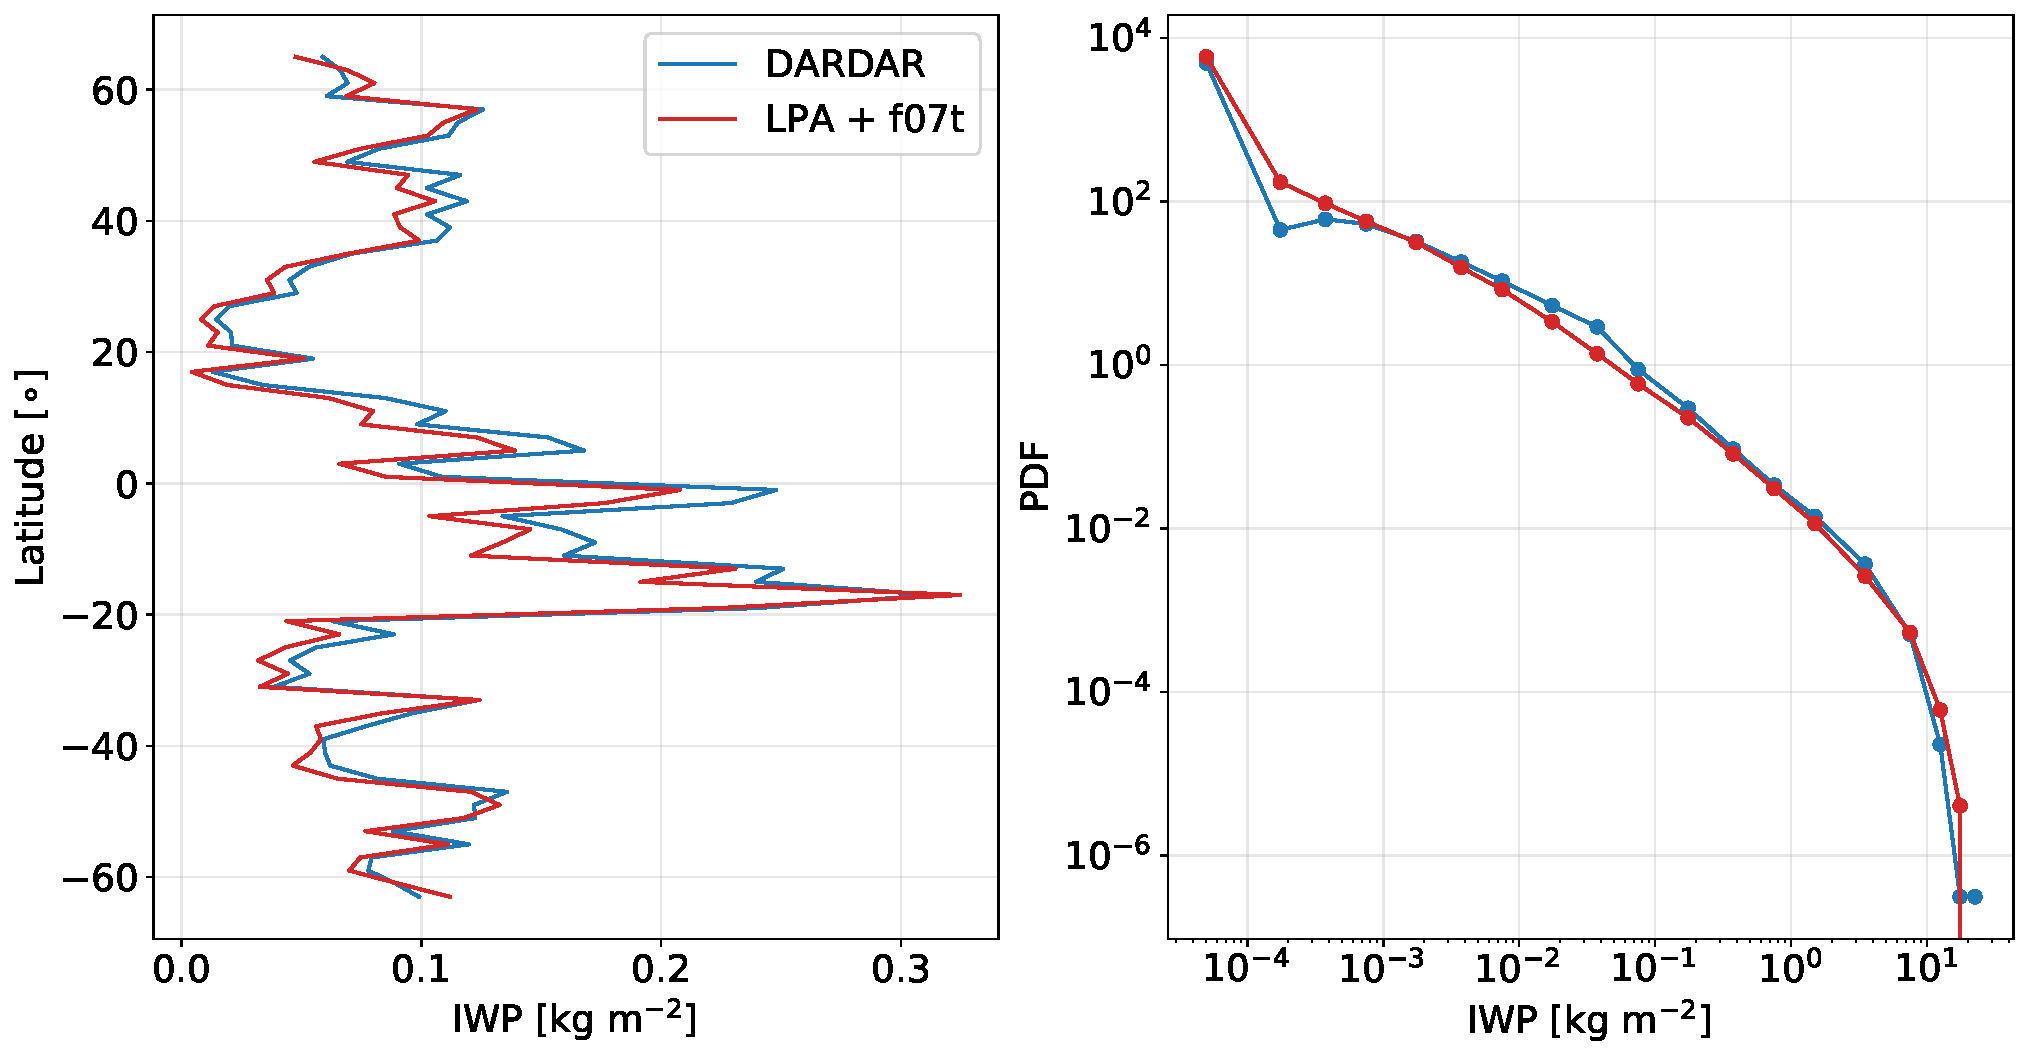
\includegraphics[width=6cm]{Figures/PDF_IWP_DARDAR.pdf}
	\caption{The zonal means (left) and  PDF of  the IWPs retrieved by inverting Cloudsat reflectivties and  DARDAR retrievals. The assumed particle habit is large plate aggregate.}
	\label{fig:IWP_DARDAR}
\end{figure}
\begin{figure}[t]
	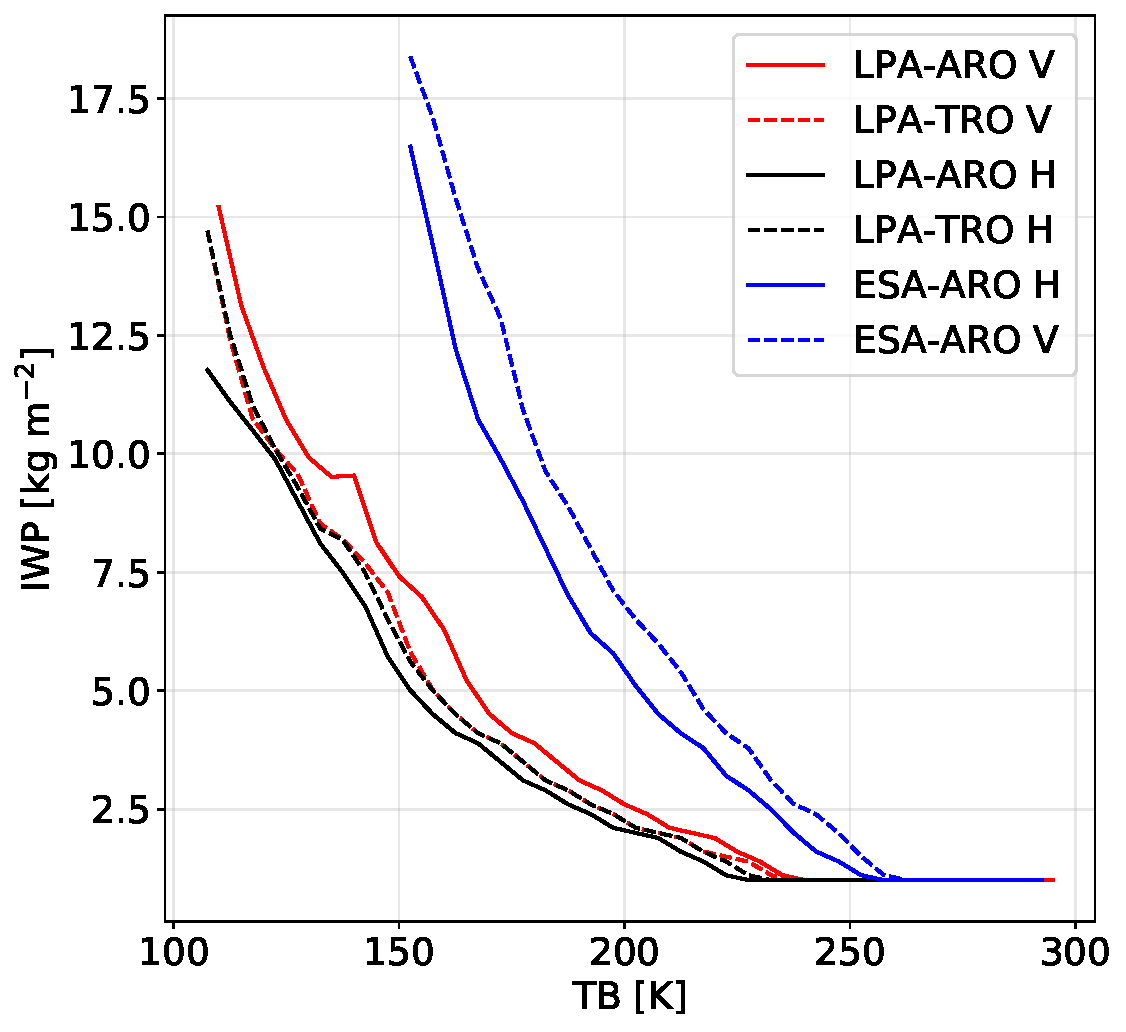
\includegraphics[width=4cm]{Figures/TB_IWP.pdf}
	\caption{TBs as a function of IWP at 166V and 166H\,\,GHz channels. The labels ``ARO V'' and ``TRO V'' refer to the V-polarisation with ARO particles and with TRO particles, respectively. Similarly, ``ARO H'' and ``TRO H'' refer to the H-polarisation. The results are from large plate aggregate.}
	\label{fig:TB_IWP}
\end{figure}

For any ML retrieval to work efficiently, the training data should reflect the realistic scenarios as close as possible. In this study, since we do not use any collocated datasets, the IWP is calculated by inverting the Cloudsat reflectivties. This is explained in detail in \citet{ekelund2020using}, but for completeness, we provide a comparison of the IWPs inverted from dbZ with the actual DARDAR IWPs (Fig.~\ref{fig:IWP_DARDAR}). Overall, the radar inversions agree
fairly well with the DARDAR IWPs, however the zonal means can be upto 16\% smaller than DARDAR.  his can be explained by two reasons. Firstly, DARDAR retrievals include lidar measurements which are sensitive to thin ice clouds. Lack of such measurements in our inversions leads to lower IWCs at high altitudes (where thin cirrus clouds are abundant) as compared to DARDAR. Secondly, the assumed microphysical set-up has a strong affect on the dbZ inversions. \citet{ekelund2020using} provides a detailed analysis on this aspect.

Fig.~\ref{fig:TB_IWP}, which displays the peak probability density of the two-dimensional histogram between TB and IWP. For TRO particles, the differences between the V- and H- polarisations (or PD) are close to zero except for IWPs < 2\,\,kg m$^{-2}$, which occur due to the impact of surface emissions. However, for ARO particles, the PD are positive. This is due to the dichroism effects exhibited by scattering from horizontally oriented ice particles. As IWP increases, the TB depressions become more prominent, for example, or IWP around 6\,\,kg m$^{-2}$ the PD is around 25\,\,K. But the PD do not increase drastically with an increase in the IWPs, but instead, a saturation in the PD is seen. TB distributions with evans snow aggregate are shown in Appendix~\ref{app:esa}.

\subsection{IWP retrievals}
%
\label{sec:iwp_retrievals}

\subsubsection{Retrieval experiments}
%
In order to scrutinize the impact of databases on the retrieval performance, two retrievals are performed: with and without orientation effects. A separate QRNN is trained for each of the two databases, that is, LPA-ARO and LPA-TRO(sect.~\ref{sec:database}). The basic construction of both trainings is identical (Sect.~\ref{app:qrnn_conf}), except for the input database each is based on. 

Furthermore, two additional QRNN trainings are considered. These two trainings are based on databases LPA-ARO and LPA-TRO, but the input data is slightly different. Here, instead of including both polarisation channels of 166\,\,GHz, only the V-polarised channel is included.

\subsubsection{Basic retrieval performance}
%
\label{sec:basic_performance}

\begin{figure*}[t]
	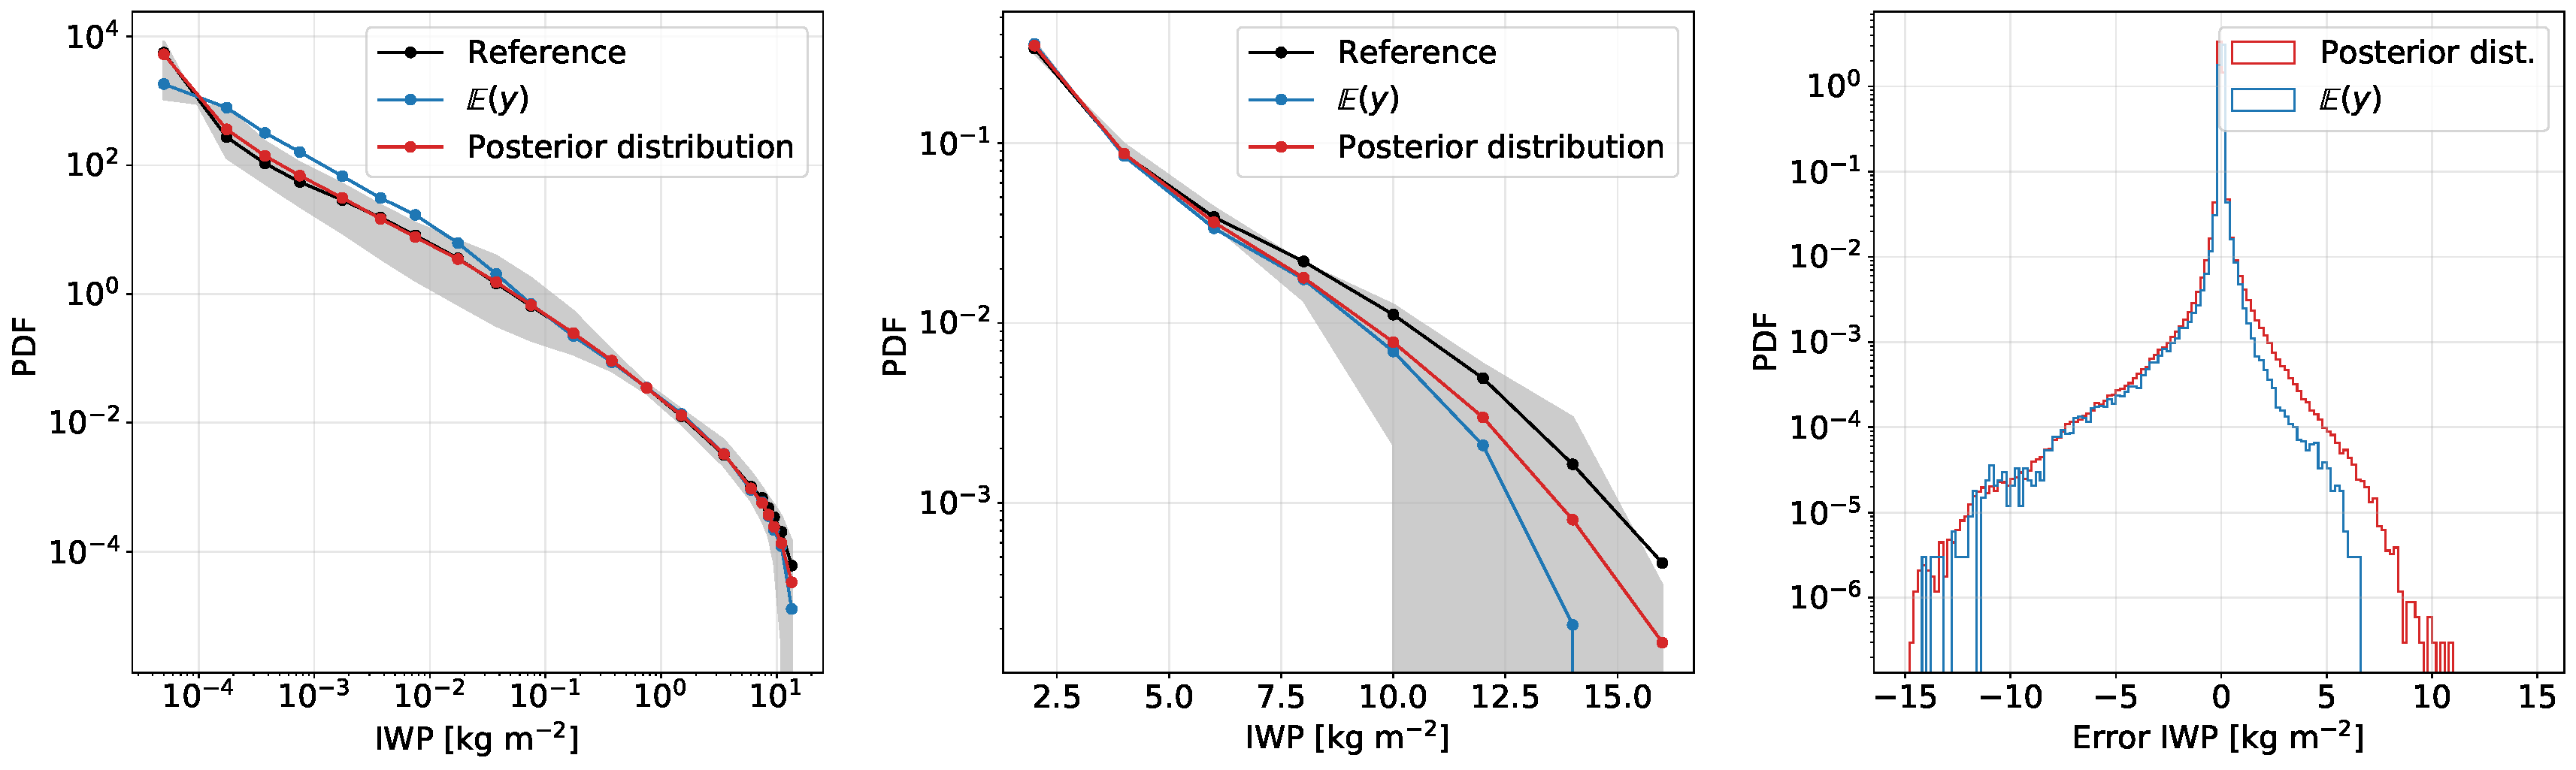
\includegraphics[width=12cm]{Figures/PDF_IWP_ARO.pdf}
	\caption{(a) The PDF of the retrieved and reference IWPs. The distribution of random samples drawn from the posterior distribution is shown in red. The point estimates of IWP retrieval are represented by the expectation value (blue). The shaded region represents the spread of the distribution bounded by 5\% and 95\%; (b) Same as (a) but a zoom in on the higher IWPs; (c) the error distribution. }
	\label{fig:PDF_IWP_test}
\end{figure*}

To evaluate the  retrieval performance of QRNN, retrievals on the test dataset are compared against the true state vectors. The test dataset is part of the LPA-ARO database, but not revealed to the network during training. It provides a way to check the model accuracy against the data that was not used in the training procedure. This is an idealised retrieval where both the training and test datasets have same underlying a priori distributions. As mentioned in sect.~\ref{sec:QRNN} the expectation value is taken as the point estimate. Further in the text, ``retrieved IWP'' always refers to this point estimate.

Figure~\ref{fig:PDF_IWP_test}(a) shows the normalised distributions of the observed and retrieved state vectors. The posterior distribution and the spread of the retrievals in the 90\% confidence interval (bounded by 5\% and 95\% quantiles) are also shown. The posterior distribution outputted by QRNN is of high interest here. It captures well the entire reference distribution, except the very high values above 10\,\,kg m$^{-2}$.  On the other hand, the expectation value has a different behaviour. For low IWPs (< 0.01\,\,kg m$^{-2}$) the occurrence frequency of retrieved IWPs is higher, while the very high IWPs (> 10\,\,kg m$^{-2}$) occur less frequently. For the intermediate IWP range, the dispersion in the 90\% confidence interval is quite low, thus the retrievals are  sharper and better calibrated. However, for the very low IWPs, the retrieved IWPs lie outside the 90\% confidence interval and are poorly calibrated. Overall, QRNN overestimates the low IWP values (thin ice clouds) and  slightly underestimates the larger IWPs (thick ice clouds).

A high degree of match between posterior and reference distribution confirms that QRNN can combine the information provided by a priori as well as the input data to output a well defined posterior. The low representation of the high values is likely due to under-representation of such cases in the apriori dataset. Any machine learning model is expected to learn about data from the a priori distribution and input data. Any missing information is always conditioned by the a priori. Ideally, an infinitely large database would be needed to provide for all under-representation, but in reality such databases are not feasible. Additional simulations can improve the representation and retrievals, but the complete information cannot be expected. 


Our retrievals are based on a transformed log-linear scale therefore the retrieval is always non-zero. Thus, to quantify the rate of missed  and false positive retrievals, we assume the cutoff IWP threshold for clear-sky conditions as 0.05\,\,kg m$^{-2}$. A false positive occurs when, the reference is lower than this threshold, but the retrievals are higher than 0.20\,\,kg m$^{-2}$, and vice-versa for the missed retrievals. In total, only 1.5\% of the clear-sky cases end up with false positives, and 0.20\% of the all-sky cases are missed. While in both cases, though the number of wrong retrievals is quite low, it seems to have a dependence on surface types. Interestingly, most false negatives occur for water and snow surface types and towards the warmer TBs (less than 190\,\,K at 166V GHz). For former, such cases are mostly concentrated at 275\,\,K and low values of PD.  However for snow surface type, missed retrievals are spread out over the entire range of TBs. Similarly, when QRNN falsely retrieves high IWP for clear-sky cases, most cases occur over water, but land and snow also account for around 25\% cases each. Such cases arise from the less represented part of the a priori distribution. Due to the scarcity of the observations in outlying regions of the state space, their quantiles are poorly calibrated. However, due to their low fraction, filtering these false retrievals has little effect on the performance on the basic accuracy. 




%\begin{figure}[t]
% 	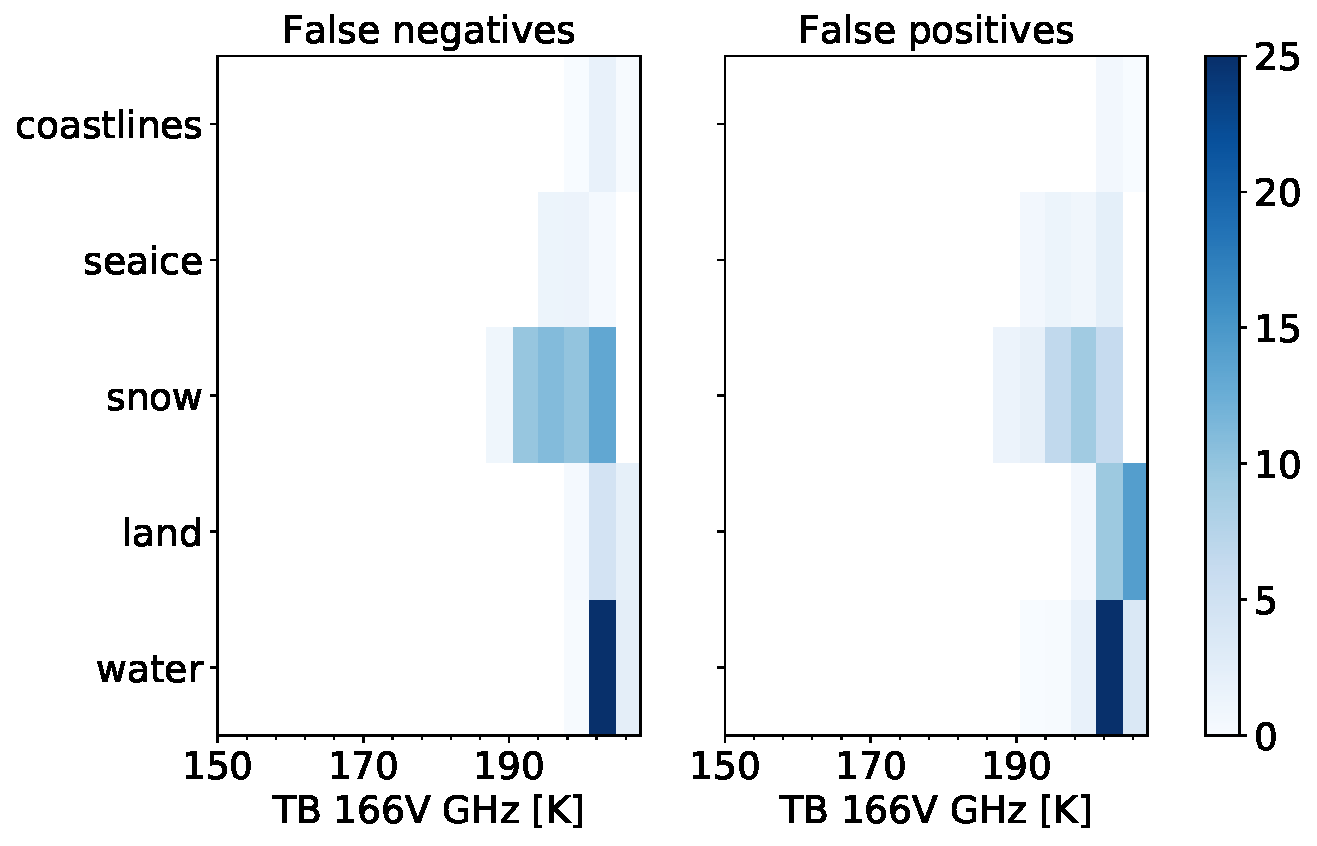
\includegraphics[width=8.3cm]{Figures/false_miss.pdf}
% 	\caption{The occurrence rate (in \%) for false negatives and false positives subset by the TB at 166V\,\,GHz and surface types. A false negative occurs when the retrieved IWP is greater than 0.20\,\,kg m$^{-2}$ and the reference is less than 0.05\,\,kg m$^{-2}$. While, a false positive occurs when the retrived IWP is less than 0.05\,\,kg m$^{-2}$ and the reference is greater than 0.20\,\,kg m$^{-2}$. }
% 	\label{fig:false_ret}
%\end{figure}  
 

\subsubsection{Impact of oriented particles}
\label{sec:impact_retrieval}
%
To examine the impact of oriented hydrometeors, we compare the IWP retrievals based on LPA-ARO and LPA-TRO databases. Though, LPA-TRO has a different a priori distribution than LPA-ARO, for an exact comparison, we use an identical test data (based on LPA-ARO). In this case, the retrievals based on LPA-TRO training will not reflect the true QRNN performance, but the same is also not expected. In an ideal world, a trained model is expected to make predictions using input data following the same underlying distributions, however for realistic situations this assumption can be violated due to many aspects not considered in the database. Similar is the situation with LPA-TRO database. This database lacks the contribution from oriented hydrometeors, but in reality, this effect cannot be neglected. Basing the comparison of LPA-ARO and LPA-TRO based trainings on a LPA-ARO test dataset, can help us to quantify the IWP errors introduced by neglecting polarised signals. The retrievals based on these trainings are denoted by the name of the database they trained on.

Two types of comparisons are made. Firstly, a comparison of the retrievals based on QRNN trained with both V- and H- polarised channels  is made. Secondly, a comparison of retrievals based on QRNN trained with only V- polarised channel is made. The retrievals from the latter two trainings are referred as LPA-ARO(V) and LPA-TRO(V) further in the text.  


\begin{figure*}[t]
	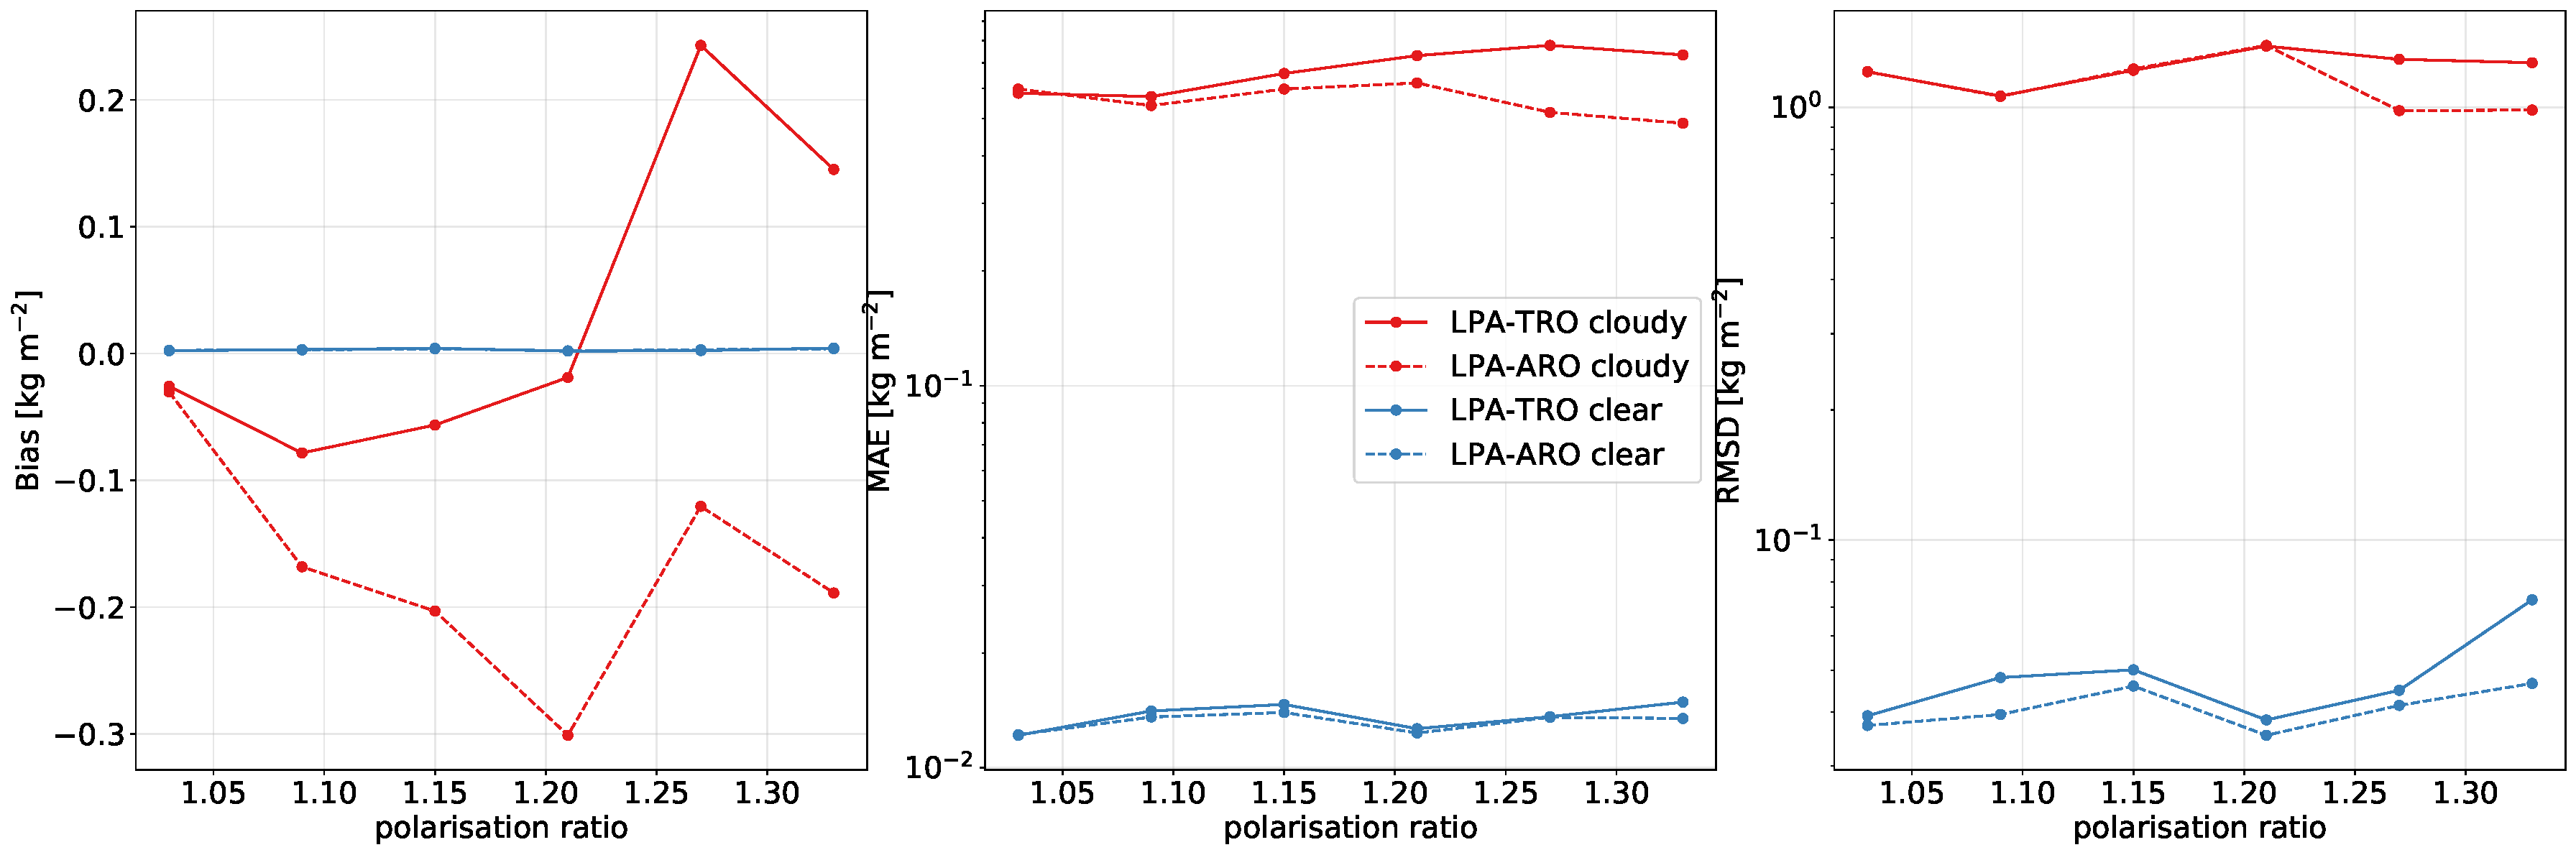
\includegraphics[width=12cm]{Figures/statistics_cloudyclear.pdf}
	\caption{Statistics showing the accuracy of retrieved IWPs
		binned according to the polarisation ratio ($\rho$). The red and blue curves represent cloudy data (IWP > 0.1\,\,kg m$^{-2}$
		clear data (IWP < 0.1\,\,kg m$^{-2}$) respectively.}
	\label{fig:clear_cloudy}
\end{figure*}

\begin{figure*}[t]
	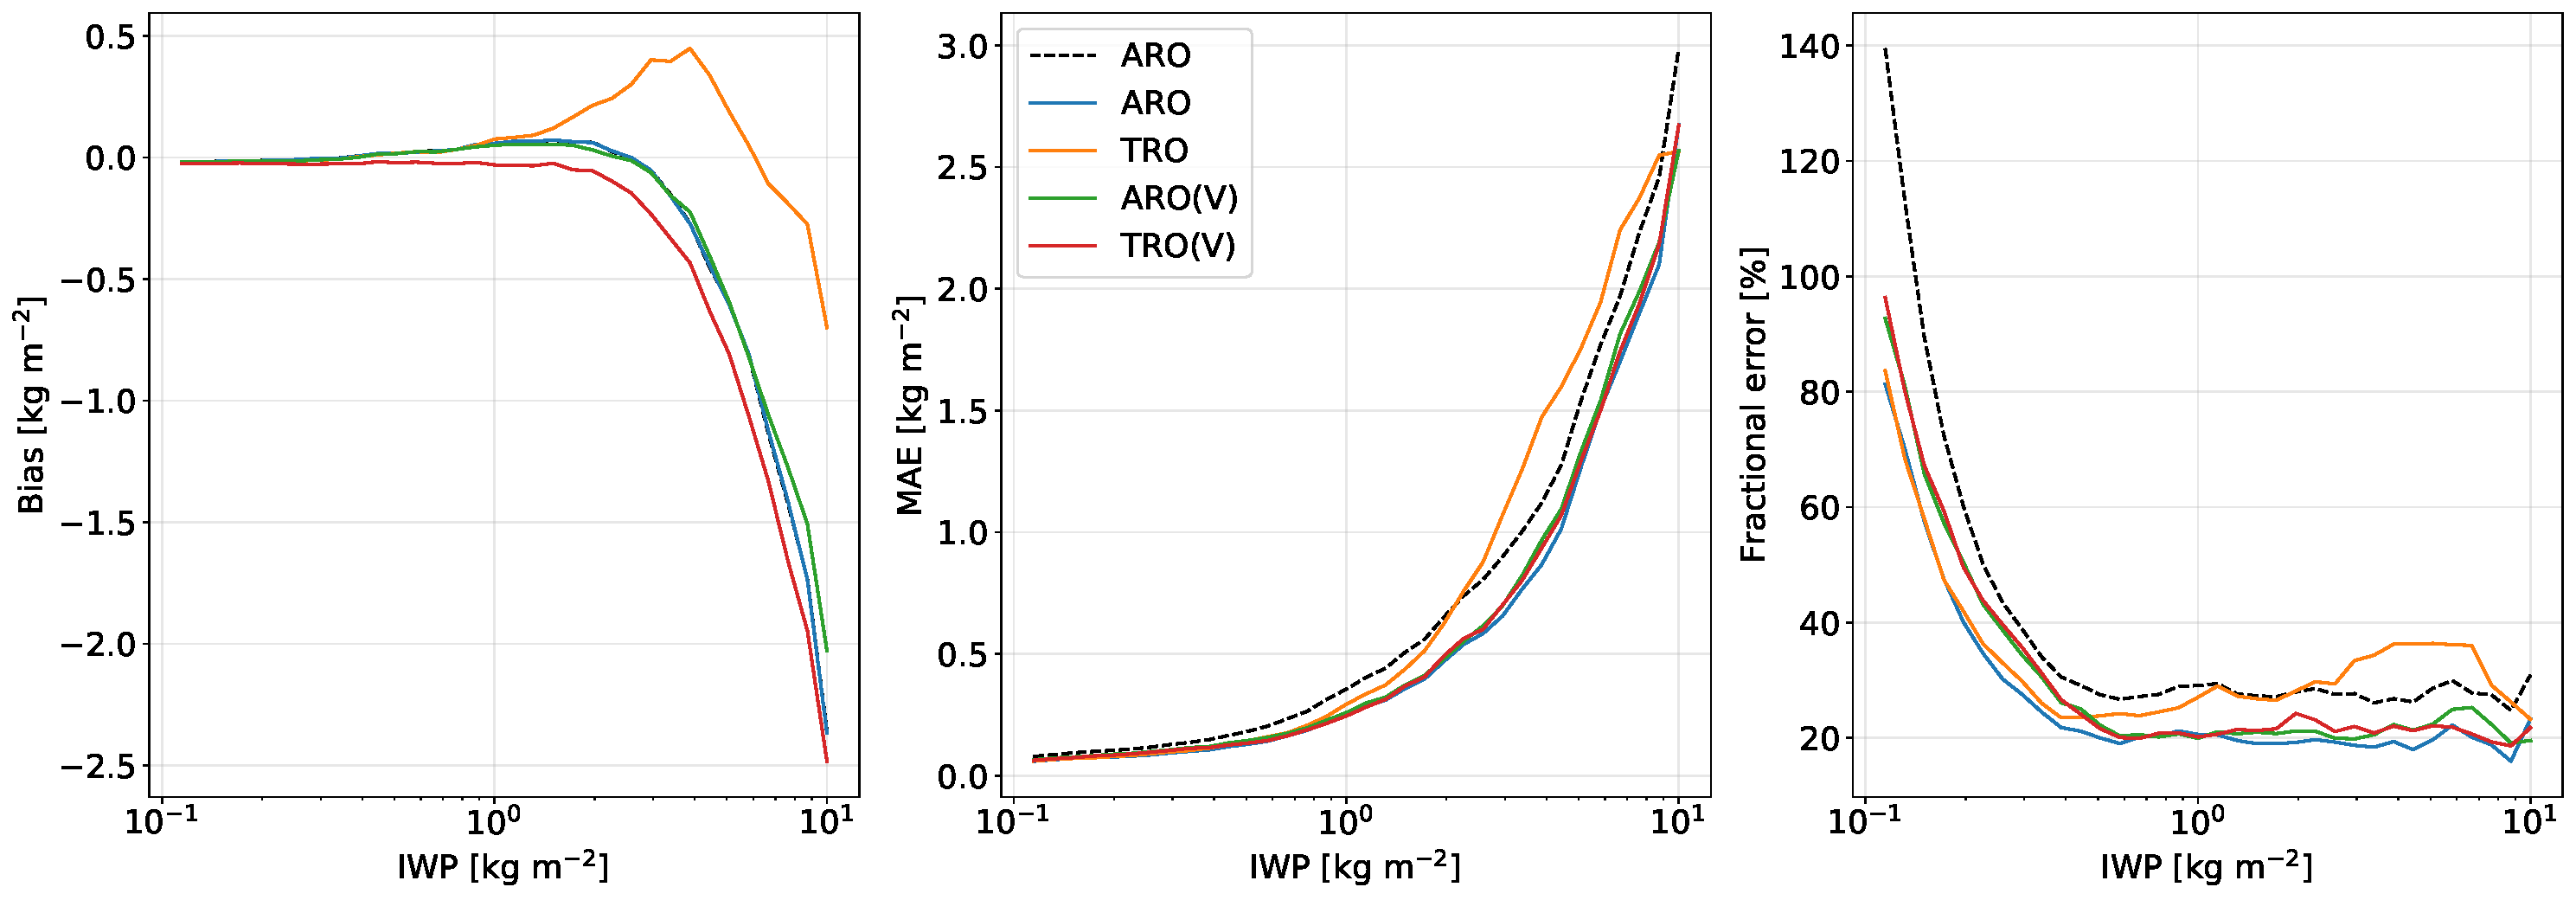
\includegraphics[width=12cm]{Figures/IWP_statistics.pdf}
	\caption{The bias, mean absolute error (MAE) and fractional error (FE) for binned according to IWP range. Results from four retrievals are shown: ARO and TRO refer to retrievals with and without particle orientation and with dual-polarised channels; ARO(V) and TRO(V) are similar to ARO and TRO but with only V-polarisation. }
	\label{fig:IWP_stats}
\end{figure*}



\begin{figure*}[t]
	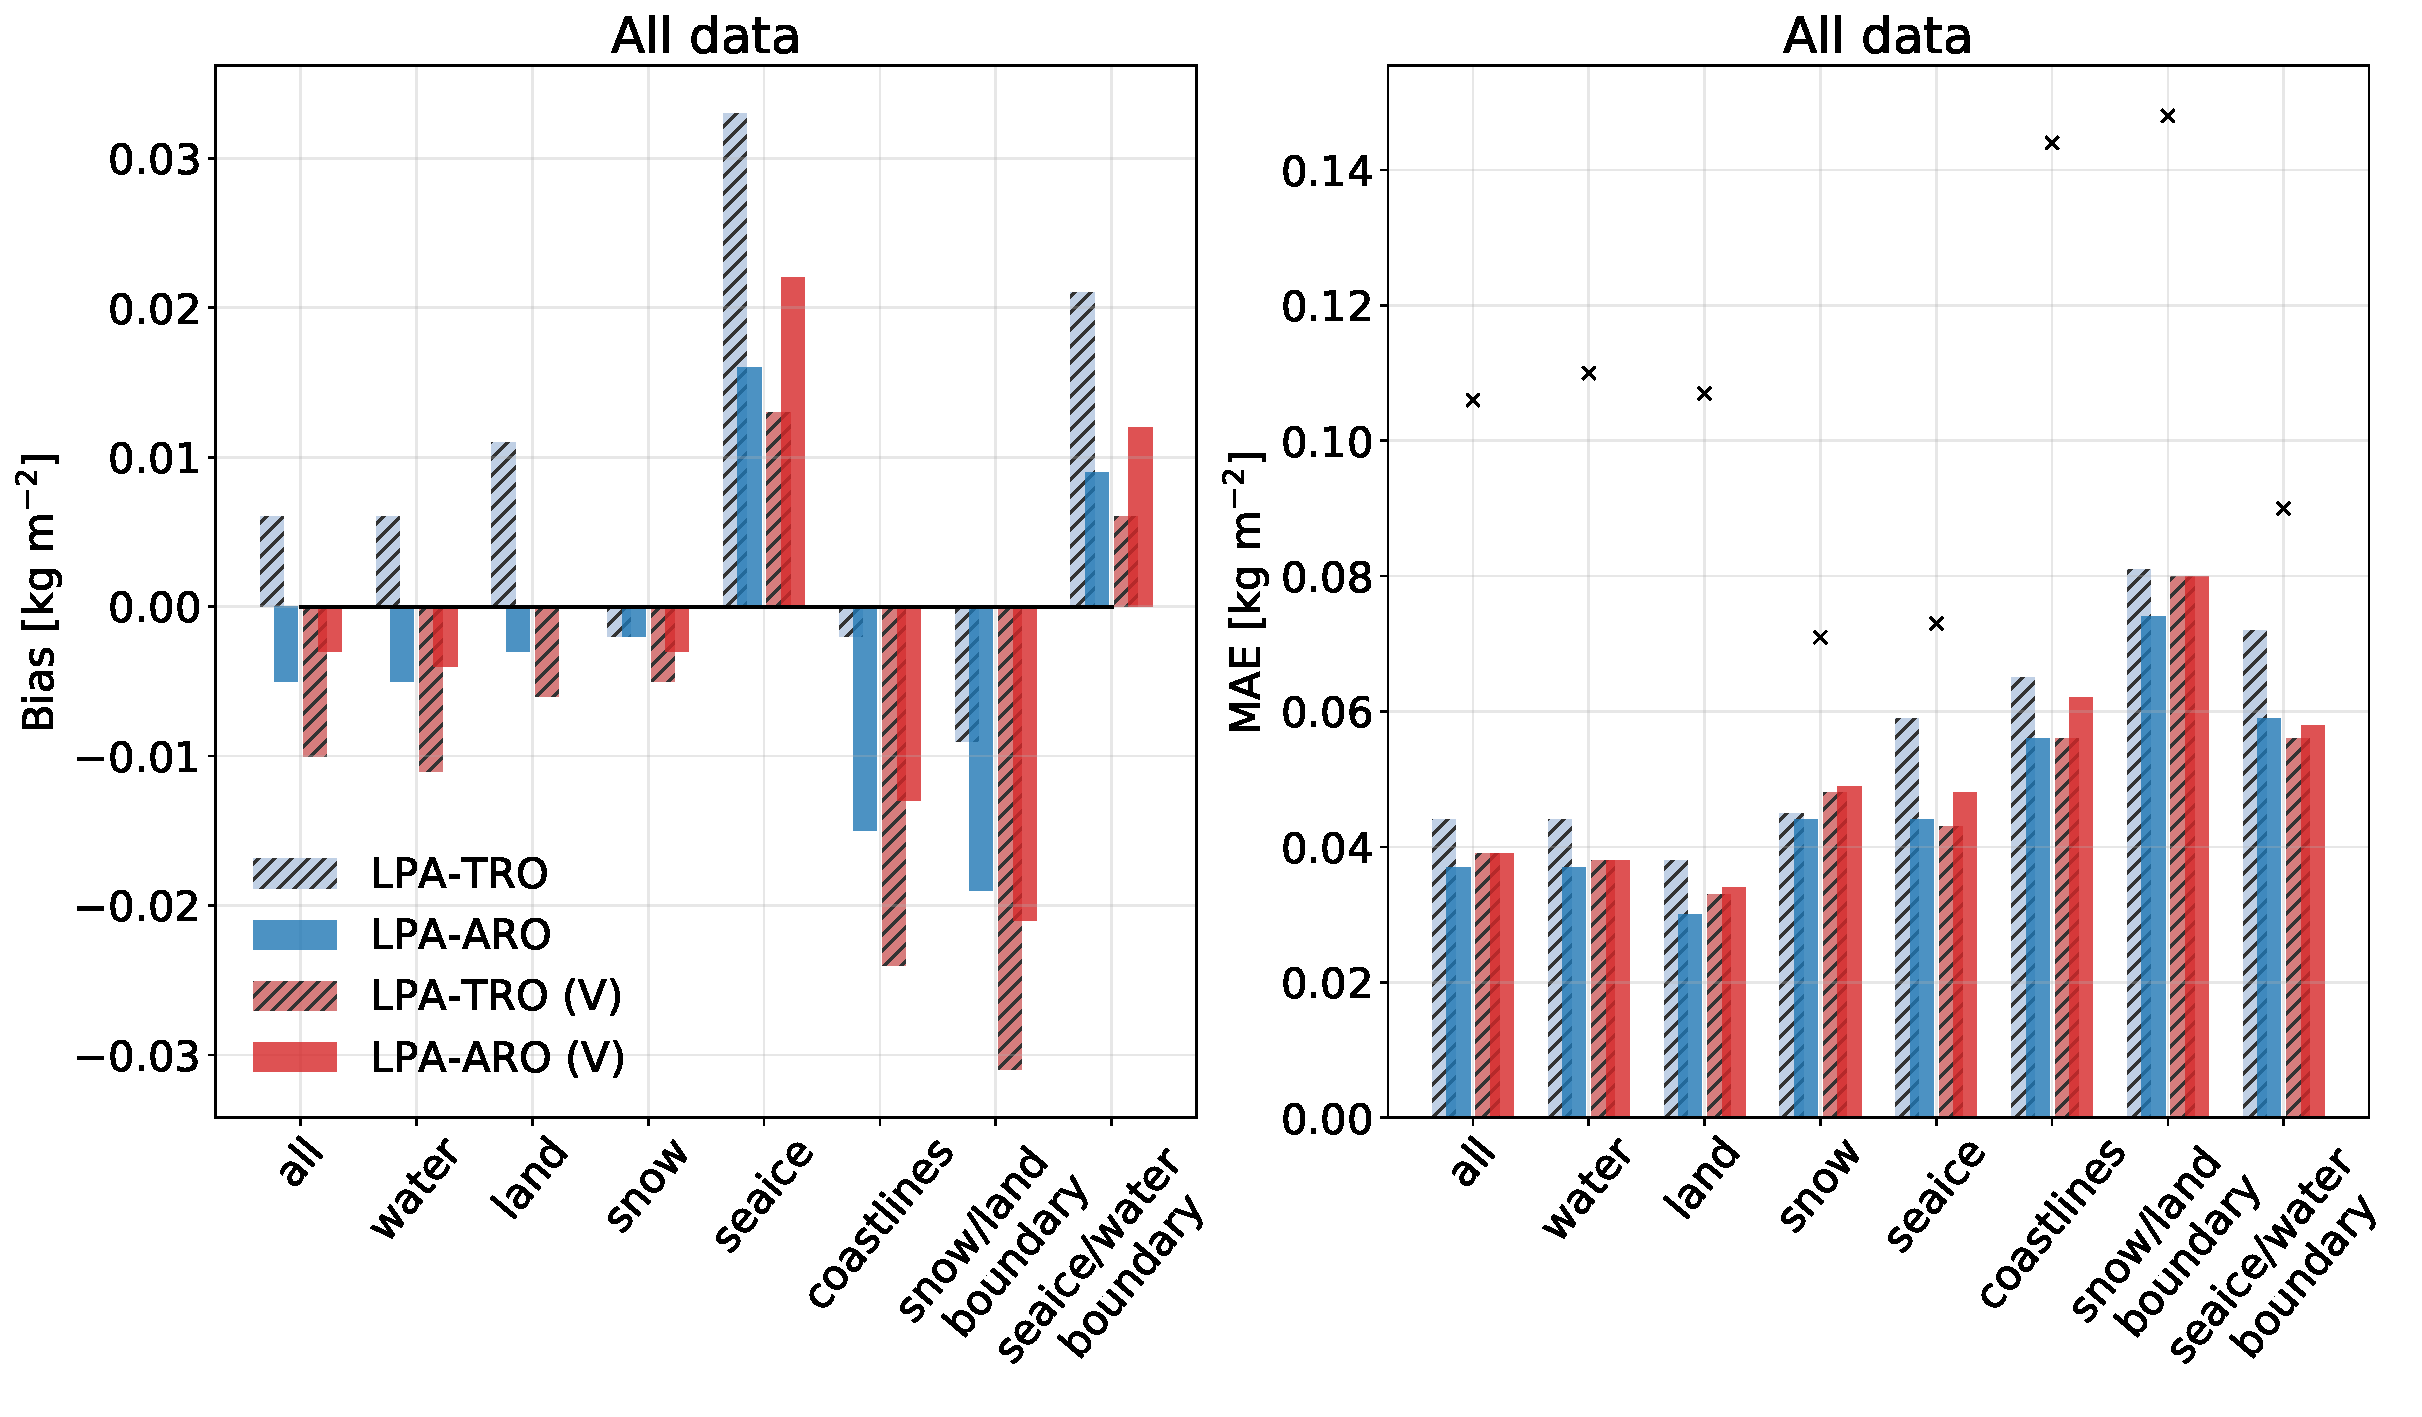
\includegraphics[width=10cm]{Figures/ARO_TRO_v_vh_all.pdf}
	\caption{A comparison of the IWP retrievals using ARO and TRO based databases. The results from four different retrievals are shown. The bars in blue show a comparison of retrievals when both V- and H- polarised channels are included in QRNN training. The bars in red show the comparison when only V- polarised channel is used. The black crosses in centre panel shows the mean of reference IWPs.  }
	\label{fig:bias_ARO_TRO}
\end{figure*}

\begin{figure}[t]
	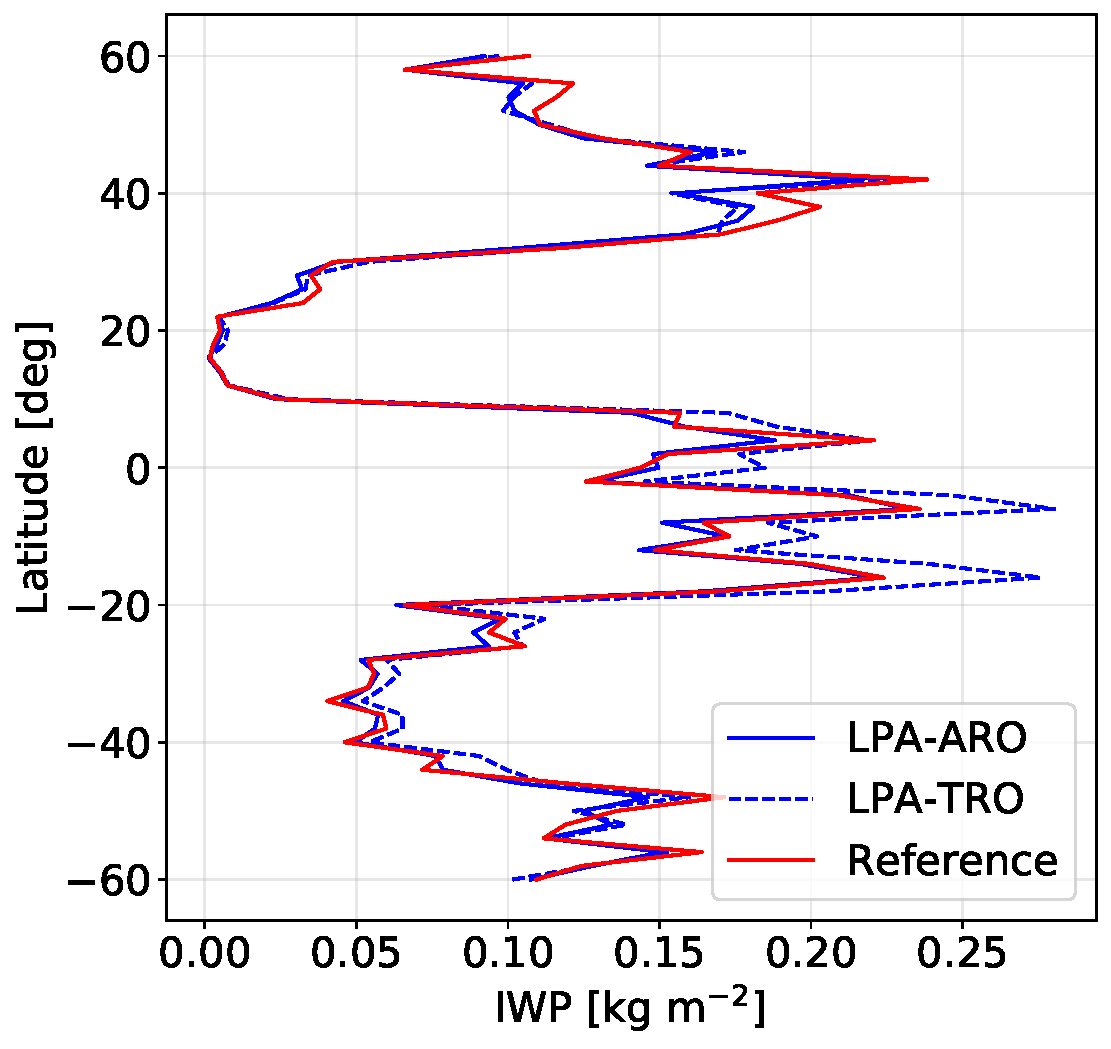
\includegraphics[width=6cm]{Figures/zonal_mean_all_jan_testdata.pdf}
	\caption{The zonal mean of reference and retrieved IWPs. Only the  IWP retrievals based on databases LPA-ARO and LPA-TRO are shown.}
	\label{fig:zonal_mean_test}
\end{figure}

Figure~\ref{fig:clear_cloudy} shows the error statistics for retrievals based on random orientation (LPA-TRO) and preferential orientation (LPA-ARO). The retrieved data has been binned according to $\rho$ and divided into cloudy and clear-sky based on the reference IWP.  All IWPs below 0.01\,\,kg m$^{-2}$ are classified as clear-sky, and vice-versa. The clear-sky IWPs can also have contribution from thin cirrus clouds. For clear sky cases, $\rho$ has a negligible impact on the accuracy of the retrievals. The IWPs in this range are slightly overestimated as indicated by the low positive bias. On the other hand, for cloudy cases, a strong dependency of the accuracy on $\rho$ is observed. For $\rho = 1$ the both retrieval sets have similar accuracy. As $\rho$ increases up to 1.2, the bias in LPA-TRO is lower than LPA-ARO, but MAE shows slightly better accuracy for LPA-ARO. At the same time, RMSD remains unchanged between the two. However for $\rho > 1.20$, the differences between the two retrievals are quite prominent. The bias increases from -0.04 to 0.03 for $\rho = 1.35$, indicating an increase in the magnitude of IWP retrievals. This overestimation reduces the accuracy as indicated by the MAE and RMSD values. For $\rho = 1.35$ the RMSD increases by almost 25\%. This is  not totally unexpected as this part of the distribution represents maximum PDs due to hydrometeor scattering, and cannot be represented assuming a priori distribution based on random orientation. Overall, neglecting oriented particles leads to an overestimation of the IWP. 


Figure~\ref{fig:IWP_stats} shows the bias, MAE and FE between the retrieved and reference IWP. Only IWPs > 0.1\,\,kg m$^{-2}$ are considered here. Retrievals with only V-polarisation are also shown.  Below 0.1\,\,kg m$^{-2}$, all four retrievals have quite low bias, but above for higher IWPs, the negative bias increases with increasing IWPs. Among the two retrievals with dual-polarisation, assuming random orientation (TRO) gives retrievals which are larger in magnitude than the reference. Above 1\,\,kg m$^{-2}$, the MAE is almost 1.7 times larger than retrievals assuming orientation (ARO). When only V-polarisation is considered, the retrieval with random orientation has lower bias than the retrieval with orientation upto 2\,\,kg m$^{-2}$. 
The FE larger is than 200\% for low IWPs (not shown), but for IWP > 0.1\,\,kg m$^{-2}$ it drops rapidly from 100\% to almost 20\%. This is better than the accuracy achieved by SpareIce IWP retrievals. SpareIce product is the column integrated bulk mass of ice and is retrieved as a combination of microwave, optical and infrared sensors. With only microwave channels, \citet{holl:spare:14} achieved around 100\% FE for very thick clouds with IWP of order of 1.0\,\,kg m$^{-2}$). When input data from infrared and optical sensors is added, the FE is around 50\%. Another comparison can be made with the snow water path retrievals attempted by \citet{brath:ismar:18} using sub-mm sensors. For IWP > 0.1\,\,kg m$^{-2}$, the FE is around 20\%. These comparisons are in no way a measure of the accuracy of our retrievals but are provided to get an estimate of what accuracy do other retrievals achieve.

Figure~\ref{fig:bias_ARO_TRO} (blue barplots) shows the bias and MAE values for these two retrievals for different surface types. Overall, the total bias between reference and retrievals is 0.006\,\,kg m$^{-2}$. While the overall trend is that LPA-ARO retrieves lower IWPs, but this is not true for the entire range. This performance is driven by the retrievals in the range IWP > 0.5\,\,kg m$^{-2}$. For very low IWPs ( < 0.01\,\,kg m$^{-2}$), the performance of both retrievals is almost identical. In this range, the bias and MAE have almost similar values, which reflects overestimation of very small values. This is in accordance with the basic retrieval performance described in sect.~\ref{sec:basic_performance}. In the intermediate range (0.01\,\,kg m$^{-2}$ >IWP 0.5\,\,kg m$^{-2}$ > ), both retrievals are lower in magnitude than the reference, but LPA-ARO are closer to the reference as indicated by the 15\% and 11\% reduction in the MAE and RMSD respectively. 

The retrievals over water and land drive the overall accuracy, due to their larger representation. However, for other surface types, varying accuracy is observed. Over coastlines, performance of the two retrievals is quite different. While the retrievals from LPA-TRO are bias free, the errors are higher in comparison to LPA-ARO. Over snow surface type, both retrievals have a comparable performance. The overall retrievals seem bias free but the MAE is almost 60\% of the mean IWP. This could be due to an increased frequency of both false positives and negatives, that is retrieval of non-zero IWP for a clear case and vice-versa. For seaice and seaice/water boundary, both retrievals are larger than the reference and the average bias in LPA-TRO is twice as higher than LPA-ARO. The overestimation of IWPs is observed over the entire dynamic range of IWP, but for the seaice boundary, most LPA-TRO retrievals associated with clear-sky/low IWP have an overestimation.
%In general, retrievals where dual-polarised observation of particle orientation are included, almost similar performance for clear-sky/thin cloud cases is observed.

Figure~\ref{fig:bias_ARO_TRO} (red bar plots) also shows the statistics for LPA-ARO (V) and LPA-TRO (V) based retrievals, that is, when only V-polarised channels is used. For all surface types except seaice and seaice/water boundary, including oriented particles reduces the negative bias in IWP retrievals. While the low range IWP retrievals between the two are comparable, for the intermediate and high IWP range, LPA-ARO(V) retrievals have lower bias values. For land and water, the bias is less than up to 50\%. These results are in contrast to the retrievals based on dual-polarised channels, where neglecting the oriented particles leads to an increased positive bias.


Figure~\ref{fig:zonal_mean_test}) gives an overview of the zonal averages from both retrievals. With ARO and dual-polarised channels, the overestimation is largest over the tropics, where most ice clouds exist, but over higher latitudes, in both hemispheres, the differences between the two are small. This is interesting because snow and seaice had comparatively lower accuarcy than water and land, but IWP mean over Northern latitudes is quite similar to DARDAR. This also shows that while the point estimates could have high error, the overall posterior can be estimated with high accuracy. 



\subsection{Retrieval applied to GMI measurements}
\label{sec:IWP_GMI}

\begin{figure}[t]
	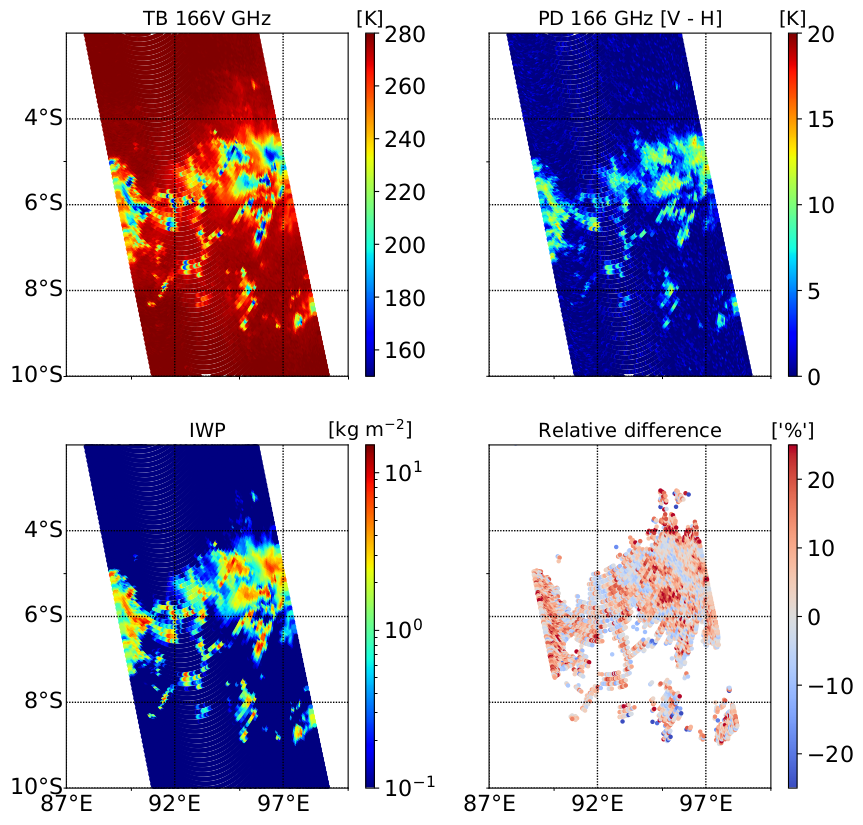
\includegraphics[width=6cm]{Figures/example1_tropics_gmi.png}
	\caption{ An example convection system observed by GMI on 15 January 2017. The top two panels show the observed TBs at 166V\,\,GHz and the PD between the dual-polarised channels (166V - 166H). The bottom left panel shows the retrieved IWPs when oriented particles are considered, while the right panel shows the relative differences from the IWP retrievals where orientation is neglected. The relative differences for clear-sky regions are masked.}
	\label{fig:example1_GMI}
\end{figure}

%\begin{figure}[t]
%	\includegraphics[width=6cm]{Figures/example2_gmi.pdf}
%	\caption{ Same as Fig.~\ref{fig:example1_GMI}, but for bottom left shows GOES infrared radiances (channel 16) and bottom right shows the IWP retrievals.}
%	\label{fig:example2_GMI}
%\end{figure}



\begin{figure}[t]
	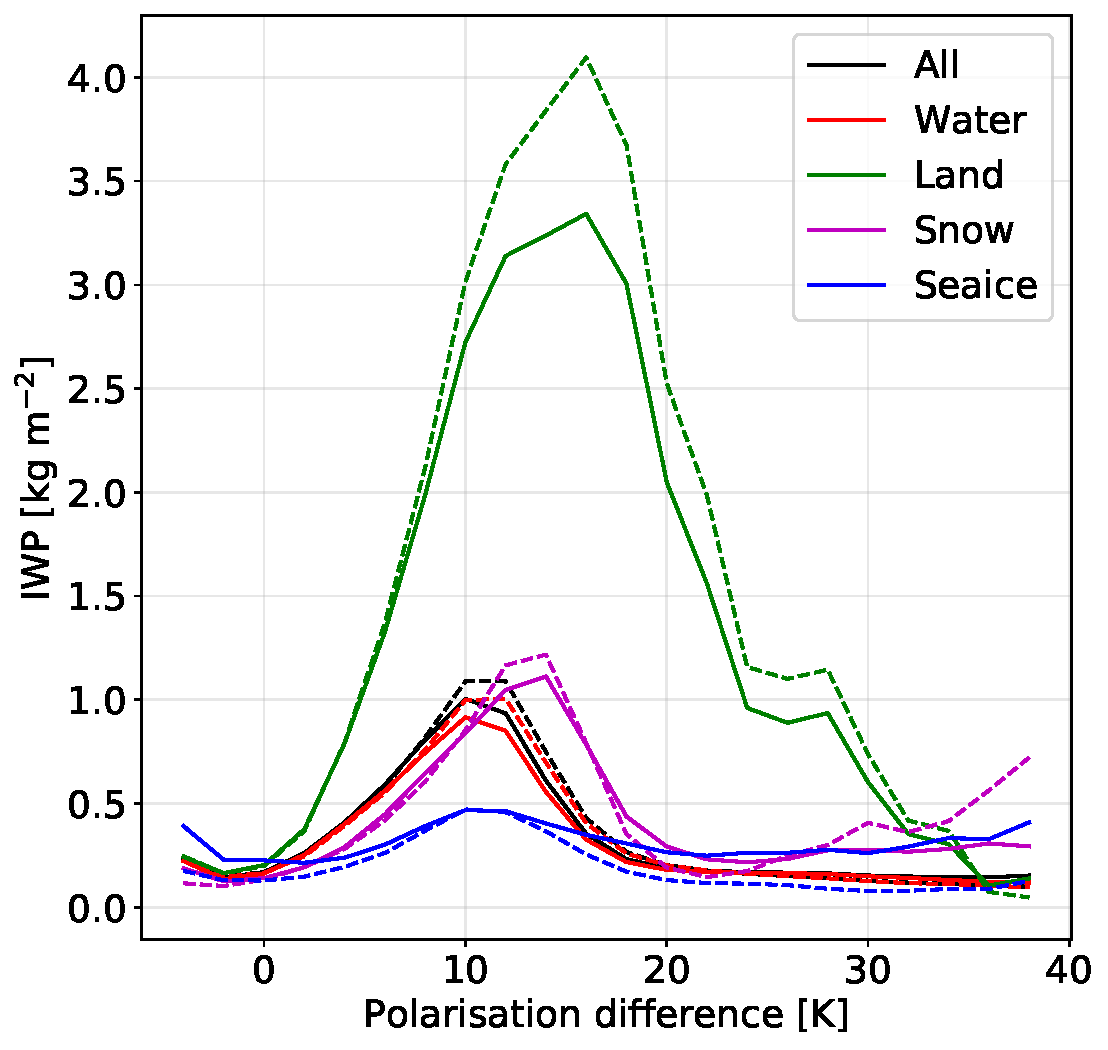
\includegraphics[width=4cm]{Figures/IWP_PD_GMI.pdf}
	\caption{ The average IWPs  from two retrieval datasets binned according to the polarisation differences. Four surface types are shown. The dotted lines denote the retrievals where ice hydrometeors are assumed TRO and the solid lines denote the retrievals where ARO particles are included. }
	\label{fig:IWP_PD_GMI}
\end{figure}



\begin{figure}[t]
	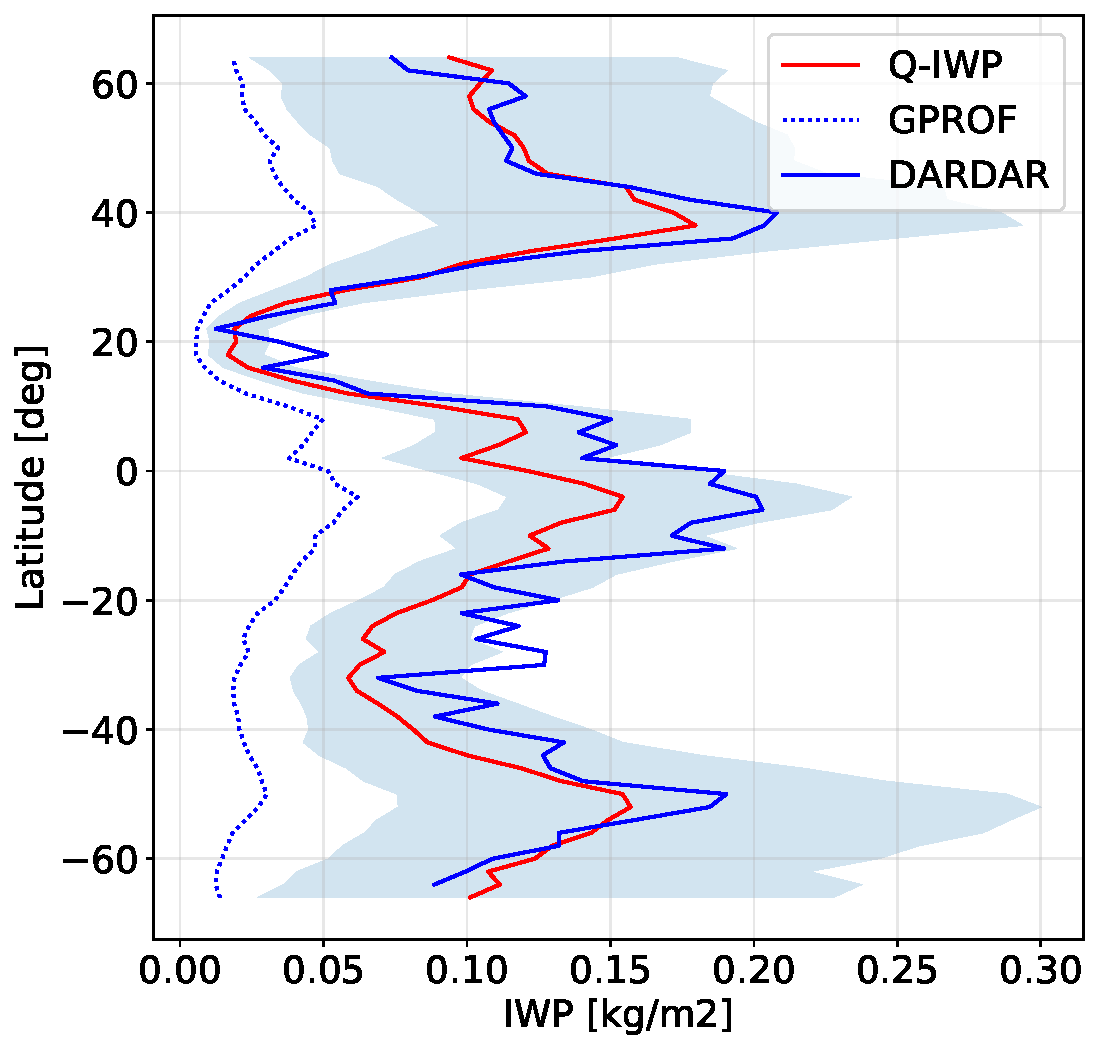
\includegraphics[width=4cm]{Figures/zonal_mean_jan_2017.pdf}
	\caption{ The zonal means of Q-IWP, GPROF and DARDAR observations for January 2017. The shaded area indicates the spread of retrieved IWPs in the 5\% and 95\% confidence interval. For DARDAR only daytime observations are considered.  }
	\label{fig:zonal_mean_GMI_17}
\end{figure}

%\begin{figure}[t]	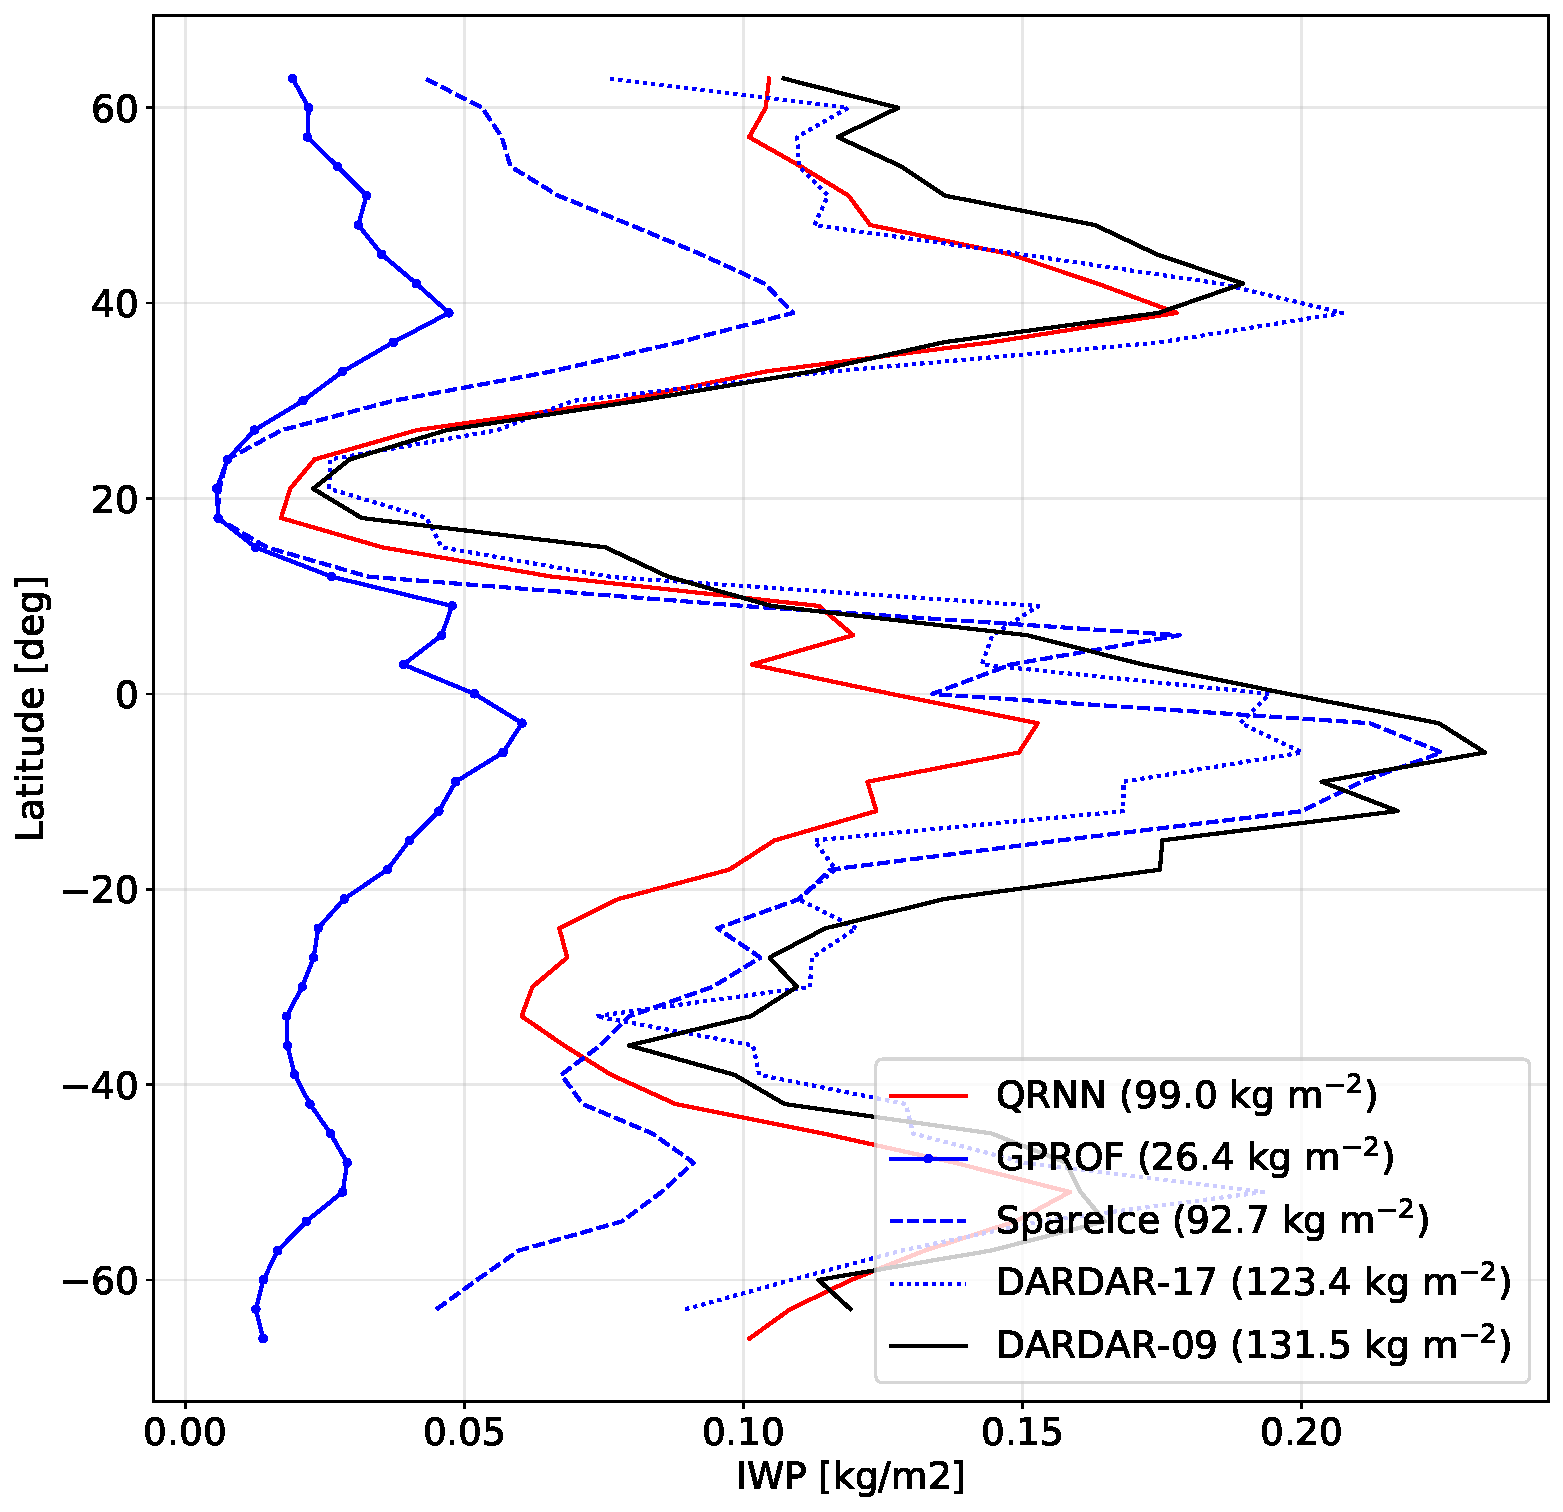
\includegraphics[width=6cm]{Figures/zonal_mean_all_jan.pdf}
%	\caption{Same as Fig~\ref{fig:zonal_mean_GMI_17}, but DARDAR observations from 2009 and Spare Ice obervations from 2013 are added for a qualitative comparison.}
%	\label{fig:zonal_mean_GMI}
%\end{figure}

\begin{figure*}[t]
	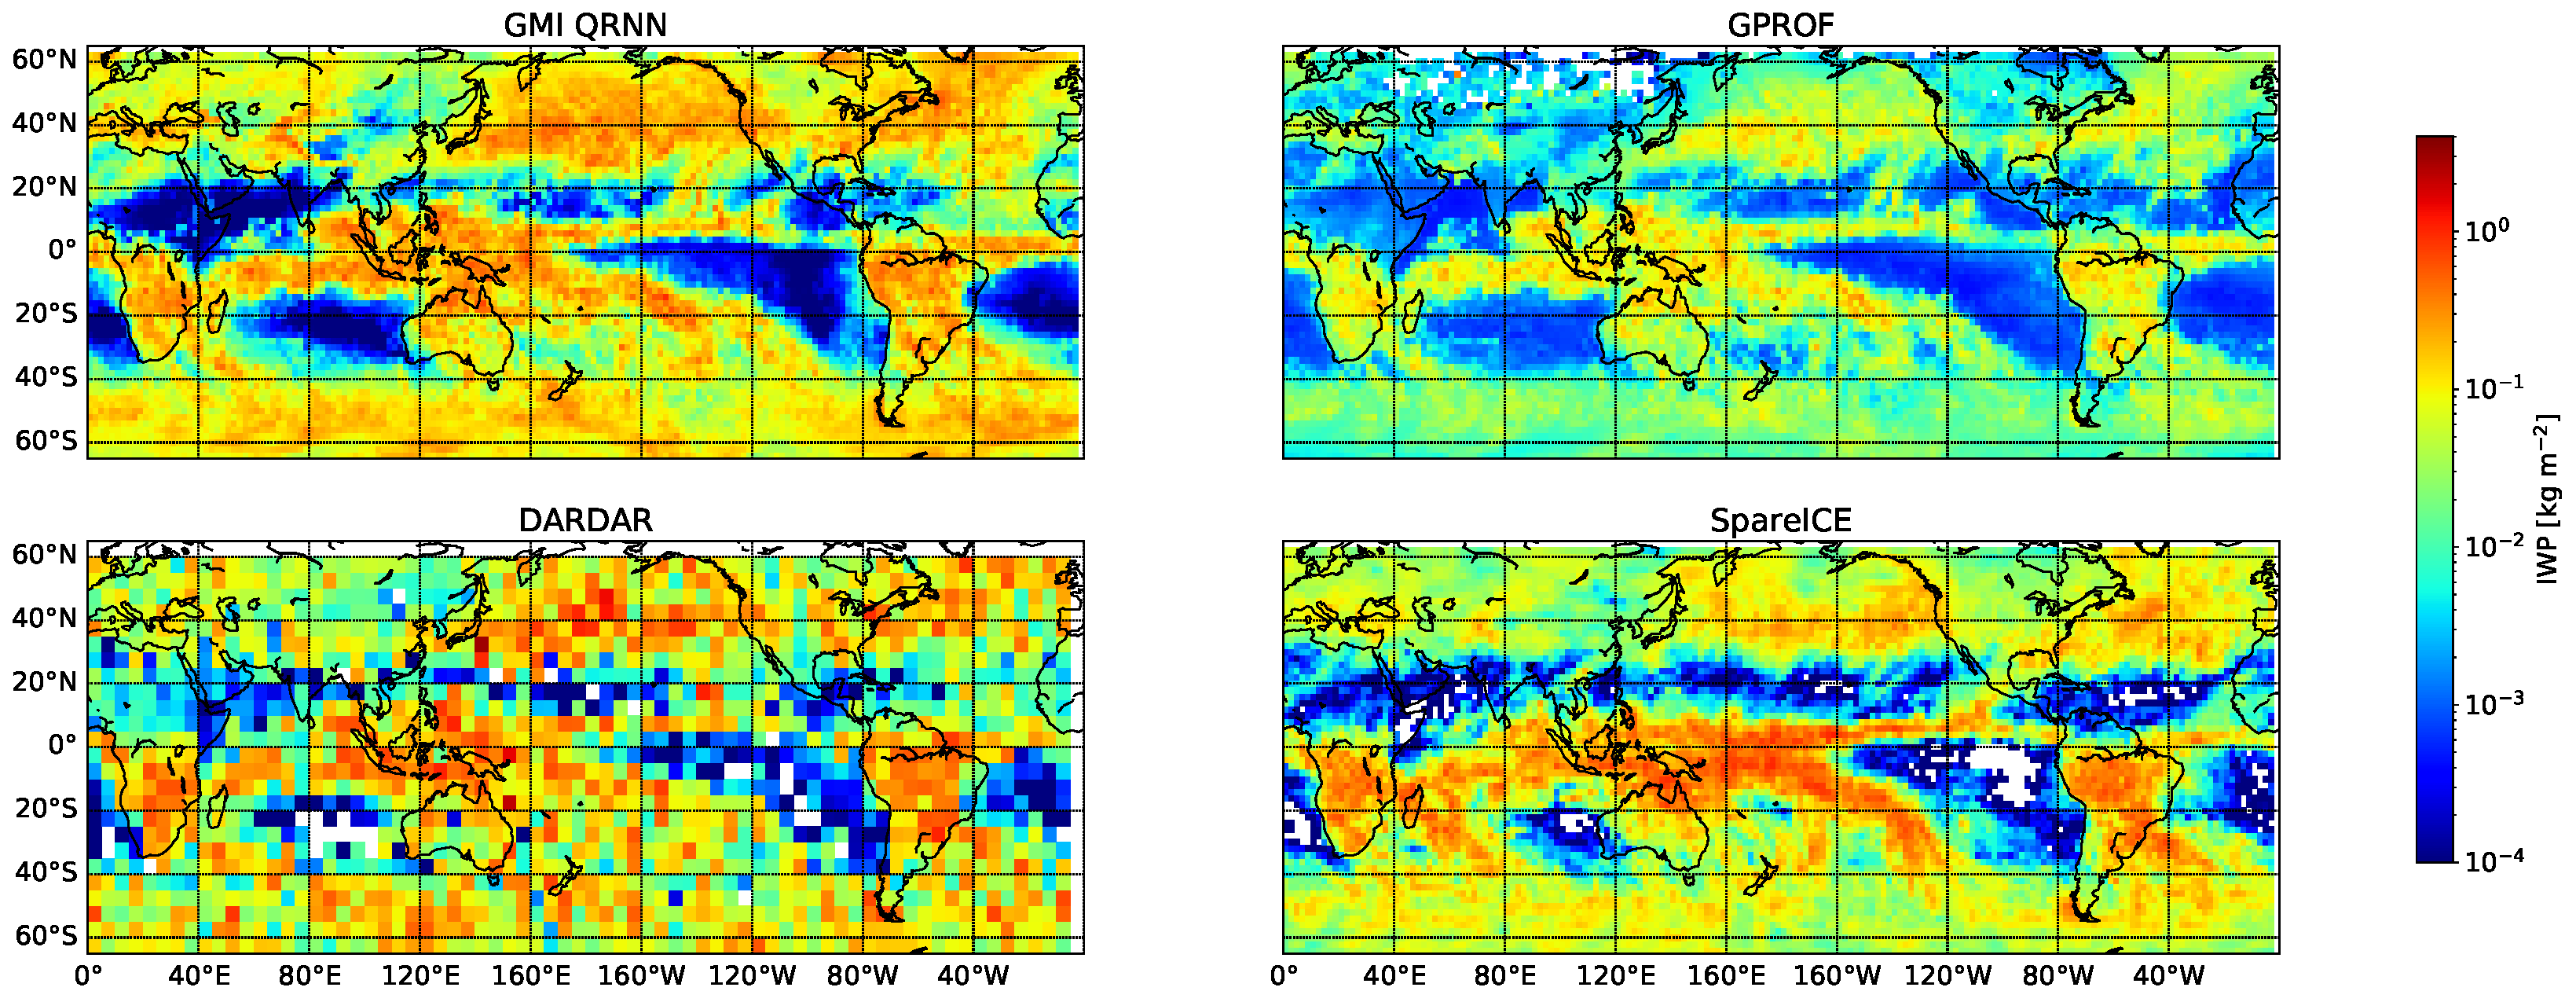
\includegraphics[width=16cm, height = 8cm]{Figures/IWP_spatial_distribution.pdf}
	\caption{ The gridded mean of IWP observations for QRNN retrievals, GPROF, DARDAR and SpareIce. DARDAR is gridded at 5$^\circ$ grid, while the other three datasets are gridded on 2$^\circ$ grid. }
	\label{fig:spatial_dist_GMI}
\end{figure*}

To show the performance of the retrieval algorithm on real measurements, GMI data from January is selected. In the absence of a reference for benchmarking these results, we show an example scene for a qualitative analysis. Figure~\ref{fig:example1_GMI} shows a convection system in the tropical Indian Ocean and the corresponding TBs at 166V GHz, PDs and the retrieved IWPs using LPA-ARO database, i.e. assuming oriented particles. The relative difference from retrievals asssuming TRO particles is also shown. The relative differences are masked for clear-sky areas with IWP < 0.05 kg m$^{-2}$. In the scene, the scattered convection activity has high PDs in the centre which tend to decrease towards the edges. The retrieved IWPs match quite well with the observed TB and PD signatures. The retrieved IWPs are maximum around the convection centres and decrease monotonically as the distance from the centre increases. The maximum retrieved IWP in this region is greater than 10\,\,kg m$^{-2}$. However when particle orientation is neglected, the retrievals are higher in magnitude as seen by the positive relative differences. The IWPs along the convective activity can be around 20\% higher. While we do not have any reference value to compare which one is more accurate, but these results are in conformity with the test retrievals described in  Sect.~\ref{sec:impact_retrieval}.

% In the second example (Fig.~\ref{fig:example2_GMI}) we show a retrievals over a system in the high latitudes. The corresponding GOES-16 infrared (IR) radiances at 13\,\,$\mu$m are also shown. The land area around 55$^{\circ}$ is dominated by low TBs around 200\,\,K, and the corresponding PDs are around 10\,\,K. This area is covered with snow and despite the low  TBs our algorithm retrieves almost negligible IWPs. This is confirmed by the visual inspection of IR radiances, which show almost nil cloud cover. However, over water, IWPs > 0.1\,\,kg m$^{-2}$ are retrieved, which is confirmed by the presence of thin clouds in the IR radiances. 

While the this example can provide an idea of how the two retrievals differ, it is not sufficient to describe the global differences. Figure~\ref{fig:IWP_PD_GMI} quantifies the average IWPs from both retrievals for different PDs bins. IWPs with magnitude less than 0.001\,\,kg m$^{-2}$ are not included in these statistics. For PDs < 10\,\,K both retrievals are quite similar and the differences are of the order of 1-2\%. These could also be due to retrieval uncertainties. However as PD increases, neglecting random orientation leads to around 20\% higher retrievals overall. For land, the maximum differences (27\%) occur 22\,\,K PD, while for water the two retrievals differ by 25\% around 14\,\,K. For PDs resembling the effects of surface emission, differences between the two retrievals are negligible for water and land. For snow and seaice differences are also observed for PD > 20\,\,K.  Such cases are few and as shown in Sect.~\ref{sec:comparison_sim_obs}, the cases with high PD mostly belong to mix surface types, which could have high probability of misclassification.


Figure~\ref{fig:zonal_mean_GMI_17} shows the zonal means for our retrievals, GPROF and DARDAR retrievals from the same period. While the overall shape of the zonal means is consistent with the southern hemisphere summer, but there is a lack of agreement among the magnitudes. GPROF IWPs are too small, but our retrievals match quite well with DARDAR magnitudes especially over the high latitudes. However, they fail at replicating the higher IWPs along the tropics. But it is worthwhile to remember that our retrievals give the posterior distribution of IWP, and while the point estimate might fall short of reaching the observed IWPs, the true value of IWP can be randomly estimated by inside fixed bounds. As shown in the figure, the observed IWPs over tropics lie well inside the 90\% confidence interval as described by 5\% and 95\% percentiles.
  

Figure~\ref{fig:spatial_dist_GMI} displays the gridded means for IWP from QRNN, GPROF and DARDAR (all from January 2017). The SpareIce retrievals (from January 2013) are also plotted for a general comparison. But these should be taken with a pinch of salt, as they are not from the same year. All four datasets distinctive common features which roughly match in location. The highest IWPs are clustered around the Intertropical  Convergence Zone (ITCZ) which defines the maximum tropical convective activity. The higher IWPs around 40$\circ$\,N and 40$\circ$\,S are caused by the mid-latitude storms. On the other hand, the lowest IWPs regions are along the stratocumulus regions, where dry and stable air prevents vertical development of the cloud structure. Low IWPs are also observed along Sahara desert and Arabian peninsula. While the general gridded distribution of IWPs in all four datasets seems to quite similar, differences exist on magnitudes and on local scales. While QRNN and GPROF have quite similar features only distinguished by the magnitudes, GPROF does not retrieve IWPs over snow covered surfaces. This leads to almost zero ice estimates over North America and Siberia. However with QRNN, retrievals are made for all surface types. This is crucial, as most retrieval algorithms focussing on cloud ice and even snowfall retrieval \citep{rysman:slalom:18} exclude snow covered regions. Further, QRNN retrieves more atmospheric ice in the storm belt than SpareIce. While this is consistent with DARDAR observations, neither of it can be verified as correct. Similarly, SpareIce retrieves larger ice over Tropics, which seems consistent with DARDAR but QRNN retrieves lower magnitudes. While one type of retrieval matches well with the other in certain areas, it cannot be verified if one is more accurate than the other.  




\section{Discussion}

\subsection{Polarisation differences and TB distributions}
%
To understand the differences in TBs originating from particle orientation, it is crucial to elucidate how radiation scattering varies with orientation. When a particles is randomly oriented, the radiation scattering is isotropic, i.e., it is independent of the line of sight. While for oriented particles, the scattering exhibits anisotropy. The anisotropic behaviour results in angular dependency of the extinction. For ARO particles, which are oriented but scatter randomly in the azimuthal direction, only the extinction between V- and H-polarisations is relevant \citep{brath:micro:20, barlakas:intro:21}. For horizontally oriented non-spherical particles, scattering dominates (increased extinction) in the H-polarisation, which leads to larger TB depressions i.e., colder TBs. At the same time, the V-polarisation has decreased scattering (decreased extinction) and results in warmer TBs. These scattering effects determine the intensity of the polarisation signal. In presence of thin cirrus clouds or clear-sky conditions, large polarisation differences are observed which are caused by surface emissions. The surface impact is stronger over water than land. Thick clouds, on the other hand block any surface contribution, and the measured polarisation signals are a result of pure hydrometeor scattering. In this region, the maximum observed PDs  are around 20\,\,K and 15\,\,K for  water and land respectively. These mostly correspond to convective outflow and stratiform precipitation as shown by \citet{gong:micro:17}. The multiple scattering processes accompanying the turbulent convection systems produces a decrease in the PDs.

In order to replicate these polarisation signals in our database,  different selections for $\rho$ were made. The results showed that a constant value is not sufficient to mimic a realistic PD distribution. In other words, while inclusion of ARO particles is important, effect from TRO cannot be completely ignored. In reality, the polarisation patterns depend on the microphysical properties, and the complex mixture of hydrometeors in the atmosphere can generate a plethora of polarisation signals. The scattering from oriented particles is most significant in the convective outflow regions, while in deep convective cores the turbulence forces the particles to be randomly oriented. \citet{gong:micro:17} also describe the PD along the arch to be a combined effect of randomly and horizontally oriented particles. These wide spectrum of polarisation signals cannot be reproduced correctly by constraining the particle model to only one habit and size distribution, and one polarisation ratio. In this study, since we accommodate only one particle model, choosing a constant $\rho$ constrains the PDs to a narrow range. A random selection of $\rho$ alleviates this limitation to a large extent. While, the coldest TBs can be potentially simulated by choosing another particle habit/PSD; the only cases which cannot by reproduced at all by the scaling scheme are the polarisation signals produced by non-spherical vertically oriented particles. Such particles often occur in coincidence with the lightning activity, and lead to negative PDs. Additionally, negative PDs in clear-sky/thin cirrus measurements are caused by noise and these can be replicated in our setup as already seen in Fig.~\ref{fig:PD_166}.  

The valid ranges of $\rho$ for large plate aggregate and evans snow aggregate demonstrate that polarisation signals are affected by the microphysical representation. Evans snow aggregate failed at reproducing the complete arch distribution. It could not simulate the TBs and PDs associated with optically thick clouds. Since the scaling scheme scales the TRO properties, in order to get the entire range of polarisation signals, it is also important to correctly simulate the  entire range of TBs for TRO.

The scaling scheme also nicely reproduced the arch relationship between PD and TB$_v$ at 660\,GHz but it difficult to judge the exact fit with the limited amount of observations. Further, with identical values of $\rho$, the maximum observed PDs at 166\,GHz are higher than at 660\,GHz. This indicates that the upper limit of $\rho$ might increase with increasing frequencies. This is not unexpected as at 660\,GHz the sensitivity to small oriented hydrometeors is stronger than at 166\,GHz. Previously, \citet{gong:micro:17} had also concluded a similar behaviour while studying the effect of aspect ratio on the bell/arch curve ($\rho$ is an indirect representation of aspect ratio). While it is difficult to predict the range of $\rho$, which will reproduce the future observations from ICI, selecting $\rho$ > 1.4 is not ruled out. One can argue that with limited observations from flight campaigns it is not feasible to completely solve entire variability of PDs. 



 

Comparison of TB histogram of GMI observations and simulations shows that the overall agreement is fairly good. The main differences exist towards the colder brightness temperatures which reflect the deep convections systems. The mismatch is higher as only one habit and PSD are considered in each database. However, both particle habits have a very different behaviour towards the convective end. Large plate aggregate results in larger TB depressions than evans snow aggregate (see Appendix~\ref{app:esa}). The effect can be explained by the interaction of particles with electromagnetic radiation. Under the assumed PSD, F07T, the larger ice particles introduce higher scattering for increasing values of IWC, and for lower IWC, the impact of intermediate size particle (effective diameter $\sim$ 0.5\,\,mm) dominates. While this is a general behaviour, the exact scattering impact depends on the mass-size relationship of the particle model. Thus for the convective zone where IWC is higher, notable differences are observed between the two particle models. Large plate aggregate, which has larger cloud ice particles, puts colder TBs in the convective zone in comparison to evans snow aggregate, due to higher scattering. However, for the intermediate zone, where contribution from liquid particles dominates, the two particles models produce comparable TBs. Better agreement with GMI observations can be achieved by assuming multiple particle habits and PSD. Such a complex microphysical scheme would also require additional auxiliary data to identify the cloud scenarios.  

Further, the PDs induced by hydrometeors are proportional to IWP but the relationship is not linear. With the increase of IWP, a saturation effect in PD is seen. The PD saturation occurs due to increasing optical opacity of the cloud with increasing IWP. Differences also exist between TB-IWP relationship for H and V polarisations. For horizontally oriented particles, the scattering dominates in the horizontal direction and corresponding extinction is higher. However for large extinctions, saturation effects cause the PD to be smaller. This is also evident from Fig.~\ref{fig:TB_IWP}, where saturation in the extinction of H- polarisation leads to smaller differences between TBs based on ARO and TRO particles. Additionally, when the particles are assumed to be TRO (ARO), the higher (lower) extinction results in an decrease (increase) in the IWP, and vice-versa. On the contrary, at H-polarisation, TRO (ARO) particles give a higher (lower) IWP. With evans snow aggregate, a similar effect is observed but due to its smaller size the optical depth is lower hence the IWP values are shifted to larger values (not shown).


\subsection{Impact of orientation on IWP retrievals}
%
Particle orientation has a substantial impact on the retrieval accuracy. When the orientation effects are neglected, the retrievals have either a  positive or negative bias. The bias is dependent on the fact that if particle orientation is included through dual-polarised measurements or a single polarised channel. 

When only V-polarisation is used, retrievals with TRO assumption results in a lower magnitude of IWPs. This behaviour is expected because the extinction is higher for TRO than ARO in V-polarisation. Therefore, ARO particles should exhibit larger scattering to achieve similar TB depressions as induced by TRO particles and an increase in IWP is expected. This special retrieval with single polarised channel was performed to confirm the impact of oriented particles in the retrieval. From another point of view, this is also important as not all microwave instruments are equipped to measure dual polarisations.

However, when both V- and H- polarisations are included, the retrievals with TRO database are higher in magnitude. For any given ice cloud amount with TRO particles, the PD between V- and H- polarisations are negligible. But for ARO particles, the V-polarisation depressions are smaller than H-polarisation. These two effects are counteractive in nature, and though the retrieval consolidates the information content from both polarisations, the results indicate that H-polarisation dominates.

It should also be noted that the ARO and TRO based retrievals are practically equivalent for small values of $\rho$, that is when PDs are small. The cases which contribute to differences between the two belong to high PDs, as expected. For $\rho > 1.3$, the retrieval error is almost 27\% larger when orientation is neglected. This is comparable to the retrieval error hypothesised by \citet{gong:micro:17}, if polarisation is neglected. These errors are mostly linked to the ice clouds in convective outflow regions, where maximum PDs are observed. However, it is important to stress  that in reality the PDs are a mixture of signals from both randomly and preferentially oriented particles, and the overall retrieval error is only 10\% larger if polarisation is neglected. 

The retrieval accuracy shows a weak dependence on the surface type. Over snow, though the retrievals have a slightly lower accuracy, no clear relationship between PD and error is observed. On the other hand, over seaice neglecting oriented particles results in lower accuracy. Since in this study, seaice and snow are modelled with identical surface emissivities, differences in the retrieval performance can be attributed to small representation of seaice cases in the database. In the training database, only 0.75\% of the cases are classfied at seaice while 9\% cases have snow coverage.

Interestingly retrievals over snow covered surfaces in the extratropics have lower accuracy, than high latitudes. This could be explained by the n of radiation by water vapour. In the extratropics, higher water vapour can attenuate the signal and reduces the surface impact. The TBs can appear warmer despite the presence of snow on the surface.  On the other hand, for high latitude winter scenarios, the atmosphere is mostly dry and the surface contribution affects the measured TBs. The lack of water vapour in the atmosphere combined with low surface temperatures can result in low TBs which resemble TB depressions originating from cloud ice. In spite of that the retrieved IWPs do not show any significant degradation in the accuracy. This indicates that the machine learning model can learn to effectively differentiate between the signals induced by hydrometeors and surface, typically over complicated surface conditions. This is an important result as most of retrieval algorithms, including GPROF exclude surfaces covered with snow. In future, additional information such  surface emissivities or radiances could also be added to distinguish such overlapping signals and improve retrievals further, especially for extratropics.  


\subsection{Factors affecting retrieval performance}
%
The retrieval algorithm presented here is based on a observation database and machine learning, thus its quality drives the performance of the retrievals. The database is based on the inversions of Cloudsat reflectivities to IWC conditioned by microphysical assumptions. The assumptions with simplified microphysics, that is one particle habit and PSD constrains the forward model. Within an atmospheric scenario, all types of hydrometeors are represented by one type of hydrometeor. While this assumption gives us good agreement with the GMI measurements, but the distribution over convective systems cannot be fully reproduced. This might not be much of an issue when it comes to evaluating the physical limits of the retrieval, however this shall introduce errors for measurements where the a priori assumptions will never be fulfilled for the convective regions.

The retrieval for clear-sky/thin cirrus scenarios is affected by a systematic overestimation. While such cases occur frequently, the accuracy is limited by the sensitivity of satellite observations on which retrieval are based on. Cloudsat reflectivities on which our database is based on, are not sensitive to thin ice clouds. Additionally, the passive microwave instruments in mm range are also not sensitive to optically thin clouds. For such cases, the machine learning model only has the a priori information at its disposal. The sensitivity of QRNN to low IWP cases can only be improved either with additional input information, such as observations from sub-mm range, or by maximizing the information content of a priori by including LIDAR measurement in the inversions.

Another factor which affects the accuracy is the bias originating from lack of representation of extreme values. IWP has a very high dynamic range and the very high IWPs of the order of 10\,\,kg m$^{-2}$ occur occasionally. However this can be certainly be improved by incorporating more data. In this study, the main objective is to highlight the importance of polarised observations on IWPs retrievals, this only a limited time analysis is provided. Extending our retrieval to other seasons and latitude range can help in improving the representation of extreme cases. 

Modelling errors associated with radiative transfer and machine learning can also possibly introduce uncertainties, however they are not considered. It should also be noted that retrievals errors with true measurements are expected to be larger due to instrument uncertainties which are not considered in the database. 


\section{Summary and conclusions}
%
\label{sec:conclusions}

In this study, we examine the role of preferentially oriented hydrometeors in retrieving the integrated amount of cloud ice, or IWP. The same with demonstrated with high frequency GMI measurements. The clouds are composed of multiple hydrometeors and the scattering from oriented hydrometeors introduces polarisation differences (PD) between TBs measured at H and V polarisations. These PDs vary with the cloud microphysics and can affect for the accuracy of retrieval algorithms focussing on cloud ice. In radiative transfer simulations, assumptions of randomly oriented particles weakens the scattering impact. In the convective outflow systems, this results in simulation of colder TBs than the measurements. Neglecting orientation can  high as 25\,\,K , which when ignored can introduce significant errors in retrieval algorithms .

We highlight the importance of polarised particle in IWP measurements by combining a database of a wide range of atmospheric scenarios and a machine learning algorithm to retrieve IWPs. The database is based on radiative transfer simulations, which  cover the full range of measurement space. These simulations are based on synthetic scenes using Cloudsat reflectivities. The reflectivities are converted to IWC assuming particle model comprising of large plate aggregate and f07t as particle size distribution. While it is possible to run a full radiative transfer including polarised particles, here we approximate these effects by scaling the optical properties of the hydrometeors. Assuming the ice hydrometeors to be horizontally oriented, we increase the extinction at H polarisation and decrease it at V polarisation. The scaling factor is a function of polarisation ratio ($\rho$), which can be defined as the ratio of modified layer optical thickness at H- and V- polarisations. This scheme was first introduced by \citet{barlakas:intro:21} for RTTOV. Here, we extend this scheme in ARTS setup to simulate GMI measurements. We optimize the valid range of $\rho$ by evaluating the measures of fit between the distributions of observed and simulated TBs from dual-polarised channels. Based on these results, a random selection of $\rho$ from a uniform distribution between 1 and 1.4  was judged to be the best performing. We do not make a one-to-one comparison between the simulations and observations, but selecting $\rho$ from a distribution than constant value reduces the disparities between the polarisation differences (PD) observed in the two distributions. In reality, the ice particles have complex habits and varying sizes. Additionally, their scattering properties vary with the atmospheric conditions. Variability in $\rho$ ensures that scattering effects of varying intensity are included. 

Even with the simplified microphysical assumptions, large plate aggregate gave quite agreeable performance with the measured TBs distributions, especially in the clear-sky regions. Only significant differences belong to the TB depressions, where the database has a high frequency of cases with TB < 200\,\,K. On the contrary, the performance with evans snow aggregate was quite reasonale for the intermediate TB range, but it totally failed at simulating the TBs associated with the convection systems. The mismatch arises due to one habit and PSD combination, which constrains the model to simulate the exact distributions. Nevertheless, the overall variability can be improved by assuming a mixture of two or more particle habits and PSDs. Further, the inversions of Cloudsat reflectivities to IWC were roughly of the order of IWC measured by DARDAR. Most differences were seen for in tropics, where our microphysical assumptions underestimates the IWP. This could be due to underestimation of IWC at higher altitudes as described by \citet{ekelund2020using}. The performance depends on the representation of cloud microphysics in radiative transfer simulations.  

A bayesian machine learning algorithm is trained on the database to retrieve near-global estimates of IWP. In order to compare the retrieval accuracy with and without particle orientation, the retrieval method is applied to test database, which is part of the database set aside for validation. By assuming effects of oriented particles, the retrieved IWPs  show a good consistency with the reference dataset. When the orientation is neglected, the retrievals see elevated magnitudes. A comparison of the two retrievals shows that largest differences in retrieval accuracy occur for the cases with high polarisation differences. Neglecting orientation degrades the retrieval accuracy by almost 30\% for PD > 10\,\,K, while for PDs of the order of few Kelvins, no significant differences are observed. The lower PDs are as a consequence of random orientated hydrometeors. We also examine the differences in the retrieval accuracy if the microwave radiometers are equipped with only single polarisation mode. 



%it is worthwhile to remember that the concept of the CI was introduced to provide an answer to the vexing issue in statistical inference of how to deal with the uncertainty inherent in results derived from data that represent randomly selected subset of a population. There are other answers, notably that provided by Bayesian inference in the form of credible intervals. Calculation of the conventional CI depends on set rules that ensure that the interval determined by the rule will include the true value of the population parameter. This is the so called ‘frequentist’ approach. The Bayesian approach offers intervals that can, subject to acceptance of interpretation of ‘probability’ as Bayesian probability, be interpreted as meaning that the specific interval calculated from a given dataset has a particular probability of including the true value, conditional on the particular situation (10). Bayesian intervals treat their bounds as fixed and the estimated parameter as a random variable, whereas conventional approach treats confidence limits as random variables and the population parameter as a fixed value.
%The a priori distribution of also affects the retrieval errors. Representation of extreme cases with IWPs > 10\,\,kg m$^{-2}$ is quite poor, hence the posterior distribution cannot account for such cases correctly. This can be solved through a database which has equal representation of dynamic range of IWPs, but it would require more simulations. 
\todo{incomplete}

\todo{Future implications}




 

%core of Bayesian analysis is to marginalize over the posterior distribution of parameters so that you get a better prediction result both in terms of accuracy and generalization capability. Basically, you want to obtain a predictive distribution which has the following form.

 









%% The following commands are for the statements about the availability of data sets and/or software code corresponding to the manuscript.
%% It is strongly recommended to make use of these sections in case data sets and/or software code have been part of your research the article is based on.

\codeavailability{TEXT} %% use this section when having only software code available


\dataavailability{TEXT} %% use this section when having only data sets available


\codedataavailability{TEXT} %% use this section when having data sets and software code available


\sampleavailability{TEXT} %% use this section when having geoscientific samples available


\videosupplement{TEXT} %% use this section when having video supplements available


\appendix
%% Appendix A


\section{Estimation of $\rho$ for evans snow aggregate and comparison with observations} 
%
\label{app:esa}

\begin{figure}[t]
	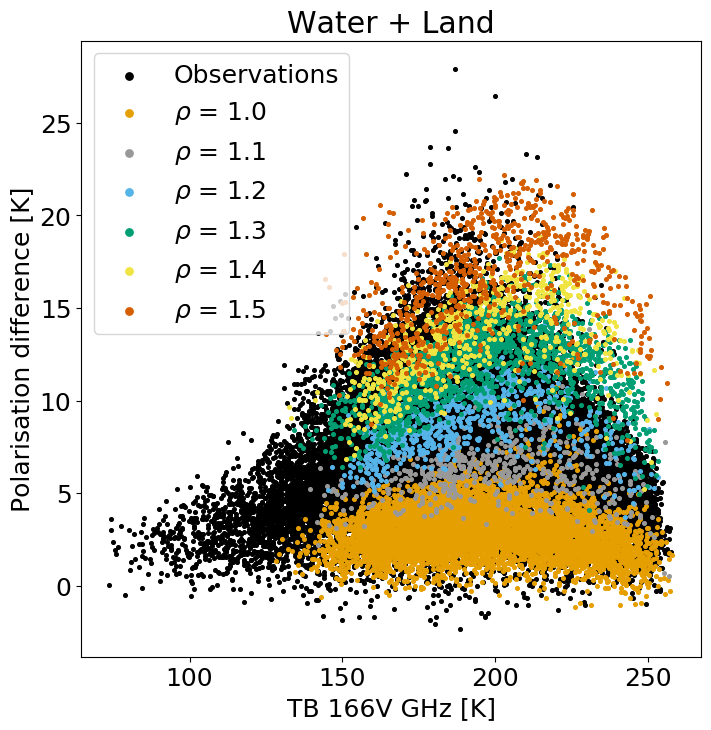
\includegraphics[width=4cm]{Figures/PD_water_varying_rho_water_land_esa.png}
	\caption{Same as Fig.~\ref{fig:PD_166} but for evans snow aggrergate. Water and land surface types are shown together.  }
	\label{fig:PD_esa}
\end{figure}

\begin{figure}[t]
	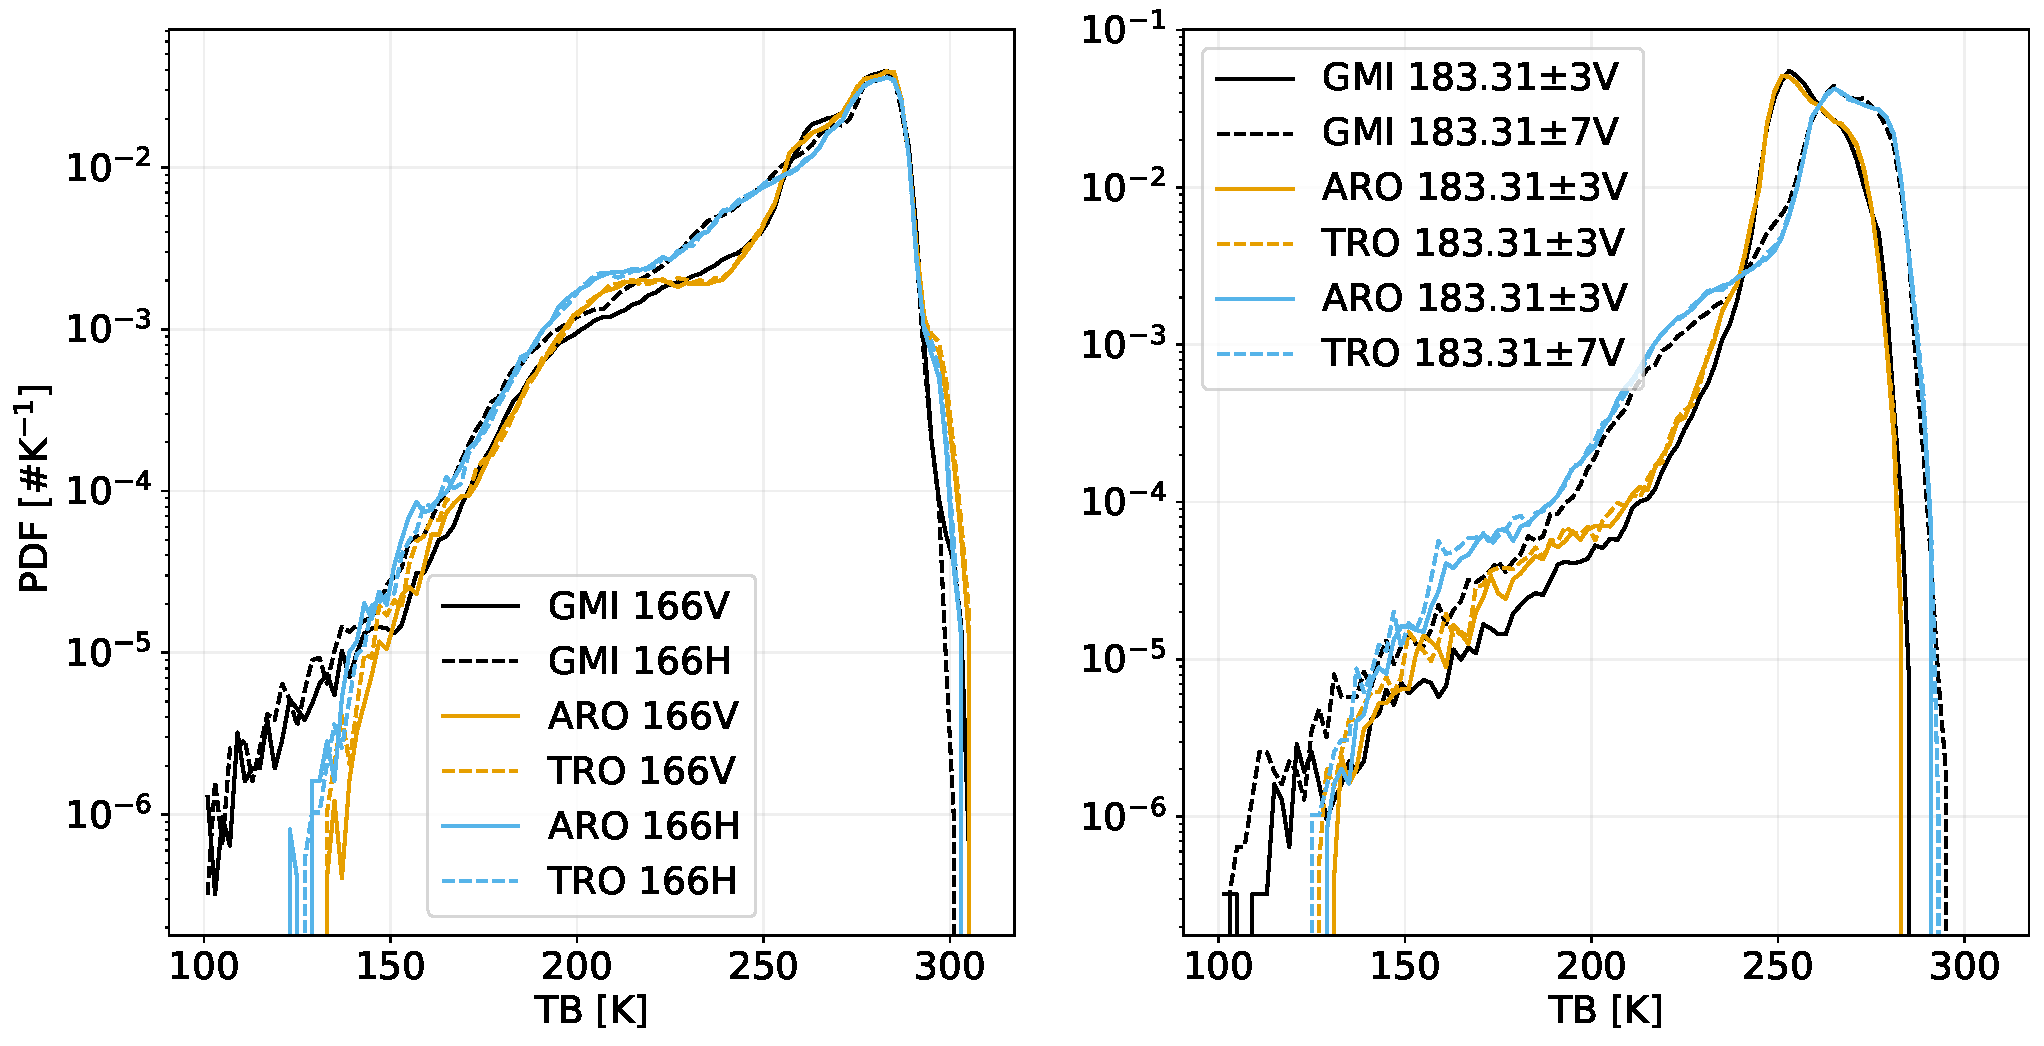
\includegraphics[width=6cm]{Figures/TB_esa.pdf}
	\caption{ Same as Fig.~\ref{fig:hist_TB} but for evans snow aggregate. }
	\label{fig:TB_esa}
\end{figure}

Figure~\ref{fig:PD_esa} shows the simulated PDs as a function of TB at 166V\,GHz for evans snow aggregate overlaid on the observed PDs. It is similar to Fig.~\ref{fig:PD_166}, except both water and land surface types are grouped together. Compared to Fig.~\ref{fig:PD_166}, quite similar behaviour of varying $\rho$ can be observed. However, $\rho = 1.4$ falls slightly short of simulating the PDs around 17\,K. Additionally, PDs to the left of 150\,K are also missed by the simulations. Both these effects are likely due to limitation of particle model. Implementing $\rho = 1.5$ can replicate a part of the highest observed PDs but it also gives larger frequency of falsely high PDs for TBs > 200\,K. 
%A comparison of divergences (not shown) between simulations and observations for a $\rho\in U[1, 1.4]$ and $\rho\in \mathcal{N}[1.2, 0.12]$ was also made, and again the uniformly distributed $\rho$ emerged as best performing.

Further, the TB distributions for the four channels of GMI is displayed in Fig.~\ref{fig:TB_esa}. For all four frequencies, evans snow aggregate fails in simulating the coldest TBs, but interestingly, the mismatch between simulations and observations in the intermediate zone is smaller than the one observed with large plate aggregate. This is am important result, which reinforces the fact constraining the microphysical assumptions to single habit and PSD, it not enough. In future, better agreements with observations can be achieved by more advanced microphysical schemes.  


\section{QRNN configuration and inputs}
%
\label{app:qrnn_conf}
In order to implement an optimal QRNN for the current application, several factors are crucial. The QRNN architecture that was considered for this application is described as follows:

\begin{enumerate}	
	
	\item QRNN predicts the posterior distribution in terms of quantiles. The quantiles are user defined, high resolution quantile fractions are allowed. For this study, 51 equally spaced quantile fractions between 1\% and 99\% were selected. 	
	
	\item The multiple hyper-parameters such as number of hidden layers, layer widths, batch size were selected by comparing the performance of the network over fixed set of values. Through this iterative approach, the network architecture with lowest mean quantile loss was chosen for all QRNN trainings presented in this study. Finally, a neural network with five hidden layers and 256 neurons in each layer was selected. The batch size was fixed at 256. 
	
	\item The update on the network parameters was made with SGD optimizer along with cosine annealing as the learning rate scheduler. We started with an initial learning rate of 1e-2 and trained for 50 epochs, and then the learning rate was reduced to 1e-3 and trained further for 50 epochs. Finally, the learning rate was reduced to 1e-4 and the model was trained for 100 epochs.
	Using a modified learning scheduler like this gave better calibration as compared to using only one kind of adaptive learning rate.
	
\end{enumerate}

While it is important to set-up an optimal neural network architecture, it is also crucial to find the best combination of input variables. Efficient retrieval performance requires the best combination of the training architecture and input data. The details about the training data are as follows: 

\begin{enumerate}
	
	\item The input vector space consists of TBs from the four high frequency channels of GMI ie., 166V\,\,GHz, 166H\,\,GHz, 183$\pm$3\,\,GHz, 183$\pm$7\,\,GHz. We also included 2\,\,m temperature, water vapour path, surface elevation and surface type as additional inputs to identify the environmental conditions. Seven surface types are considered : water, land, snow, seaice, coastlines, snow/land boundary and seaice/water boundary. We bundled snow/water boundary under snow, as GMI did not classify it separately. 
	
	\item The IWP has a very high dynamic range. A large majority of cases have very small or zero IWPs, but values as large at 25\,\,kg m$^{-2}$ also exist. Thus to facilitate the optimal use of data in the neural network, a loglinear transformation was applied. That is, all IWPs greater than 1.0\,\,kg m$^{-2}$  were transformed to natural logarithmic space, while the other IWPs remained unchanged. Additionally, all cases with IWP less 10$^{-4}$ were replaced by a small random number from the interval (10$^{-6}$, 10$^{-4}$).	
	
	\item To avoid over-fitting a ML training model, data augmentation is often used to increase the variability in the data by adding noise. For our model, random noise was added to TB in each training cycle or epoch. The noise was added according to the NE$\Delta$T. 
	
	\item A small randomisation of the surface types was also included to take include misclassification in the database. Comparisons of the simulations and observations showed that GPROF surface classification could be wrong, particularly in regions with mixed surface types. Thus to enhance the robustness of the machine learning model to these perturbations, the surface type of 1\% of the data was randomly shuffled at each epoch. 	
	
\end{enumerate}


\noappendix       %% use this to mark the end of the appendix section. Otherwise the figures might be numbered incorrectly (e.g. 10 instead of 1).

%% Regarding figures and tables in appendices, the following two options are possible depending on your general handling of figures and tables in the manuscript environment:

%% Option 1: If you sorted all figures and tables into the sections of the text, please also sort the appendix figures and appendix tables into the respective appendix sections.
%% They will be correctly named automatically.

%% Option 2: If you put all figures after the reference list, please insert appendix tables and figures after the normal tables and figures.
%% To rename them correctly to A1, A2, etc., please add the following commands in front of them:

\appendixfigures  %% needs to be added in front of appendix figures

\appendixtables   %% needs to be added in front of appendix tables

%% Please add \clearpage between each table and/or figure. Further guidelines on figures and tables can be found below.



\authorcontribution{TEXT} %% this section is mandatory

\competinginterests{TEXT} %% this section is mandatory even if you declare that no competing interests are present

\disclaimer{TEXT} %% optional section

\begin{acknowledgements}
TEXT
\end{acknowledgements}




%% REFERENCES

\bibliographystyle{copernicus}
\bibliography{references.bib}


%% Since the Copernicus LaTeX package includes the BibTeX style file copernicus.bst,
%% authors experienced with BibTeX only have to include the following two lines:
%%
%% \bibliographystyle{copernicus}
%% \bibliography{example.bib}
%%
%% URLs and DOIs can be entered in your BibTeX file as:
%%
%% URL = {http://www.xyz.org/~jones/idx_g.htm}
%% DOI = {10.5194/xyz}


%% LITERATURE CITATIONS
%%
%% command                        & example result
%% \citet{jones90}|               & Jones et al. (1990)
%% \citep{jones90}|               & (Jones et al., 1990)
%% \citep{jones90,jones93}|       & (Jones et al., 1990, 1993)
%% \citep[p.~32]{jones90}|        & (Jones et al., 1990, p.~32)
%% \citep[e.g.,][]{jones90}|      & (e.g., Jones et al., 1990)
%% \citep[e.g.,][p.~32]{jones90}| & (e.g., Jones et al., 1990, p.~32)
%% \citeauthor{jones90}|          & Jones et al.
%% \citeyear{jones90}|            & 1990



%% FIGURES

%% When figures and tables are placed at the end of the MS (article in one-column style), please add \clearpage
%% between bibliography and first table and/or figure as well as between each table and/or figure.

% The figure files should be labelled correctly with Arabic numerals (e.g. fig01.jpg, fig02.png).


%% ONE-COLUMN FIGURES

%%f
%\begin{figure}[t]
%\includegraphics[width=8.3cm]{FILE NAME}
%\caption{TEXT}
%\end{figure}
%
%%% TWO-COLUMN FIGURES
%
%%f
%\begin{figure*}[t]
%\includegraphics[width=12cm]{FILE NAME}
%\caption{TEXT}
%\end{figure*}
%
%
%%% TABLES
%%%
%%% The different columns must be seperated with a & command and should
%%% end with \\ to identify the column brake.
%
%%% ONE-COLUMN TABLE
%
%%t
%\begin{table}[t]
%\caption{TEXT}
%\begin{tabular}{column = lcr}
%\tophline
%
%\middlehline
%
%\bottomhline
%\end{tabular}
%\belowtable{} % Table Footnotes
%\end{table}
%
%%% TWO-COLUMN TABLE
%
%%t
%\begin{table*}[t]
%\caption{TEXT}
%\begin{tabular}{column = lcr}
%\tophline
%
%\middlehline
%
%\bottomhline
%\end{tabular}
%\belowtable{} % Table Footnotes
%\end{table*}
%
%%% LANDSCAPE TABLE
%
%%t
%\begin{sidewaystable*}[t]
%\caption{TEXT}
%\begin{tabular}{column = lcr}
%\tophline
%
%\middlehline
%
%\bottomhline
%\end{tabular}
%\belowtable{} % Table Footnotes
%\end{sidewaystable*}
%
%
%%% MATHEMATICAL EXPRESSIONS
%
%%% All papers typeset by Copernicus Publications follow the math typesetting regulations
%%% given by the IUPAC Green Book (IUPAC: Quantities, Units and Symbols in Physical Chemistry,
%%% 2nd Edn., Blackwell Science, available at: http://old.iupac.org/publications/books/gbook/green_book_2ed.pdf, 1993).
%%%
%%% Physical quantities/variables are typeset in italic font (t for time, T for Temperature)
%%% Indices which are not defined are typeset in italic font (x, y, z, a, b, c)
%%% Items/objects which are defined are typeset in roman font (Car A, Car B)
%%% Descriptions/specifications which are defined by itself are typeset in roman font (abs, rel, ref, tot, net, ice)
%%% Abbreviations from 2 letters are typeset in roman font (RH, LAI)
%%% Vectors are identified in bold italic font using \vec{x}
%%% Matrices are identified in bold roman font
%%% Multiplication signs are typeset using the LaTeX commands \times (for vector products, grids, and exponential notations) or \cdot
%%% The character * should not be applied as mutliplication sign
%
%
%%% EQUATIONS
%
%%% Single-row equation
%
%\begin{equation}
%
%\end{equation}
%
%%% Multiline equation
%
%\begin{align}
%& 3 + 5 = 8\\
%& 3 + 5 = 8\\
%& 3 + 5 = 8
%\end{align}
%
%
%%% MATRICES
%
%\begin{matrix}
%x & y & z\\
%x & y & z\\
%x & y & z\\
%\end{matrix}
%
%
%%% ALGORITHM
%
%\begin{algorithm}
%\caption{...}
%\label{a1}
%\begin{algorithmic}
%...
%\end{algorithmic}
%\end{algorithm}
%
%
%%% CHEMICAL FORMULAS AND REACTIONS
%
%%% For formulas embedded in the text, please use \chem{}
%
%%% The reaction environment creates labels including the letter R, i.e. (R1), (R2), etc.
%
%\begin{reaction}
%%% \rightarrow should be used for normal (one-way) chemical reactions
%%% \rightleftharpoons should be used for equilibria
%%% \leftrightarrow should be used for resonance structures
%\end{reaction}
%
%
%%% PHYSICAL UNITS
%%%
%%% Please use \unit{} and apply the exponential notation


\end{document}
